%%%%%%%%%%%%%%%%%%%%%%%%%%%%%%%%%%%%%%%%%%%%%%%%%%%%%%%%%%%%%%%%%%%%%%%%%%%%%%%%
% University of Western Ontario Thesis Template
% By: Justin Quinn Veenstra, 2010
% With thanks to Mr. (soon to be Dr.) Will Robertson.


\documentclass[12pt,twoside]{report}
%% Decomment next line to use PostScript fonts
%%\UsePackage{times}
%%%%%%%%%%%%%%%%%%%%%%%%%%%%%%%%%%%%%%%%%%%%%%%%%%%%%%%%%%%%%%%%%%%%%%%%
%%                                                                    %%
%%                    ***   I M P O R T A N T   ***                   %%
%%                                                                    %%
%% Fill in the following fields with the required information:        %%
%%  - \department{...}  name of the graduate department               %%
%%  - \degree{...}      name of the degree obtained                   %%
%%  - \author{...}      name of the author                            %%
%%  - \title{...}       title of the thesis                           %%
%%  - \gyear{...}       year of graduation                            %%
%%  - \super{...}    supervisor
%%  - \firstname, \middlename, \lastname... there is additional documentation by the actual fields, so I'll leave it at that
%%%%%%%%%%%%%%%%%%%%%%%%%%%%%%%%%%%%%%%%%%%%%%%%%%%%%%%%%%%%%%%%%%%%%%%%
\usepackage{appendix}
\usepackage{graphicx}
\usepackage{amsmath}
\usepackage[byname]{smartref}
%\usepackage{hyperref} %comment out for hardcopy
\usepackage{txfonts}
\usepackage{tocloft}


%My packages:
\usepackage{afterpage}
\usepackage{amssymb}
\usepackage{stmaryrd}
\usepackage{setspace}
\usepackage{attrib}
\usepackage{todonotes}
\usepackage{pgfplots}
\usepackage{subcaption}
%\usepackage{amsthm}
\usepackage{mdwlist}
\usepackage{listings}
\usepackage{tikz}
\usetikzlibrary{matrix,decorations.pathreplacing}


\newtheorem{thm}{Theorem}[section]


%\newcommand{\fjoin}{\,\bar{\varobar}\,}
\newcommand{\fjoin}{\varobar}

\newcommand{\hset}[1]{ \left\{ \! \left| \; #1 \; \right| \! \right\} }

\newcommand{\hjoin}[1][]{\varobar^{#1}}

\newcommand{\restrict}[2]{\left.#1\right|_{#2}}

\newcommand{\outerproduct}{\boxtimes}

\newcommand{\oiClCl}[1]{{ 	[\![ #1 ]\!] }}
\newcommand{\oiClOp}[1]{{ 	[\![ #1 )\!) }}
\newcommand{\oiOpCl}[1]{{ 	(\!( #1 ]\!] }}
\newcommand{\oiOpOp}[1]{{	(\!( #1 )\!) }}

\newcommand{\op}{\star}

\newcommand{\supp}{\text{supp}}

\newcommand{\R}[1][]{\mathcal{R}_{#1}}
\newcommand{\C}[1][]{\mathcal{C}_{#1}}

\newcommand*\diff{\mathop{}\!\mathrm{d}}

\lstset{language=Pascal}
\lstset{morekeywords={try, catch, finally, fi, proc, local}}

\def\ind[#1]{1_{#1}}
\def\extendedreal{\bar{\mathbb{R}}}
\def\hsetover[#1]{\mathbb{Z}^{#1}}

\makeatletter
\numberwithin{figure}{chapter}
\newenvironment{acknowledgements}%
{\clearemptydoublepage
 \begin{center}
  \section*{Acknowledgements}
 \end{center}
 \begingroup
}{\newpage\endgroup}

\newenvironment{dedication}%
{\clearemptydoublepage 
 \begin{center}
  \section*{Dedication}
 \end{center}
 \begingroup
}{\newpage\endgroup}

\newenvironment{preliminary}%
{\pagestyle{plain}\pagenumbering{roman}}%
{\pagenumbering{arabic}}

\addtoreflist{chapter}
\newtheorem{theorem}{Theorem}[section]
\newtheorem{lemma}[theorem]{Lemma}
\newtheorem{proposition}[theorem]{Proposition}
\newtheorem{corollary}[theorem]{Corollary}

\newenvironment{proof}[1][Proof]{\begin{trivlist}
\item[\hskip \labelsep {\bfseries #1}]}{\end{trivlist}}
\newenvironment{definition}[1][Definition]{\begin{trivlist}
\item[\hskip \labelsep {\bfseries #1}]}{\end{trivlist}}
\newenvironment{example}[1][Example]{\begin{trivlist}
\item[\hskip \labelsep {\bfseries #1}]}{\end{trivlist}}
\newenvironment{remark}[1][Remark]{\begin{trivlist}
\item[\hskip \labelsep {\bfseries #1}]}{\end{trivlist}}

\newcommand{\qed}{\nobreak \ifvmode \relax \else
      \ifdim\lastskip<1.5em \hskip-\lastskip
      \hskip1.5em plus0em minus0.5em \fi \nobreak
      \vrule height0.75em width0.5em depth0.25em\fi}

% Default values for title page.

%% To produce output with the desired line spacing, the argument of
%% \spacing should be multiplied by 5/6 = 0.8333, so that 1 1/2 spaced
%% corresponds to \spacing{1.5} and double spaced is \spacing{1.66}.
\def\normalspacing{1.25} % default line spacing


%% Define the "thesis" page style.
\if@twoside % If two-sided printing.
\def\ps@thesis{\let\@mkboth\markboth
   \def\@oddfoot{}
   \let\@evenfoot\@oddfoot
   \def\@oddhead{
      {\sc\rightmark} \hfil \rm\thepage
      }
   \def\@evenhead{
      \rm\thepage \hfil {\sc\leftmark}
      }
   \def\chaptermark##1{\markboth{\ifnum \c@secnumdepth >\m@ne
      Chapter\ \thechapter. \ \fi ##1}{}}
   \def\sectionmark##1{\markright{\ifnum \c@secnumdepth >\z@
      \thesection. \ \fi ##1}}}
\else % If one-sided printing.
\def\ps@thesis{\let\@mkboth\markboth
   \def\@oddfoot{}
   \def\@oddhead{
      {\sc\rightmark} \hfil \rm\thepage
      }
   \def\chaptermark##1{\markright{\ifnum \c@secnumdepth >\m@ne
      Chapter\ \thechapter. \ \fi ##1}}}
\fi

\pagestyle{thesis}
% Set up page layout.
\setlength{\textheight}{9in} % Height of the main body of the text
\setlength{\topmargin}{-.5in} % .5" margin on top of page
\setlength{\headsep}{.5in}  % space between header and top of body
\addtolength{\headsep}{-\headheight} % See The LaTeX Companion, p 85
\setlength{\footskip}{.5in}  % space between footer and bottom of body
\setlength{\textwidth}{6.25in} % width of the body of the text
\setlength{\oddsidemargin}{.25in} % 1.25" margin on the left for odd pages
\setlength{\evensidemargin}{0in} % 1.25"  margin on the right for even pages

% Marginal notes
\setlength{\marginparwidth}{.75in} % width of marginal notes
\setlength{\marginparsep}{.125in} % space between marginal notes and text

% Make each page fill up the entire page. comment this out if you
% prefer. 
\flushbottom

\setcounter{tocdepth}{3} % Number the subsubsections 
\def\normalspacing{1.25} % default line spacing

\newcommand\isco[1]{%
  \edef\@tempa{#1}%
  \def\@tempb{}%
  \ifx\@tempa\@tempb
	\else \\\underline{Co-Supervisor:}\vspace{0.35in}\\\dots\dots\dots\dots\dots\dots\dots\\{#1}\\
  \fi
}

\newcommand\isjoint[1]{%
  \edef\@tempa{#1}%
  \def\@tempb{}%
  \ifx\@tempa\@tempb
	\else \\\underline{Joint Supervisor:}\vspace{0.35in}\\\dots\dots\dots\dots\dots\dots\dots\\{#1}\\
  \fi
}

\newcommand\isalt[1]{%
  \edef\@tempa{#1}%
  \def\@tempb{}%
  \ifx\@tempa\@tempb
	\else \\\underline{Alternate Supervisor:}\vspace{0.35in}\\\dots\dots\dots\dots\dots\dots\dots\\{#1}\\
  \fi
}

\newcommand\isdefinedsig[1]{%
  \edef\@tempa{#1}%
  \def\@tempb{}%
  \ifx\@tempa\@tempb
	\else \\ \dots\dots\dots\dots\dots\dots\dots\\{#1}\\
  \fi
}
\newcommand\isdefinedspinetitle[1]{%
  \edef\@tempa{#1}%
  \def\@tempb{}%
  \ifx\@tempa\@tempb
	\else (Spine title: #1)\\
  \fi
}
\newcommand\coauthor[1]{%
  \edef\@tempa{#1}%
  \def\@tempb{}%
  \ifx\@tempa\@tempb
	\else \newpage \Large Co-Authorship Statement\normalsize\\\indent\\#1\\
  \fi
}

\newcommand\acknowlege[1]{%
  \edef\@tempa{#1}%
  \def\@tempb{}%
  \ifx\@tempa\@tempb
	\else \newpage \Large Acknowlegements\normalsize\\\indent\\#1\newpage
  \fi
}

%\renewcommand{\appendixtocname}{\Huge \textbf{List of Appendices} \normalsize}
\newcommand{\blank}{\hspace{-2mm}}
\newcommand{\super}{Dr. S. M. Watt} %supervisor
\newcommand{\superj}{} %joint supervisor, if there is one, leave blank if not (lbin)... only one of the three.
\newcommand{\superc}{} %co-supervisor, if there is one, leave blank if not (lbin)
\newcommand{\supera}{} %alternate supervisor, if there is one, leave blank if not (lbin)
\newcommand{\sco}{}  %member of supervisory committee
\newcommand{\sct}{}  %other member of supervisory committee (lbin)
\newcommand{\examo}{}  %examining committee (up to four, if less leave blank)
\newcommand{\examt}{}
\newcommand{\examth}{}
\newcommand{\examf}{}
\newcommand{\department}{Computer Science}
\newcommand{\degree}{Masters of Science}
\newcommand{\firstname}{Mike}
\newcommand{\middlename}{}
\newcommand{\lastname}{Ghesquiere}
%\renewcommand{\author}[1]{\ifx\empty#1\else\gdef\@author{#1}\fi} 
\newcommand{\authorname}{{\firstname} {\middlename} {\lastname}}
\newcommand{\titl}{Domain Decomposition, Integration, and Inclusion-Exclusion}
\newcommand{\spinetitle}{}%only if the above is more than 60 characters
\newcommand{\thesisformat}{Monograph} %or Integrated Article
\newcommand{\gyear}{\number\year}
\newcommand{\makecoauthor}{
%Type information about coauthorship here/
}
\newcommand{\makeacknowlege} {
%Type in acknowlegements here
}
\newcommand{\listappendixname}{List of Appendices}
\newlistof{myappendices}{app}{\listappendixname}
\newcommand{\myappendices}[1]{%
\addcontentsline{app}{myappendices}{#1}\par}

\renewcommand{\maketitle}
{\begin{titlepage}
   \setcounter{page}{1}
   %% Set the line spacing to 1 for the title page.
   %\begin{spacing}{1} 
   \begin{large}
   \begin{center}
      \mbox{}
      \vfill
      {\MakeUppercase{\titl}}\\
      \isdefinedspinetitle{\spinetitle}
      (Thesis format: \thesisformat)\\
      \vfill
      by \\
      \vfill
      {\firstname} \underline{\lastname}\\
      \vfill
      Graduate Program in {\department}\\
      \vfill
		A thesis submitted in partial fulfillment\\
		of the requirements for the degree of\\
		\degree\\
		\vfill
		The School of Graduate and Postdoctoral Studies\\
		The University of Western Ontario\\
		London, Ontario, Canada\\
		\vfill
      {\copyright} {\authorname} {\gyear}  \\
      \vspace*{.2in}
   \end{center}
   \end{large}
%   \end{spacing}
   \end{titlepage}

}%\maketitle

\newcommand{\makecert}{
   \setcounter{page}{2}
\vfill
\begin{center}
\large
THE UNIVERSITY OF WESTERN ONTARIO\\
School of Graduate and Postdoctoral Studies\\
\vfill
\textbf{CERTIFICATE OF EXAMINATION}
\end{center}

\vfill
\begin{table}[ht]
\begin{minipage}[t]{0.5\linewidth} %tabular instead?
\begin{tabular}{l}
\underline{Supervisor:}\vspace{0.35in}
\isdefinedsig{\super}
\isco{\superc}
\isjoint{\superj}
\isalt{\supera}
\\
\underline{Supervisory Committee:}\vspace{0.35in}
\isdefinedsig{\sco}\vspace{0.15in}
\isdefinedsig{\sct}
\end{tabular}
\vfill
\end{minipage}
\hspace{0.5in}
\begin{minipage}[t]{0.5\linewidth}
\begin{tabular}{l}
\underline{Examiners:} \\\vspace{.5cm}
\isdefinedsig{\examo}\\
\isdefinedsig{\examt}\\
\isdefinedsig{\examth}\\
\isdefinedsig{\examf}
\end{tabular}
\vfill
\end{minipage}
\vfill
\end{table}
\vfill
\begin{center}
The thesis by \\ \vfill
\textbf{\firstname{} \middlename{} \underline{\lastname}}\\
\vfill
entitled:\\\vfill
\textbf{\titl}\\\vfill
is accepted in partial fulfillment of the \\
requirements for the degree of\\
\degree\\
\end{center}
\begin{table}[ht]
\begin{minipage}[t]{0.5\linewidth}
\begin{tabular}{l}
\dots\dots\dots\dots\dots\\
Date
\end{tabular}
\end{minipage}
\hspace{0.5in}
\begin{minipage}[t]{0.5\linewidth}
\begin{tabular}{l}
\dots\dots\dots\dots\dots\dots\dots\dots\dots\dots\\
Chair of the Thesis Examination Board
\end{tabular}
\end{minipage}
\end{table}

}

\makeatother
\begin{document}

%% ***   NOTE   ***
%% You should put all of your '\newcommand', '\newenvironment', and
%% '\newtheorem's (in other words, all the global definitions that you
%% will need throughout your thesis) in a separate file and use
%% "\input{filename}" to input it here.


%% This sets the page style and numbering for preliminary sections.
\begin{preliminary}

%% This generates the title page from the information given above.
\maketitle
\addcontentsline{toc}{chapter}{Certificate of Examination}
\makecert
\newpage
%\addcontentsline{toc}{chapter}{Co-Authorship Statement}
%\coauthor{\makecoauthor}  %comment this out if none
%\newpage
\addcontentsline{toc}{chapter}{Acknowlegements}
%\acknowlege{\makeacknowlege}	%as above
\addcontentsline{toc}{chapter}{Abstract}
\Large\begin{center}\textbf{Abstract}\end{center}\normalsize
%%  ***  Put your Abstract here.   ***
%% (150 words for M.Sc. and 350 words for Ph.D.)

Mathematic notation has been dominated by sets and, when repeated elements are required, sequences generally make an appearance.
Historical inertia has caused these structures to be used in many situations where they are ill-suited often evidenced by phrases like "without loss of generality", "up to ordering of terms", "up to a sign".
However, by tackling these problems instead with more apt data structures, we can eliminate some of these stipulations and more formally reduce symmetric cases in reasoning.
In particular, this thesis will deal with \emph{hybrid sets} (that is, signed multisets), as well \emph{hybrid functions} (that is, functions with hybrid sets for their domain) with applications in piecewise functions, integration on manifolds, (...).
More than just an aesthetic change, by allowing negative multiplicity (even if it would not make physical sense), we may symblically manipulate structures in ways that might otherwise be cumbersome or inefficient.

% word count?!?!?

\vfill
\textbf{Keywords:} Hybrid set, Signed multiset, Integration on chains, Inclusion-Exclusion, (...)
\newpage
\tableofcontents\newpage
\newpage
\addcontentsline{toc}{chapter}{List of Figures} \listoffigures \newpage
%\addcontentsline{toc}{chapter}{List of Tables} \listoftables \newpage
%\addcontentsline{toc}{chapter}{List of Appendices}\listofmyappendices\newpage
%\addcontentsline{toc}{chapter}{List of Abbreviations, Symbols, and Nomenclature}\large List of Abbreviations, Symbols, and Nomenclature \normalsize \newpage
\end{preliminary}
%% End of the preliminary sections: reset page style and numbering.

%%%%%%%%%%%%%%%%%%%%%%%%%%%%%%%%%%%%%%%%%%%%%%%%%%%%%%%%%%%%%%%%%%%%%%%%
%%                                                                    %%
%%                    ***   I M P O R T A N T   ***                   %%
%%                                                                    %%
%% Put your Chapters here; the easiest way to do this is to keep each %%
%% chapter in a separate file and \include all the files right here.  %%
%% Note that each chapter file should start with the line             %%
%% "\chapter{ChapterName}".  Note that using "\include" instead of    %%
%% "\input" makes each chapter start on a new page.                   %%
%%%%%%%%%%%%%%%%%%%%%%%%%%%%%%%%%%%%%%%%%%%%%%%%%%%%%%%%%%%%%%%%%%%%%%%%

\chapter{Introduction}
\doublespacing


%%%%%%%%%%%%%%%%%%%%%%%%%%%%%%%%%%%%%%%%%
% MOTIVATION
%%%%%%%%%%%%%%%%%%%%%%%%%%%%%%%%%%%%%%%%%
\section{Motivation}


%(Unordered pairs \cite{EWD:EWD1223} ?)	
Some data structures in mathematics are more widely adopted than others and none more than Cantor's notion of sets.
The very foundations of mathematics lie in set theory: numbers are defined in terms of sets as are ordered tuples 
which in turn lead to relations, functions, sequences and from there branches into countless other structures.
But this trunk typically omits a satisfactory treatment of several \emph{generalized sets}.
For example, it is difficult to begin speaking about \emph{hybrid sets} without immediately punctuating, 
\emph{``---that is, multi-sets with negative multiplicity''}.


It is a statement of progress that multi-sets have even entered into common mathematical parlance.
On the other hand, sequences need no introduction and one can easily represent a multi-set by a sequence: 
if an element occurs in a multi-set with multiplicity $n$, ensure that it's in the corresponding sequence $n$ times as well.
In this way, sequences are often used \emph{in place of} multi-sets with the added structure of an ordering.
Indeed,  \emph{``why not?''}, even if the order of elements is not needed, \emph{``surely it can't hurt?''}


Consider the \emph{Fundamental Theorem of Arithmetic}:
\begin{quote}
	``Every positive integer, except 1, is a product of primes. 
	(\ldots) 
	The standard form of $n$ is unique; 
	apart from rearrangement of factors, $n$ can be expressed as a product of primes in one way only.''
	\attrib{Hardy and Wright 1979, p.2-3}
\end{quote}
By recognizing the possibility of rearranging factors, the authors implicitly define type the ``product of primes'' as a sequence rather than, more aptly a multi-set.
For iterated, commutative operators (e.g. $\sum, \prod, \bigcap, \bigcup$), the order of terms is irrelevant so then, 
\emph{``why order terms to begin with?''}
Reisig \cite{reisig1985petri} uses multi-sets to define relation nets where 
``\ldots several individuals of some sort do not have to be distinguished", and moreover
 ``One \emph{should not} be forced to distinguish individuals if one doesn't wish to.  This would lead to overspecification''
(emphasis added). The same applies here.


Secondly --- and this is a more subtle and subjective point --- 
the empty sequence is not nearly as enshrined as the empty set.
Whereas the empty set is often the first thing that comes to mind when searching for trivial cases or counter-examples,
the empty sequence is not usually so readily recalled.
Despite the empty sequence being just as well-defined as the empty set; it tends to be treated as an aberrant case.
In the case of iterated operators over an empty set, it is simply the respective identity.
In the case of $\prod$, this is 1, and so 1 \emph{is} a product of primes.
It is uniquely, the product of the empty set of primes.
Similarly, a sequence containing just one element is still a sequence but this also can be easy to forget.
Some definitions will also disregard this to say, ``is prime or the product of primes''. 
Whether this is extra specificity is a fault to the authors or simply a reminder to readers, the point remains the same.
The perception of sequences can be misleading in ways in which sets are not often misconstrued.
Stripped of these qualifications we are left with the more succinct:
\begin{quote}
	``Every positive integer is the product of a unique multiset of primes.''
\end{quote}


It goes deeper than a matter of aesthetics. 
Sets are certainly flexible objects and it is tempting to take a minimal approach to the tools required in one's toolbox.
But the algebra of sets, is a fairly restrictive one.
Consider the sets $[a,b) = \{ x \; |\; a \leq x < b \}$ and $[b,c) = \{ x \;|\: b \leq x < c \}$.
Their union $[a,b) \cup [b,c)$ will depend heavily on the relative ordering of $a$, $b$ and $c$. 
More often, as in integration what one really wants is $[a,b) + [b,c) = [a,c)$.
When boolean algebra and numeric algebra interface, results can get unnecessarily messy.
Hybrid sets will allow us to remove this tension, by committing fully to numeric algebra
In this spirit that we will graft hybrid sets into areas of mathematics where current approaches are unsatisfactory.





%%%%%%%%%%%%%%%%%%%%%%%%%%%%%%%%%%%%%%%%%
% OBJECTIVES
%%%%%%%%%%%%%%%%%%%%%%%%%%%%%%%%%%%%%%%%%		
\section{Objectives}


This thesis will include and extend the work of \cite{carette2010} on hybrid sets and their applications.
In particular we will take as inspiration the following identity for integrals:
\begin{equation}
	\int_a^b f(x) \diff x = -\int_b^a f(x) \diff x
\end{equation}
This allows for the identity
\begin{equation}
	\int_a^c f(x) \diff x = \int_a^b f(x) \diff x + \int_b^c f(x) \diff x
\end{equation}
regardless of the ordering of $a$, $b$ and $c$.
One can think of the region from $a$ to $c$ being partitioned into $a$ to $b$ and $b$ to $c$.
But this is not a partition in the usual sense.
Rather than the union of disjoint subsets, it is a sum of oriented subsets: a generalized partition.
This is a rather nice behaviour that would be nice to emulate in other contexts as well.


We will consider several different applications.
When matrices are represented in terms of block submatrices, 
the sum or product can vary depending on operand block sizes.
Representing the regions of a block matrix with hybrid sets will allow for all cases to be consolidated into one;
no matter how those blocks may overlap.
Lebesgue integration relies on measurable sets and also does not naturally support orientation.
Here, hybrid sets will allow us to evaluate integrals like $\int_1^0 1_{\mathbb{R} \setminus \mathbb{Q}} \diff x = -1$
Finally, we will consider the convolution of piecewise interval functions.
Typically different equations are used depending on the relative length of intervals but with hybrid sets we can condense this
into one general equation and ignore the interval lengths altogether.


Unifying all of this is the argument that hybrid sets are a very useful structure and there are many instances where existing
structures ought to be replaced.
Hopefully these examples will provide inspiration to the reader to recognize similar situations elsewhere as well.




%%%%%%%%%%%%%%%%%%%%%%%%%%%%%%%%%%%%%%%%%
% RELATED WORK
%%%%%%%%%%%%%%%%%%%%%%%%%%%%%%%%%%%%%%%%%
\section{Related Work}


It is difficult to date the origin of multisets.
Although the term itself was coined by De Bruijn in corresponces with Knuth \cite{knuth2014art},
the thought of a ``collection of objects that may or may not be distinguished'' is as old as tally marks. 
In regards to the generalization to \emph{signed} multisets, Hailperin \cite{hailperin1986boole} 
suggests that Boole's 1854 \emph{Laws of Thought} \cite{boole1854investigation} is actually a treatise of signed multisets.
Whether this was Boole's intent is debateable.
Sets with negative membership explicitly began to appear in \cite{whitney1933characteristic} and were 
formalized under the name Hybrid sets in Blizard's extensive work with generalized sets \cite{blizard1988, blizard1990} 
Although hybrid set and signed multiset are the most common nomenclature, other names appearing in literature include
multiset (specifying positive when speaking of unsigned multisets) \cite{reisig1985petri} 
and integral multiset \cite{wildberger2003new}. 


Existing explicit applications of hybrid sets are currently limited.
Loeb \emph{et al.} \cite{damiani1991, loeb1992} use hybrid sets to generalize several combinatoric identities to negative values.
Bailey \emph{et al.} \cite{bailey2009hypergraphic} and Ban\^{a}tre \emph{et al.} \cite{banatre2006} 
have also had success with hybrid sets in chemical programming. 
Representing a solution is represented as a collection of atoms and molecules, 
negative multiplicities are treated as ``antimatter'' . 
For a deeper overview and systemization of generalized sets, see \cite{singh2007, singh2008systematization}.
These these ideas allow symbolic computation on functions defined piecewise \cite{carette2010}.


%%%%%%%%%%%%%%%%%%%%%%%%%%%%%%%%%%%%%%%%%
% MOTIVATION
%%%%%%%%%%%%%%%%%%%%%%%%%%%%%%%%%%%%%%%%%
\section{Thesis Outline}


In chapter 2, the foundations for hybrid sets and functions with hybrid set domains will be laid. 
This will provide us with formal definitions and some immediate applications to piecewise functions will be presented.
Chapter 3 will see hybrid domains applied towards symbolic matrix algebra.
Addition has already been considered \cite{carette2010}, but this will be extended to multiplication as well.
In chapter 4, hybrid functions will be applied towards integration. 
We will start from foundations and use hybrid functions to allow for an oriented Lebesgue integral.
We will then show how hybrid sets naturally come up in Stokes' theorem with the boundary operator.
Finally in chapter 5, hybrid sets will be applied towards convolution of piecewise functions.



















\chapter{Hybrid Set Theory}


%%%%%%%%%%%%%%%%%%%%%%%%%%%%%%%%%%%%%%%%%
%
% PIECEWISE
%
%%%%%%%%%%%%%%%%%%%%%%%%%%%%%%%%%%%%%%%%%


The motivation behind hybrid sets and functions can be traced to wanting a better approach to piecewise functions
and closely related to that is a more generalized notion of a partition.
In general, we assume a piecewise function $f : P \to X$ will take the form:
\begin{equation}
	\label{eq_fP}
	f(x) = 
	     \begin{cases}
	       f_1(x) & x \in P_1 \\
	       f_2(x) & x \in P_2 \\ 
	       \vdots & \vdots \\
	       f_n(x) & x \in P_n
	     \end{cases}
\end{equation}
where the set $\{ P _ i \}$ is a partition of $P$ the domain of $f$.
Each subfunction $f_i$, we can only safely assume is defined over its respective partition $f_i : P_i \to X$.
Frequently these partitions are not expressed explicitly as sets but rather as conditions.
For example, the absolute value function is far more commonly written out as
\begin{equation*}
	\abs(x) = \begin{cases} -x & x < 0 \\ x & x \geq 0 \end{cases}
	\;\;\;\;\;\;\;\;\;\text{rather than}\;\;\;\;\;\;\;\;\;
	\abs(x) = 
	\begin{cases}
		-x & \{x \;|\; x \in \mathbb{R} \wedge x < 0\}  \\ 
		x & \{x \;|\; x \in \mathbb{R} \wedge x \geq 0 \}
	\end{cases}
\end{equation*}
but using conditions rather than the sets they define can be seen as just a shorthand. 


One thing that should be noted is that sometimes there are extra conditions which are bundled in.
As pieces of a partition, the sets generated must be disjoint so we must ensure these conditions are mutually exclusive.
A common heuristic is to treat these conditions as a series of \emph{else-if} statements.
For example \emph{Maple}'s \texttt{piecewise} function:
\begin{quote}
	\texttt{piecewise(cond\_1, f\_1, cond\_2, f\_2, \ldots, cond\_n, f\_n, f\_otherwise)} 
\end{quote}	
will evaluate each \texttt{cond\_1} in order and when one evaluates to true, the corresponding \texttt{f\_i} is then evaluated.
Finally if all of \texttt{cond\_i} evaluate to false then \texttt{f\_otherwise} is used.
Hence the partitions corresponding to each \texttt{cond\_i} is \emph{not} just $\{ x \;|\; \texttt{cond\_i}(x) \}$
but instead the set where \texttt{cond\_i} is true and \emph{all preceding} conditions are also false.



Although the notation used in (\ref{eq_fP}) is fine for piecewise functions with only a few terms such as $\abs$,
it quickly becomes unwieldy when one wants to add more pieces.
So instead we will use the \emph{join} of disjoint function \emph{restrictions}.
\begin{definition}
	Given a function $f:X \to Y$ and any subset of the domain $Z \subset X$, 
	the \textbf{restriction of $\boldsymbol{f}$ to $\boldsymbol{Z}$} is the function $f|_Z : Z \to Y$, 
	such that $f|_Z(x) = f(x)$ for all $x \in Z$.
\end{definition}


There are several ways which one could define a join operator; specifically how one deals with intersections.
One could favor the first function as Maple does, but we will take the stance that the intersection is poorly defined.
\begin{definition}
	Define $\fjoin$, the \textbf{join} of two functions, $f$ and $g$ by:
	\begin{equation}
	\label{def:fjoin}
		f \fjoin g =  
		\left\{
	     		\begin{array}{lr}
	       		f(x) & \text{if } g(x) = \bot \\
	       		g(x) & \text{if } f(x) = \bot \\
	       		\bot & otherwise
	     		\end{array}
	   	\right.
	\end{equation}
\end{definition}
As such if $f:X \to Y$ and $g:S \to T$ then the join will be defined not on the union of $X$ and $S$ but on their 
\emph{symmetric difference}.
Together these definitions allow us to re-write the piecewise function in (\ref{eq_fP}) as:
\begin{equation*}
	f = \restrict{f}{P_1} \fjoin \restrict{f}{P_2} \fjoin \ldots \fjoin \restrict{f}{P_n}
\end{equation*}


Now consider arithmetic of two piecewise functions. Let $f$ and $g$ be two piecewise functions
$f = \left(\restrict{f_1}{P_1} \fjoin \restrict{f_2}{P_2} \fjoin \restrict{f_3}{P_3} \right)$ 
and $g= \left( \restrict{g_1}{Q_1} \fjoin \restrict{g_2}{Q_2} \right)$.
To compute the sum $f+g$ we need to consider each possible intersection of partitions of $P$ and partitions of $Q$.
In this case, the result is generally a piecewise function with 6 terms:
\begin{align*}
	(f+g) = \;
	&\restrict{(f_1+g_1)}{P_1 \cap Q_1} 
		\;\fjoin\; \restrict{(f_1+g_2)}{P_1 \cap Q_2} 
		\;\fjoin\; \restrict{(f_1+g_3)}{P_1 \cap Q_3}\notag\\
	&\restrict{(f_2+g_1)}{P_2 \cap Q_1} 
	 	\;\fjoin\; \restrict{(f_2+g_2)}{P_2 \cap Q_2} 
	 	\;\fjoin\; \restrict{(f_2+g_3)}{P_2 \cap Q_3}
\end{align*}
In specific cases, some terms may be eliminated as intersection would is impossible.
In general, assuming no degenerate intersections, 
the sum of an ``$n$-piece'' function and ``$m$-piece'' function will give a piecewise function with $n\times m$ pieces.


Another perspective to take is to first find a \emph{common refinement} of ${P=\{P_i\}_{i\in I}}$ 
and ${Q=\{Q_j\}_{j\in J}}$. In the above example we selected the refinement:
\begin{equation*}
	R=\Big\{\;
		(P_1 \cap Q_1),\;(P_2 \cap Q_1),\;(P_3 \cap Q_1),\;
		(P_1 \cap Q_2),\;(P_2 \cap Q_2),\;(P_3 \cap Q_2) \;
	\Big\}
\end{equation*}
That is, for each $P_i$ in the partition $P$, there is a subset of $R$ which will partition $P_i$ 
(namely $P_i = \{ (P_i \cap Q_1), (P_i \cap Q_2) \}$ and so $R$ is a \emph{refinement} of $P$.
Similarly $R$ also a refinement of $Q$ and so we say it is a \emph{common refinement} of $P$ and $Q$.


Finding common refinements gives a large increase in the number of terms required, 
in part, due to a restrictive view of partitions.
Conceptually, what one wishes out of a partition is a family of subsets which will ``sum'' up to the original.
With boolean sets, some additional constraints are imposed as we don't have a very good notion of subtraction.
However, by using non-boolean sets we allow for negative sets to cancel any double-counting
as such disjointness no longer needs to be enforced.
Over this chapter we will consider such generalized partitions and the structures to support them.
We will also see how this allows for us to eliminate the multiplicative increase in terms when flattening the sum
(or product) of two piecewise functions.





%%%%%%%%%%%%%%%%%%%%%%%%%%%%%%%%%%%%%%%%%
%
% HYBRID SET
%
%%%%%%%%%%%%%%%%%%%%%%%%%%%%%%%%%%%%%%%%%
\section{Hybrid Sets}


We shall consider \emph{hybrid sets}.
One can view traditional boolean sets as an indicator function 
which maps each member element to 1 and each non-member to 0.
A \emph{multiset} (or \emph{bag}) extends this by allowing multiple copies of the same element.
The indicator function of a multiset would therefore range over $\mathbb{N}_0$, the set of non-negative integers.
Hybrid sets take this one step further allowing for an element to occur \emph{negatively many} times.


\begin{definition}
	Let $U$ be a universe, then any function $U \to \mathbb{Z}$ is called a \textbf{hybrid set}.
	We denote the collection of all hybrid sets over a universe by $\hsetover[U]$.
\end{definition}


By universe, we just mean a (traditional) set that \emph{contains everything we may be interested in}.
This is admittedly ague but we will rarely be interested in everything in the universe or its exact size.
It is simply a compact way for us to talk about ``everything else''.
But we will need some notation to make functions resemble sets.


\begin{definition}
	Let $H$ be a hybrid set. 
	Then we say that $H(x)$ is the \textbf{multiplicity} of the element $x$. 
	We write, $x \in^n H$ if $H(x)=n$. 
	Furthermore we will use $x \in H$ to denote $H(x)\neq 0$ (or equivalently, $x \in^n H$ for $n\neq 0$).
	Conversely, $x \notin H$ denotes $x \in^0 H$ or $H(x)=0$.
	The symbol $\emptyset$ will be used to denote the empty hybrid set for which all elements have multiplicity 0.
	Finally the \textbf{support of a hybrid set} is the (non-hybrid) set $\supp\;H$,
	where $x \in \supp\;H$ if and only if $x \in H$
\end{definition}


We will use the notation:
\begin{equation*}
	H = \hset{x_1^{m_1}, x_2^{m_2},\ldots}
\end{equation*}
to describe the hybrid set $H$ where the element $x_i$ has multiplicity $m_i$. 
We allow for repetitions in $\{ x_i \}$ but interpret the overall multiplicity of an element $x_i$ as 
the sum of multiplicities among copies. 
For example, $H=\hset{a^1, a^1, b^{-2}, a^3, b^1} = \hset{a^5, b^{-1}}$. 
The latter will generally be preferred as all $a$'s and $b$'s have been collected together as such
a writing in which $x_i \neq x_j$ for all $i \neq j$ is referred to as a \textbf{normalized form} of a hybrid set. 


Traditional sets use the operations $\cup$ union, $\cap$ intersection, and $\setminus$ complementation.
These correspond to the Boolean point-wise $\vee$ \texttt{OR}, $\wedge$ \texttt{AND}, and $\neg$ \texttt{NOT} 
operations. That is, for two sets $A$ and $B$, then $(A \cup B)(x) = A(x) \vee B(x)$.
One \emph{could} extend these for hybrid sets using point-wise min and max 
\cite{blizard1988, blizard1990, girish2012multiset, singh2011complementation}
but this is not very natural.
Rather, our primitive hybrid set operations should derive from our primitive point-wise operators.
When dealing with hybrid sets with multiplicities over the integers, we have the ring $(\mathbb{Z}, +, \times)$.
Thus we will define $\oplus$, $\ominus$, and $\otimes$ by point-wise $+$, $-$, and $\times$ respectively.


\begin{definition}
	For any two hybrid sets $A$ and $B$ over a common universe $U$, 
	we define the operations $\oplus, \ominus, \otimes : \mathbb{Z}^U \times \mathbb{Z}^U \to \mathbb{Z}^U$ 
	such that for all $x \in U$:
	\begin{align}
		(A \oplus B)(x) 	&= A(x) + B(x) \\
		(A \ominus B)(x) 	&= A(x) - B(x) \\
		(A \otimes B)(x) 	&= A(x) \cdot B(x)
	\end{align}
	We also define, $\ominus A$ as $\emptyset \ominus A$ and for $c \in \mathbb{Z}$:
	\begin{equation}
		(cA)(x) = c \cdot A(x)
	\end{equation}
\end{definition}


\begin{definition}
	We say $\boldsymbol{A}$ \textbf{and} $\boldsymbol{B}$ \textbf{are disjoint} if and only if $A \otimes B = \emptyset$
\end{definition}
For boolean sets $A$ and $B$, disjointness would be defined by $A \cap B = \emptyset$.
If we consider these boolean sets as simply hybrid sets with multiplicity 0 or 1 then the operations $\cap$ and $\otimes$
identically correspond to element-wise $\texttt{AND}$.


From these definitions, we can use hybrid sets to model various objects that would traditionally be described otherwise. 
For example, any positive rational number can be represented as a hybrid set over the primes.
\begin{equation*}
	(\mathbb{Z}^\mathbb{P}, \oplus) \simeq (\mathbb{Q}_+,\times)
\end{equation*}
For a positive rational number $a/b$, both $a$ and $b$ being integers will have a prime decomposition: 
$a=(p_1^{m_1}\cdot p_2^{m_2} \cdot \ldots)$ and $b=(q_1^{n_1} \cdot q_2^{n_2} \cdot \ldots)$
then there is the group isomorphism $f$ given by:
\begin{equation*}
	f(a/b) = \hset{p_1^{m_1}, p_2^{m_2}, \ldots} \ominus \hset{q_1^{n_1}, q_2^{n_2}, \ldots}
\end{equation*}
Furthermore, we have the equivalence $ca/cb = a/b$ for free by writing the hybrid set in normalized form
(e.g. $2/4 = \hset{2^1, 2^{-2}} = \hset{2^{-1}} = 1/2$).
One could also think of the roots and asymptotes of a rational polynomial as a hybrid set over the underlying ring:
\begin{equation*}
	\frac{(x-2)}{(x-1)^2(x+1)} \;=\; \hset{ 2^1, 1^{-2}, -1^{-1} }
\end{equation*}
Depending on the context, a negative multiplicity could take many different meanings.
Rather than attach a single rigid concept, we will keep this flexibly abstract sometimes.
In these examples we used the multiplicity as an exponent in other cases it is more aptly a coefficient  or as orientation.


All Boolean sets can be trivially converted to hybrid sets.
For a set $X$, this is done simply by taking $H(x)=1$ if $x \in X$ and $H(x)=0$ if $x \notin X$.
We will often perform this conversion silently by applying hybrid set operators to Boolean sets.
The reverse conversion: the reduction of a hybrid set to a boolean set is not always possible.


\begin{definition}
	Given a hybrid set $H$ over universe $U$, 
	if for all $x \in U$ $H(x)=1$ or $H(x)=0$ then we say that \textbf{$\boldsymbol{H(x)}$ is reducible}.
	If $H$ is reducible then we denote the \textbf{reduction of $\boldsymbol{H}$} by $\mathcal{R}(H)$ 
	as the (non-hybrid) set over $U$ with the same membership.  
\end{definition}


In Boolean set theory, a partition of $X$ is a collection of subsets of $X$ such that $X$ is a disjoint union of the subsets.
When dealing with hybrid sets we no longer have (or rather choose not to use) union but use point-wise sum instead.
For disjoint, reducible hybrid sets, point-wise sum and union agree but we will be even more accommodating 
and allow for \emph{any} family of sets which sum to a hybrid set to be a (generalized) partition.


\begin{definition}
	A \textbf{generalized partition $\boldsymbol{P}$ of a hybrid set $\boldsymbol{H(x)}$} is a family of hybrid sets
	${P=\{P_i \}_{i=1}^n}$ such that:
	\begin{equation}
		H = P_1 \oplus P_2 \oplus \ldots \oplus P_n
	\end{equation}
	We say that \textbf{$\boldsymbol{P}$ is a strict partition of $\boldsymbol{H}$} if 
	$P_i$ and $P_j$ are disjoint for all $i \neq j$.
\end{definition}


If a set $H$ is reducible, then strict generalized partitions will correspond with the traditional notion of a partition.
A traditional partition will be a disjoint cover of $H$ and for disjoint reducible sets, point-wise sum and union agree.
Hence $\bigcup_i P_i = \bigoplus_i P_i$. 
Conversely, if $H$ is reducible and the sum of disjoint hybrid sets, then $P_i$ must all be reducible as well.


This does not hold for a non-strict partition of a reducible hybrid set.
Consider the interval $[0,1]$ as a hybrid set (that is, $H(x)=1$ if $0 \leq x \leq 1$ and $H(x)=0$ otherwise).
Then $P = \big\{\; [0,2], \;\ominus (1,2] \; \big\}$ is a generalized partition of $H$. 
A generalized partition of a reducible set is strict if and only if each generalized partition is reducible.





%%%%%%%%%%%%%%%%%%%%%%%%%%%%%%%%%%%%%%%%%
% Hybrid Function
%%%%%%%%%%%%%%%%%%%%%%%%%%%%%%%%%%%%%%%%%
\section{Hybrid Functions}
\label{sec:HybridFunction}


A function is typically defined as a mapping from elements of one set to another set.
We will consider functions which have hybrid sets as their domain (but still map to traditional sets) 
which we will call \emph{hybrid functions}.
We will define hybrid functions as the collection of all ordered pairs $(x,f(x))$ (the \emph{graph of the function} $f$).


\begin{definition}
	For two sets $S$ and $T$, a hybrid set over their Cartesian product $S \times T$ is called a 
	\textbf{hybrid (binary) relation between $\boldsymbol{S}$ and $\boldsymbol{T}$}.
	We denote the set of all such hybrid relations by $\mathbb{Z}^{S \times T}$. 
	A \textbf{hybrid function from $\boldsymbol{S}$ to $\boldsymbol{T}$} is 
	a hybrid relation $H$ between $S$ and $T$ such that $(x,y) \in H$ and $(x,z) \in H$ implies $y=z$.
	We denote the set of all such hybrid functions by $\mathbb{Z}^{S \to T}$.
\end{definition}


Again we will need some notation for this to be more usable.
We would like to think of a hybrid function not as a mapping from a hybrid set to a boolean set but rather as
a function between two Boolean sets and integer multiplicity attached to the mapping (the ``arrow'' itself).
In this way we partially separate the traditional function and the multiplicity function (given as a hybrid set) and view a
hybrid function as their combined object.
Formally, given a hybrid set $H$ over $U$ and a function $f:B \to S$ be a function where $B \subseteq U$ and $S$ a set.
Then we denote by $f^H$ the hybrid function from $B$ to $S$ defined by:
\begin{equation}
	\label{eqn:hfunc}
	f^H := \bigoplus_{x \in B} H(x) \hset{ (x, f(x) )^1 }
\end{equation}


There is little literature or established use for hybrid functions;
their primary use to us will be as something that we can turn back into traditional functions.
So as with hybrid sets, we would like a notion of reducibility.


\begin{definition}
	If $H$ is a reducible hybrid set, then \textbf{$\boldsymbol{f^H}$ is a reducible hybrid function}. 
	Additionally, if $f^H$ is reducible, we extend $\mathcal{R}$ by:
	\begin{equation}
		\mathcal{R}(f^H)(x) = \restrict{f}{\mathcal{R}(H)}(x)
	\end{equation}
\end{definition}


Since $\mathcal{R}(H)$ only exists if $H(x)$ is everywhere 0 or 1; 
$\mathcal{R}(f^H)$ only makes sense when $f^H$ is reducible.
Assuming that we end up with a reducible function, 
hybrid functions will make an excellent primitives to construct piecewise functions.
Earlier we used the \emph{join of functions} to construct piecewise functions from \emph{restricted functions}.
The join operator for two hybrid functions is quite trivially defined.

 
\begin{definition}
	The \textbf{join}, $f^F \hjoin g^G$ of two hybrid functions $f^F$ and $g^G$ is 
	the hybrid relation given by their point-wise sum.
	\begin{equation} \label{def:hjoin}
		f^F \hjoin g^G = f^F \oplus g^G
	\end{equation}
\end{definition}


However, we will immediately dispense with using $\hjoin$ altogether and simply use $\oplus$ 
in order to prevent confusion between hybrid functional join (e.g. $f^F \oplus g^G$) and 
traditional functional join (e.g. $\restrict{f}{F} \fjoin \restrict{g}{G}$).
It is important to note that the join operator is closed under hybrid relations but not under hybrid functions.
For any two hybrid \emph{functions} the result will be a hybrid \emph{relation} 
but not necessarily another hybrid function.
As with traditional functional join, we must still be wary of overlapping regions
 but non-disjoint hybrid domains are not nearly as ``dangerous''.
For intersecting regions we do not have to choose between commutativity and associativity, we can have both.
In general, all that we can say the result is a hybrid relation but there are many cases where we can guarantee hybrid function status is preserved.


\begin{theorem}
	\label{thm:compatible1}
	Let $A$ and $B$ be hybrid sets over $U$ and let $f: U \to S$ be a function.
	Then $f^A \oplus f^B$ is a hybrid function.
	Moreover,
	\begin{equation}
		f^A \oplus f^B = f^{A \oplus B}
	\end{equation}
\end{theorem}


It should not be a surprise that the same function over different restrictions combine to form a function.
Let $(x,f(x)) \in f^A$ and $(y,f(y)) \in B$. Clearly, if $x=y$ then $f(x)=f(y)$. 
Since $f$ is common between both hybrid functions, there cannot be disagreement among points:
\begin{align*}
	f^A \oplus f^B 
		&= \bigoplus_{x \in U} A(x) \hset{ (x, f(x) )^1 } 
			\; \oplus \; \bigoplus_{x \in U} B(x) \hset{ (x, f(x) )^1 } \\
		&= \bigoplus_{x \in U} (A(x) + B(x)) \hset{ (x, f(x) )^1 } \\
		&= \bigoplus_{x \in U} (A \oplus B)(x) \hset{ (x, f(x) )^1 } \\ 
		&= f^{A \oplus B}
\end{align*}



Joining a function with itself is not the most interesting construction.
Generally piecewise function is desired for it's ability to tie together two \emph{different} functions.
If two functions have separate, non-overlapping regions, then our definition is again trivial.


\begin{theorem}
	\label{thm:compatible2}
	Given two function $f : U \to S$ and $g : U \to S$. The following identity holds if and only if $A$ and $B$ are disjoint:
	\begin{equation}
		f^A \oplus g^B = (f \fjoin g)^{A \oplus B}
	\end{equation}
\end{theorem}


Notice here the use of $\fjoin$ on the right hand side.
Here $\fjoin$ is the traditional (non-hybrid) function join as defined in (\ref{def:fjoin}).
$(f \fjoin g)$ was undefined for $\left( \supp(A) \cap \supp(B) \right)$ 
and so the equality will not hold if $A$ and $B$ are not disjoint.
Chaining several sums together we can represent the piecewise function $f$ from (\ref{eq_fP}) by:
\begin{equation*}
 	f^P = f^{P_1} \oplus f^{P_2} \oplus \ldots \oplus f^{P_n}
\end{equation*}



But disjointness is still too strong of a condition for two hybrid functions to be compatible.
The join of two non-disjoint functions may still be a hybrid function 
even if their respective functions do not agree at \emph{all} points.
So long as long as they agree on all points in overlapping regions intersection the functions can be safely joined.


\begin{definition}
	For hybrid functions $f^A$ and $g^B$, $f^A \oplus g^B$ is a hybrid function
	if and only if for all $x \in \supp (A \otimes B)$, we have $f(x) = g(x)$.
	We say that \textbf{$\boldsymbol{f^A}$ and $\boldsymbol{g^B}$ are compatible}.
\end{definition}


As with our definition of disjointness, we use the pointwise product $\otimes$ 
of hybrid sets as an analog for intersection $\cap$ of sets.
This definition also generalizes the two cases we have already seen in theorems 
\ref{thm:compatible1} and \ref{thm:compatible2}
The hybrid functions $f^A$ and $f^B$ are clearly compatible because $f$ agrees with itself everywhere.
For $A$ and $B$ disjoint, $f^A$ and $g^B$ are also compatible since $A \otimes B$ is empty;
there are no mutual points for $f$ and $g$ to disagree over.
Compatibility becomes less clear when we begin to consider multiple hybrid functions.
For one, compatibility is not associative.
Consider the following sequence:
\begin{equation*}
	(f^H \oplus g^H) \oplus g^{\ominus H} 
	= f^H \oplus (g^H \oplus g^{\ominus H}) 
	= f^H \oplus g^\emptyset = f^H
\end{equation*}
We know nothing of the compatibility of $f^H$ and $g^H$ but let us assume that they are not compatible.
However even though $(f^H \oplus g^H)$ is a hybrid relation it is compatible with $g^{\ominus H}$.
On the other hand, $g^H$ and $g^{\ominus H}$ are clearly compatible as an instance of theorem \ref{thm:compatible1}.
The result is a function over the empty set $g^{\emptyset}$ which is compatible with \emph{any} hybrid function.




%%%%%%%%%%%%%%%%%%%%%%%%%%%%%%%%%%%%%%%%%
% *-Reducible
%%%%%%%%%%%%%%%%%%%%%%%%%%%%%%%%%%%%%%%%%
\section{Hybrid Functional Fold}


Compatibility and reducibility are one way of collapsing a hybrid function to a traditional function.
Another approach is to fold or aggregate a hybrid function using some operator.
To aid in this we will first introduce some notation for iterated operators.
\begin{definition}
	Let $\op : S \times S \to S$ be an operator on $S$.
	Then, for $n > 0$, $n \in \mathbb{Z}$ we use $\op^n:S \times S \to S$ to denote iterated $\op$.
	So,
	\begin{equation}
		x \op^n y = (((x \overbrace{\op y) \op y) \op \ldots \op y)}^{n \text{ times}}
	\end{equation}
	If $\op$ has an identity $e_\op$, then we extend $x \op^0 y = x$.
	If $\op$ is invertible, then we use $\op^{-1}$ to denote its inverse and $\op^{-n}$ for iterated $\op^{-1}$.
	Finally, we allow $\op^n$ to be a unary operator, which we define by $\op^n x = e_\op \op^n x$.
\end{definition}

Assuming $\op^m$ and $\op^n$ are both defined (e.g. if $m,n \leq 0$ then $\op$ must be invertible),
we have $ ( x \op^m y ) \op^n y = x \op^{m+n} y$.
For non-associative magmas, it may be of interest to instead define $\op^T$ for some tree $T$. 
For example $\op^n$ above is analogous to Haskell's \texttt{foldl}.
There are applications where \texttt{foldr}: $(x \op ( y \op ( y \op \ldots \op y)))$ or a balanced expression tree like \texttt{foldt} might be desired.
The applications we will be interested in will be over associative group operators and so we will not actually 
explore this any further.

\begin{definition}
	We say that a hybrid relation $f^A = f_1^{A_1} \oplus f_2^{A_2} \oplus \ldots$ over $T \times S$ 
	is $\op$\textbf{-reducible} if $(S, \op)$ is an abelian group 
	or if $(S, \op)$ is an abelian semi-group and $f^A$ is everywhere non-negative.
	If $f^A$ is $\op$-reducible we define its $\op$\textbf{-reduction}, $\mathcal{R}_\op(f^A) :  T \to S$ 
	as a (non-hybrid) function:
	\begin{equation}
		\mathcal{R}_\op (f^A)(x) = \restrict{\left(\op^{A_1(x)} f_1(x) \op^{A_2(x)} f_2(x) \op \ldots \right)}{\supp A}
	\end{equation}
\end{definition}


If $f^A$ is reducible then it is trivially $\op$-reducible and we have:
\begin{equation}
	\mathcal{R}(f^A) = \mathcal{R}_\op(f^A)
\end{equation}
If a hybrid function is already ``flattened'', then reducing it will do nothing.
So clearly $\mathcal{R}_\op$ is a projection since it is idempotent  (i.e. $\mathcal{R}_\op ( \mathcal{R}_\op( f^A)) = \mathcal{R}_\op(f^A)$).
Moreover, we can pull restrictions through point-wise sums:

\begin{equation}
	\mathcal{R}_\op( \mathcal{R}_\op(f^F) \oplus \mathcal{R}_\op(g^G)) =\mathcal{R}_\op( f^F \oplus g^G)
\end{equation}



%%%%%%%%%%%%%%%%%%%%%%%%%%%%%%%%%%%%%%%%%
% Piecewise 1
%%%%%%%%%%%%%%%%%%%%%%%%%%%%%%%%%%%%%%%%%
\subsection{Example: \emph{Piecewise functions on generalized partitions}} 

Let $A_1 = [0,a)$, $A_2 = [0,1] \setminus A_1$, $B_1 = [0,b)$ and $B_2 = [0,1] \setminus B_1$.
$\{ A_1, A_2\}$ and $\{B_1, B_2\}$ are two distinct of the set $[0,1]$.
We will use these two define two piecewise functions $f$ and $g$ which map to some group $f,g:[0,1] \to G$.
\begin{equation*}
	f(x) = f_1^{A_1} \oplus f_2^{A_2}
		= \begin{cases}
			f_1(x) & x \in A_1 \\
			f_2(x) & x \in A_2
		\end{cases}
	\;\;\;\;\; \text{and} \;\;\;\;\;
	g(x) = g_1^{B_1} \oplus g_2^{B_2}
		= \begin{cases}
			g_1(x) & x \in B_1 \\
			g_2(x) & x \in B_2
		\end{cases}
\end{equation*}

If one were interested in computing their sum, $(f+g)$, the naive method would be to compute every possible intersection.
Over each intersection, one then takes the restriction of the corresponding sub-functions and joins all these terms together.
As in,
\begin{equation*}
	(f+g)(x) = \restrict{(f_1 + g_1)}{A_1 \cap B_1} 
		\fjoin \restrict{(f_1 + g_2)}{A_1 \cap B_2} 
		\fjoin \restrict{(f_2 + g_1)}{A_2 \cap B_1}
		\fjoin \restrict{(f_2 + g_2)}{A_2 \cap B_2}
\end{equation*}

We will take another approach.
First, we can partition $[0,1]$ into the generalized partition $A_1$, $B_1 \ominus A_1$, $B_2$.
The source of this particular partition will remain mysterious for now but observe that we can still construct the partitions:
$B_1 = (B_1 \ominus A_1) \oplus A_1$ and $A_2 = (B_1 \ominus A_1) \oplus B_2$.
And so we can represent $f$ and $g$ from above with a common partition by using:
\begin{align*}
	f &=  f_1^{A_1} \;\oplus\; f_2^{(B_1 \ominus A_1) \oplus B_2}
		\;=\; f_1^{A_1} \;\oplus\; f_2^{B_1 \ominus A_1} \;\oplus\; f_2^{B_2} \\
	g &= g_1^{A_1 \oplus (B_1 \;\ominus\; A_1)} \;\oplus\; g_2^{B_2}
		\;=\; g_1^{A_1} \;\oplus\; g_1^{B_1 \;\ominus\; A_1} \;\oplus\; g_2^{B_2}
\end{align*}


Since we have a common partition we can avoid computing pairwise intersections altogether and simply add each 
sub-function to the corresponding sub-function which shares a partition.
Since $\{ A_1 , B_1, (B_1 \ominus A_1) \}$ is a generalized partition, we will need to flatten the expression back down
to get a traditional function.
We use $\mathcal{R}_+$ for this so that negative regions properly cancel. 

\begin{equation*}
	(f+g)(x) = \mathcal{R}_+ \left( (f_1 + g_1)^{A_1} 
			\oplus (f_2 + g_1)^{B_1 \ominus A_1} 
			\oplus (f_2 + g_2)^{B_2} \right)
\end{equation*}


This equation holds regardless of the relative ordering of $a$ and $b$.
Suppose $x \in A_1 \cap B_1$
Then we have $A_1(x)= 1$ and $(B_1 \ominus A_1)(x) = B_2(x) = 0$.
And so $(f+g)(x) = (f_1 + g_1)(x)$.
Similarly, if $x \in B_1 \cap A_2$ or $x \in A_2 \cap B_2$ then 
only $(B_1 \ominus A_1)(x)$ or $B_2(x)$ will respectively be non-zero.
However, if $x \in B_2 \cap A_1$ then we have $A_1(x) = 1$, $(B_1 \ominus A_1)(x) = -1$ and $B_2(x) = 1$.
Simplifying this expression yields:
\begin{equation*}
	(f+g) \;=\; +^1 (f_1 + g_1) +^{-1} (f_2 + g_1) +^1 (f_2 + g_2) \;=\; (f_1 + g_2)
\end{equation*}


%%%%%%%%%%%%%%%%%%%%%%%%%%%%%%%%%%%%%%%%%
% Refinement
%%%%%%%%%%%%%%%%%%%%%%%%%%%%%%%%%%%%%%%%%
In the above example only three regions could simultaneously exist.
If $a<b$ then $A_1 \cap B_2 = \emptyset$ but if $b<a$ then $A_2 \cap B_1 = \emptyset$.
Although it might seem that the three terms are a result of three regions, in the general case where 
$A_1$ and $B_1$ could be arbitrary subsets, we still only have three terms.
We will even extend this to any generalized partition.
First we will formalize some ideas we have already seen.


\begin{definition}
	A \textbf{refinement} of a generalized partition $P = \{P_i\}_{i \in I}$ is another generalized partition
	$Q = \{Q_j \}_{j \in J}$ such that, for every $P_i$ in $P$ there is a subset of $Q$: $\{ Q_{j} \}_{j \in J_i}$, 
	$J_i \subseteq J$ such that for some integers $\{a_{ij}\}_{j \in J_i}$
	\begin{equation}
		P_i = \bigoplus_{j \in J_i} a_{ij} Q_{j}
	\end{equation}
	Given a \emph{set} of generalized partitions a \textbf{common refinement} is a generalized partition which is a 
	refinement of every partition in the set. 
	A refinement $Q$ of $P$ is \textbf{strict} if $\supp(Q) = \supp(P)$.
\end{definition}


In our previous example we used $\{ A_1, B_1 \ominus A_1, B_2 \}$ which was a common refinement of both
$\{ A_1, A_2 \}$ and $\{ B_1, B_2 \}$.
$A_1$ and $B_2$ have trivial representations while $A_2 = (B_1 \ominus A_1) \oplus B_2$ and 
$B_1 = A_1 \oplus (B_1 \ominus A_1)$.
Another common refinement would be the trivial $\{ A_1, B_1, A_2, B_2 \}$
This is less preferable due to not only containing 4 regions instead of 3 but also the point-wise sum is $[0,1]^2$
instead of the reducible $[0,1]$.


We can now formally phrase the problem.
Let $A=\{ A_i \}_{i=1}^n$ and $B=\{ B_i \}_{i =1}^m$ be two generalized partitions of a hybrid set $U$.
We wish to find a generalized partition $C$  of $U$ which is a \emph{common}, \emph{strict} refinement of $A$ and $B$
and has minimal cardinality.
These conditions can be summarized into the following linear system of $n+m+1$ simultaneous equations:
\begin{equation*}
	U = \bigoplus_j C_j
\end{equation*}
\begin{equation*}
	\forall i \in 1 \ldots n : \;\;\;\;\; A_i = \bigoplus_{j}  a_{i,j} C_j
\end{equation*}
\begin{equation*}
	\forall i \in 1 \ldots m : \;\;\;\;\; B_i = \bigoplus_{j} b_{i,j} C_j
\end{equation*}
for some integers $a_{i,j}$ and $b_{i,j}$.
Since we know that $A$ and $B$ are each separately partitions of $U$, 
we can leverage some of their dependencies to construct $\{C_j\}$.
For example, $A_n$ be represented as $U \ominus ( A_1 \oplus \ldots \oplus A_{n-1} )$.
Any $A_i$ or $B_i$ could similarly be represented by the point-wise difference with $U$.
Although we could remove any two pieces from $A$ and $B$, we will choose to remove $A_n$ and $B_n$ to form a set of
$n+m-1$ pieces to form a basis for $C$.
Expressed as a linear system we have:


\begin{equation*}
	M \cdot 
		\begin{pmatrix}
			C_1 	\\
			\vdots 	\\
			C_{n+m-1}
		\end{pmatrix}
	=
		\begin{pmatrix}
			U 		\\[-0.5em] 
			A_1 	\\[-0.5em] 
			\vdots 	\\[-0.5em] 
			A_{n-1}	\\[-0.5em] 
			B_1 	\\[-0.5em] 
			\vdots 	\\[-0.5em] 
			B_{m-1}
		\end{pmatrix}
	\;\;\;\;\;\;\text{ where }\;\;
	M = \begin{pmatrix}
			1			& 1			& \cdots 	& 1 					\\[-0.5em]
			a_{1,1}		& a_{1,2}	& \cdots 	& a_{1, n+m-1} 		\\[-0.5em]
			\vdots 		&			&			& \vdots 			\\[-0.5em]
			a_{n-1,1}	& a_{n-1, 2}	& \cdots 	& a_{n-1, n+m-1} 	\\[-0.5em]
			b_{1,1} 		& b_{1,2} 	& \cdots 	& b_{1, n+m-1}		\\[-0.5em]
			\vdots 		& 			&			& \vdots 			\\[-0.5em]
			b_{m-1,1} 	& b_{m-1,2}	& \cdots 	& b_{m-1,n+m-1}
	\end{pmatrix}
\end{equation*}


By definition, $M$ is an integer matrix.
But we are actually more interested in its inverse $M^{-1}$ as this will give us values for $C_i$ 
relative to $( U, A_1, \ldots, A_{m-1}, B_1, \ldots, B_{m-1} )$.
To stay in the realm of hybrid sets, we would also like to enforce that $M^{-1}$ is also an integer matrix.
Assuming this, then the determinant of $M$ must be $\pm 1$.
Further restricting ourselves to upper triangular matrices we can choose $M$ to be all 1's along the diagonal
as well as the top row. 
Which has the following inverse:
\begin{equation*}
	\begin{pmatrix}
		1 		&\cdots 	&\cdots 	&\cdots 	& 1 		\\[-0.5em]
		0		& 1		& 0 		&\cdots 	& 0 		\\[-0.5em]
		\vdots 	&\ddots 	&\ddots 	&\ddots 	&\vdots 	\\[-0.5em]
		\vdots 	&		&\ddots 	&\ddots 	& 0 		\\[-0.5em]
		0 		&\cdots 	&\cdots 	& 0 		& 1
	\end{pmatrix}^{-1}
	= \; \; \;
	\begin{pmatrix}
		1 		&-1	 	&\cdots 	&\cdots 	& -1		\\[-0.5em]
		0		& 1		& 0 		&\cdots 	& 0 		\\[-0.5em]
		\vdots 	&\ddots 	&\ddots 	&\ddots 	&\vdots 	\\[-0.5em]
		\vdots 	&		&\ddots 	&\ddots 	& 0 		\\[-0.5em]
		0 		&\cdots 	&\cdots 	& 0 		& 1
	\end{pmatrix}
\end{equation*}
Using this, we find that one choice for $C$ the common refinement for $A$ and $B$, is:
\begin{equation*}
	C = \Big\{\; 
	(U \ominus A_1 \ominus \ldots \ominus A_{n-1} \ominus B_1 \ominus \ldots \ominus B_{n-1}), \;\;
	A_1, A_2, \ldots, A_{n-1}, \;\; B_1, B_2, \ldots, B_{m-1}
	\;\Big\}
\end{equation*}


Finally, to generalize our example from earlier, let $f = f_1^{A_1} \oplus f_2^{A_2} \oplus f_n^{A_n}$
and  $g = g_1^{B_1} \oplus \ldots \oplus g_m^{B_m}$ be two piecewise functions over a common domain $U$.
We can express both of these functions in terms of the above common refinement by:
\begin{align*}
	f &= f_1^{A_1} \oplus \ldots \oplus f_{n-1}^{A_{n-1}} \oplus f_n^{U \oplus B_1 \oplus \ldots \oplus B_{m-1}} \\
	g &= g_1^{B_1} \oplus\ldots \oplus g_{m-1}^{B_{m-1}} \oplus g_m^{U \oplus A_1 \oplus\ldots \oplus A_{n-1}}
\end{align*}
To compute $(f \op g)$ one just needs to collect like terms and encapsulate in a $\op$-reduction
\begin{align}
	\label{eqn:piecewiseOp}
	f \op g = \; \mathcal{R}_\op  \; & \!\!\! \left( \,
			(f_1 \op g_m)^{A_1} 
			\oplus \ldots \oplus 
			 (f_{n-1} \op g_m)^{A_{n-1}} \right. \notag \\
		\oplus & \;
			 (f_n \op g_1)^{B_1} 
			\oplus \ldots \oplus 
			 (f_n \op g_{m-1})^{B_{m-1}} \\
		\oplus & \left. 
			 (f_n \op g_m)^{U \ominus (A_1 \oplus \ldots \oplus A_{n-1} \oplus B_1 \oplus \ldots \oplus B_{m-1})}
		\; \right) \notag
\end{align}

  
  



%%%%%%%%%%%%%%%%%%%%%%%%%%%%%%%%%%%%%%%%%
%
% PSEUDO-FUNCTIONS
%
%%%%%%%%%%%%%%%%%%%%%%%%%%%%%%%%%%%%%%%%%
\section{Pseudo-functions}


One last detail remains to be settled.
So far we have assumed that the sub-functions of $f$ and $g$ are defined over \emph{all} of $U$.
This may not be the case, we would like to only require $f_i$ to at least be defined over its corresponding part $A_i$
and similarly $g_j$ over $B_j$.
This poses a problem for the previous equation (\ref{eqn:piecewiseOp}) when evaluated at say $x \in A_1 \cap B_1$.
Then we have the following terms with non-zero multiplicity:
\begin{equation*}
	(f \op g)(x) = 
		\mathcal{R}_\op \left(   
			(f_1(x) \op g_m(x))^1 \oplus 
			(f_n(x) \op g_1(x))^1 \oplus 
			(f_n(x) \op g_m(x))^{-1} 
		\right)
\end{equation*}


We would like for the $g_m(x)$ in the first term to cancel with the $g_m(x)$ in the third term.
Similarly $f_n(x)$ in the second term should cancel with the $f_n(x)$ in the third term leaving only $f_1(x) * g_1(x)$.
This requires that $g_m(x)$ and $f_n(x)$ to actually be defined which is more than we'd care to assume.
The approach we will take instead is to delay the evaluation of functions until cancellations occur.
To do this we will use a lambda-lifting trick.
Instead of having the elements of a hybrid function be ordered pairs containing the image but a copy of the function itself.


\begin{definition}
	We define a pseudo-function $\pseudo{f\;}^A$ as:
	\begin{equation}
		\label{eqn:pseudofunc}
 		\pseudo{f\;}^A = \bigoplus_{x \in B} A(x) \hset{(x,f)^1}
	\end{equation}
\end{definition}


One should notice the similarity between (\ref{eqn:pseudofunc}) and (\ref{eqn:hfunc}).
The difference is that we have replaced $(x, f(x))$ with the unevaluated $(x,f)$.
This formally makes $\pseudo{f\;}^A$ a hybrid relation over $U \times (U \to S)$ as opposed to 
a hybrid function over $U \times S$.
To evaluate $\pseudo{f\;}^A$ we map back to $f^A$ and evaluate that.
This mapping between $(x,f(x))$ and $(x,f)$ is very natural and we will perform it unceremoniously,
often using $f^A$ and $\pseudo{f\;}^A$ interchangeably. 
Properties of hybrid functions such as compatibility and reducibility will be lifted to hybrid pseudo-functions by this as well.


%%%%%%%%%%%%%%%%%%%%%%%%%%%%%%%%%%%%%%%%%
% Piecewise 2
%%%%%%%%%%%%%%%%%%%%%%%%%%%%%%%%%%%%%%%%%
\subsection{Example: \emph{Piecewise functions revisited}}


We will repeat the example from 2.4.2 but concretely using the following function:
\begin{equation*}
	f(x) = \begin{cases}
		(2-x^2) & -1 \leq x \leq 1\\
		1/x^2 & \text{otherwise}
	\end{cases}
\end{equation*}
Graphically, this resembles a bell-shaped curve with no discontinuities or any apparent irregular behavior. 
This can be seen in the black plot below in Figure~\ref{fig:pwRational}.
Although $f$ is defined for all of $\mathbb{R}$, this is not the case for its sub-functions. 
The plots in red and blue show the behavior of $(2-x^2)$ and $1/x^2$ respectively outside of their defined ranges in $f$.
Of note, $1/x^2$ (shown in blue) is obviously undefined at 0.


\begin{figure}[ht]
	\caption[Piece-wise Rational Function]{A piecewise rational function is shown in black. 
	The plots in red and blue are continuations of $(2-x^2)$ and $1/x^2$ respectively.
	\label{fig:pwRational}}
	\centering
	\begin{tikzpicture}[>=stealth]
	    \begin{axis}[
	        xmin=-5,xmax=5,
	        ymin=-2,ymax=10,
	        axis x line=middle,
	        axis y line=middle,
	        axis line style=<->,
	        xlabel={$x$},
	        ylabel={$y$},
	        ]
	        \addplot[no marks,blue,->] expression[domain=-1:-0.33,samples=100]{1/x^2};
	        \addplot[no marks,blue,<-] expression[domain=0.33:1,samples=100]{1/x^2};
	        
	        \addplot[no marks,red,<-] expression[domain=-2:-1,samples=100]{2 - x^2};
	        \addplot[no marks,red,->] expression[domain=1:2,samples=100]{2 - x^2};
		
		\addplot[no marks,black,thick,-] expression[domain=-1:1,samples=100]{2 - x^2};
	      \addplot[no marks,black,thick,<-] expression[domain=-4:-1,samples=100]{1/x^2};
	      \addplot[no marks,black,thick,->] expression[domain=1:4,samples=100]{1/x^2};
	    \end{axis}
	\end{tikzpicture}
\end{figure}


To represent $f$ as a hybrid function, we partition the real line into the sets $A_1 = [-1,1]$ and 
$A_2 = \mathbb{R} \setminus [-1,1] = (-\infty, -1) \oplus (1, \infty)$.
This gives the closely related hybrid function $f$ and pseudo-function $\pseudo{f\;}$:


\begin{equation*}
	\begin{array}{r c c c}
	f 			=& \left(2-x^2\right)^{A_1}			&\oplus&	\left(1/x^2\right)^{A_2} \\
	\pseudo{f\;} =& \left(x \mapsto 2-x^2\right)^{A_1}	&\oplus&	\left(x \mapsto 1/x^2\right)^{A_2}
	\end{array}
\end{equation*}



Additionally we will multiply $f$ by the Heaviside function $H$ (with $H(0)=1$): a piece-wise function over the intervals
$B_1 = [0, \infty)$ and $B_2 = (-\infty, 0)$
\begin{equation*}
	\begin{array}{r c c c}
		H			=& (1)^{B_1} 			&\oplus& 	(0)^{B_2} \\
		\,\pseudo{\!H} 	=& (x \mapsto 1)^{B_1}	&\oplus& 	(x \mapsto 0)^{B_2}
	\end{array}
\end{equation*}
In both the pseudo and non-pseudo function cases, we first need to find a minimal common refinement.
As before, we can construct the common refinement ${P = \{ P_1, P_2, P_3 \}}$:
\begin{align*}
	P_1 &\;=\; A_1 \;=\; [-1,1] \\
	P_2 &\;=\; B_1 \;=\;  [0, \infty) \\
	P_3 &\;=\; U \ominus (A_1 \oplus B_1) \;=\;  \mathbb{R} \ominus [-1,1] \ominus [0, \infty)
\end{align*}
To illustrate the problem with using (non-pseudo) hybrid functions, we shall consider $f\cdot H$ evaluated at 0. 
Since $f(0)=2$ and $H(0)=1$ we expect $(f\cdot H)(0)=2$.
Following from (\ref{eqn:piecewiseOp}), we construct a hybrid function and \emph{attempt}:
\begin{align*}
	(f \cdot H)(0) 
		&= \mathcal{R}_\times \left( 
			\left( (2-x^2)(0) \right)^{P_1} \oplus 
			\left( (1/x^2)(1) \right)^{P_2} \oplus 
			\left( (1/x^2)(0) \right)^{P_3} \right)(0) \\
		&= \mathcal{R}_\times \left( 
			\left( (2-0^2)(0) \right)^{1} \oplus 
			\left( (1/0^2)(1) \right)^{1} \oplus 
			\left( (1/0^2)(0) \right)^{-1} \right)\\
		& = \frac{(2-0^2)(0) \cdot (1)(1) \cdot (0^2)(1)}{(1)(1) \cdot (0^2)(1) \cdot (1)(0)}
\end{align*}
But it is not so easy to argue that this evaluates to 2.
Alternatively, we could use the very similar pseudo-function:
\begin{align*}
	\pseudo{f\;} \cdot \,\pseudo{\!H} = \mathcal{R}_\times \bigg(
				& \left( (x \mapsto 2-x^2) \cdot (x \mapsto 0) \right)^{P_1} \notag \\
		\oplus \;& \left( (x \mapsto 1/x^2) \cdot (x \mapsto 1) \right)^{P_2} \notag \\
		\oplus \;& \left( (x \mapsto 1/x^2) \cdot (x \mapsto 0) \right)^{P_3} 
	\bigg)
\end{align*}


Leaving these functions unevaluated is the key to making non-total functions work.
Once again, we evaluate each of $P_1$, $P_2$ and $P_3$ at 0 and find:
\begin{align*}
	(\pseudo{f\;} \cdot \,\pseudo{\!H})(0) = \mathcal{R}_\times \bigg(
				& \left( (x \mapsto 2-x^2) \cdot (x \mapsto 0) \right)^1 \notag \\
		\oplus \;& \left( (x \mapsto 1/x^2) \cdot (x \mapsto 1) \right)^1 \notag \\
		\oplus \;& \left( (x \mapsto 1/x^2) \cdot (x \mapsto 0) \right)^{-1} 
	\bigg)(0)
\end{align*}
Once we have this, we can then evaluate the $\times$-reduction on the still unevaluated functions.
Clearly $x \mapsto 0$ occurs with canceling signs as does $x \mapsto 1/x^2$.
This leaves us with the product of two unevaluated functions:
\begin{equation*}
	(\pseudo{f\;}\cdot\,\pseudo{\!H})(0) = \left((x \mapsto 2-x^2) \cdot (x \mapsto 1)\right)
\end{equation*}
\emph{After} these cancellations occur, then we can evaluate $(f \cdot H)(x)$ by way of
$((\pseudo{f\;}\cdot\,\pseudo{\!H})(x))(x)$:
\begin{align*}
	(f \cdot H)(0) 
		&= \left(\left(\pseudo{f\;} \cdot \,\pseudo{\!H}\right)(0)\right)(0) \\
		&= \left((x \mapsto 2-x^2) \cdot (x \mapsto 1)\right)(0)\\
		&= (2-0^2)\cdot(1)\\
		&= 2
\end{align*}

\todo[inline]{Closing Remarks}


\chapter{Symbolic Block Linear Algebra}
\label{chp:matrix}


In mathematics literature, it is common practice to represent matrices as being broken up into blocks or sub-matrices.
For example if $A$, $B$, $C$ and $D$ are matrices given by:
\begin{equation*}
	A = \begin{bmatrix} 
		A_{1,1} & \ldots & A_{1,m} \\
		\vdots & & \vdots \\
		A_{n,1} & \ldots & A_{n,m}
	\end{bmatrix}
	\;\;\;
	B = \begin{bmatrix} 
		B_{1,1} & \ldots & B_{1,q} \\
		\vdots & & \vdots \\
		B_{n,1} & \ldots & B_{n,q}
	\end{bmatrix}	
	\;\;\;
	C = \begin{bmatrix} 
		C_{1,1} & \ldots & C_{1,m} \\
		\vdots & & \vdots \\
		C_{r,1} & \ldots & C_{r,m}
	\end{bmatrix}
	\;\;\;
	D = \begin{bmatrix} 
		D_{1,1} & \ldots & D_{1,q} \\
		\vdots & & \vdots \\
		D_{r,1} & \ldots & D_{r,q}
	\end{bmatrix}			
\end{equation*}
Where, critically, $A$ and $C$ have the same width (namely $m$) as do $B$ and $D$ (width $q$).
Additionally, $A$ and $B$ have the same height (in this case $n$), as do $C$ and $D$ (height $r$).
Then they can be ``glued'' together into a single  $\boldsymbol{(2 \times 2)}$ \textbf{block matrix} $M$.
Notationally, we write these matrices as elements of $M$ but we \emph{interpret} $M$ as a sort of concatenation of the
sub-matrices.
\begin{equation}
	M= \left[
		\begin{array}{c|c}
			A & B \\
			\hline
			C & D \\
		\end{array}
	\right] = \left[
		\begin{array}{ccc|ccc}
			A_{1,1} & \ldots &A_{1,m} & B_{1,1} & \ldots & B_{1,q} \\
			\vdots & & \vdots & \vdots & & \vdots \\
			A_{n, 1} & \ldots & A_{n, m} & B_{n,1} & \ldots & B_{n,q} \\
			\hline
			C_{1, 1} & \ldots & C_{1, m} & D_{1,1} & \ldots & D_{1,q} \\
			\vdots & & \vdots & \vdots & & \vdots \\
			C_{r,1} & \ldots & C_{r,m} & D_{r,1} & \ldots & D_{r,q} \\
		\end{array}
	\right]
\end{equation}


So $M$ is actually a $(n+r) \times (m+q)$ matrix but we write it as a $2 \times 2$ \emph{block} matrix.
Within an individual block, there is a one-to-one correspondence from the entries of $M$ to the entries of a sub-matrix 
(shifted by some offset).
In the above example, elements of $B$ would have an offset of $(0,m)$ since $B_{i,j}$ corresponds with $M_{i+0, j+m}$.


There is no reason to stop at combining 4 matrices into a $2 \times 2$ block matrix.
We can take a set of matrices $A_{i,j}$ and combine them into an $\boldsymbol{(n\times m)}$ \textbf{block matrix}:
\begin{equation*}
	M = \left[ \begin{array}{c|c|c|c}
		A_{1,1} & A_{1,2} &\ldots & A_{1,m} \\
		\hline
		A_{2,1} & A_{2,2} & \ldots & A_{2,m} \\
		\hline
		\vdots & \vdots & & \vdots \\
		\hline
		A_{n,1} & A_{n,2} & \ldots & A_{n,m}

	\end{array}\right]
\end{equation*}


In the $2\times 2$ case, we enforced that for example the height of $A$ was the same as the height of $B$.
Similarly, here it is an important condition that these partitions are divided by \emph{unbroken} horizontal and vertical lines.
Formally, for each sub-matrix $A_{i,j}$ in $M$ then $A_{i,j}$ is a $s_i \times t_j$ matrix for strictly positive integer sequences $\{s_i\}_{i=1}^n$ and $\{t_j\}_{j=1}^m$ common to all sub-matrices.
As before we interpret the block matrix as a concatenation of its sub-matrices.
Thus $M$ is a $n\times m$ block matrix but a $\left( \sum_{i=1}^n s_i \right) \times \left( \sum_{j=1}^m t_j \right)$
block matrix.


Clearly block matrices are at the very least a convenient notation but they also have considerable practical applications as well.
For example when multiplying large matrices, block matrices can be used to improve cache complexity \cite{lam1991cache}.
Additionally, in some cases, when a sub-matrices are known to have a nice properties, many optimizations can arise.
For example to invert what is known as a \emph{block diagonal matrix}, one can invert each block individually:
\begin{equation}
	\begin{bmatrix}
		A_1 & 0 & \ldots & 0 \\
		0 & A_2 & \ddots & \vdots \\
		\vdots & \ddots & \ddots & 0 \\
		0 & \ldots & 0 & A_n \\
	\end{bmatrix}^{-1}
	=
	\begin{bmatrix}
		{A_1}^{-1} & 0 & \ldots & 0 \\
		0 & {A_2}^{-1} & \ddots & \vdots \\
		\vdots & \ddots & \ddots & 0 \\
		0 & \ldots & 0 & {A_n}^{-1} \\
	\end{bmatrix}
\end{equation}


\begin{figure}[ht] 
	\begin{subfigure}[b]{0.24\textwidth}
		\caption{}
		\begin{equation*}
			\left[ \begin{array}{c|c}
				\; & \; \\
				\hline
				& \\
			\end{array}\right]
		\end{equation*}
	\end{subfigure}
	\begin{subfigure}[b]{0.24\textwidth}
		\caption{}
		\begin{equation*}
			\left[ \begin{array}{c|c}
				\; & \; \\
				\hline
				* & * \\
				\hline
				& \\
			\end{array}\right]
		\end{equation*}
	\end{subfigure}
	\begin{subfigure}[b]{0.24\textwidth}
		\caption{}
		\begin{equation*}
			\left[ \begin{array}{c|c|c}
				\; & * & \;  \\
				\hline
				\; & * &\; \\
			\end{array}\right]
		\end{equation*}
	\end{subfigure}
	\begin{subfigure}[b]{0.24\textwidth}
		\caption{}
		\begin{equation*}
			\left[ \begin{array}{c|c|c}
				\; & * & \; \\
				\hline
				* & * & * \\
				\hline
				\; & * & \; \\
			\end{array}\right]
		\end{equation*}
	\end{subfigure}
	\caption[Possible block overlaps of $2 \times 2$ block matrices.] {
		The sum of two block matrices each with four blocks leads to 9 possible cases.
		When blocks are exactly the same size, the sum will also be a $2 \times 2$ block matrix (a).
		Otherwise, a $2 \times 3$ (b) \emph{(two possible cases)}, $3 \times 2$ (c) \emph{(two cases)} 
		or $3 \times 3$ (d) \emph{(four cases)} block matrix could arise.
		The starred blocks may sample from different blocks depending on the relative size of operand blocks.
	\label{MatAdditionPermutations}}
\end{figure}

Existing techniques allow for fixed block size but are unsatisfactory when the bounds between blocks are symbolic.
For example, the sum of $2 \times 2$ block matrices, naively leads to 9 possible cases of overlapping regions depending on
the relationship between horizontal and vertical boundaries between blocks.
In this chapter we will show a method using hybrid functions to avoid this case based approach for both addition
and multiplication of matrices.
First we introduce some notation that will be used frequently over the next few chapters.

%%%%%%%%%%%%%%%%%%%%%%%%%%%%%%%%%%%%%%%%%
%
% INTERVALS
%
%%%%%%%%%%%%%%%%%%%%%%%%%%%%%%%%%%%%%%%%%

\section{Oriented Intervals}
\label{sec:OrientedIntervals}

\begin{definition}
	Given a totally ordered set $(X, \leq)$ \emph{(and with an implied strict ordering $<$)}, 
	for any $a,b \in X$, an \textbf{interval between $\boldsymbol{a}$ and $\boldsymbol{b}$} 
	is the set of elements in $X$ between $a$ and $b$, up to inclusion of $a$ and $b$ themselves. 
	Formally:
	\begin{equation} 
	\begin{array}{cc}
		{[a,b]}_X =  \{ x \in X \;|\; a \leq x \leq b \} \\
		{[a,b)}_X =  \{ x \in X \;|\; a \leq x < b \} \\
		{(a,b]}_X =  \{ x \in X \;|\; a < x \leq b \} \\
		{(a,b)}_X =  \{ x \in X \;|\; a < x < b \}
	\end{array} 
	\end{equation}
	When context makes $X$ obvious or the choice of $X$ is irrelevant, we shall omit the subscript.
\end{definition}

It should be noted that when $b$ is less than $a$, $[b,a]$ is the empty set. 
In terms of idempotency, the bounds determine whether or not an interval will be empty.
$[a,a]$ which contains $a$ and all points equivalent to $a$ while $(a,a)$, $(a,a]$, and $[a,a)$ are all empty sets.
As intervals are simply sets, they can naturally be interpreted as hybrid sets.
If $a \leq b \leq c$, for intervals then we have $[a,b) \oplus [b,c) = [a,c)$.
In this case, $\oplus$ seems to behave like concatenation but this is not always true.
If instead we had $a \leq c \leq b$ then $[a,b) \oplus [b,c) = [a,b)$.

\begin{equation*}
	[a,b) \oplus [b,c) =
	\begin{cases}
		[a,c) & a \leq b \leq c \\
		[a,b) & a \leq c \leq b \\
		[b,c) & b \leq a \leq c \\
		\emptyset & \text{otherwise} \\
	\end{cases}
\end{equation*}


One could alternatively write $[a,b)\oplus [b,c) = [\; \min(a,b),\max(b,c) \;)$ but this simply sweeps the problem 
under the rug.
When working with intervals, a case-based approach to consider relative ordering of endpoints easily becomes 
quite cumbersome.
Previously, the $\xi$ function was introduced in \cite{sexton2008abstract} to solve this problem.
Although it solves the problem of cases, it quickly leads to unnecessarily heavy notation.
Instead we introduce oriented intervals which are considerably more readable.
It should be noted that the definitions are equivalent; $\xi(i,y,z)$ and $[\![y,z)\!)$ can be used interchangeably.

\begin{definition}
	We define \textbf{oriented intervals} with $a,b\in X$, where $X$ is a totally ordered set, 
	using hybrid set point-wise subtraction as follows:
	\begin{equation}
		\begin{array}{cc}
			{[\![ a,b )\!)} = [a,b) \ominus [b,a) \\
			{(\!( a,b ]\!]} = (a,b] \ominus (b,a] \\
			{[\![ a,b ]\!]} = [a,b] \ominus (b,a) \\
			{(\!( a,b )\!)} = (a,b) \ominus [b,a]
		\end{array}
	\end{equation}
\end{definition}


For any choice of \emph{distinct} $a$ and $b$, exactly one term will be empty; there can be no ``mixed'' multiplicities from a single oriented interval.
Unlike traditional interviews where $[a,b)$ would be empty if $b < a$,  
the oriented interval $[\![a,b)\!)$ will have elements with negative multiplicity.
Several results follow immediately from this definition.

\begin{theorem} For all $a,b,c$, 
	\begin{equation}
		\begin{array}{cc}
		{[\![a,b)\!)} = \ominus [\![b,a)\!) \\
		{(\!(a,b]\!]} = \ominus (\!(b,a]\!] \\
		{[\![a,b]\!]} = \ominus (\!(a,b)\!) \\
		{(\!(a,b)\!)} = \ominus [\![a,b]\!]
		\end{array}
	\end{equation}
\end{theorem}


We should make a note here how oriented intervals behave when $a=b$.
Like their unoriented analogues, the oriented intervals $[\![ a,a )\!)$ and $(\!( a,a ]\!]$ are still both empty sets.
The interval $[\![a,a]\!]$ still contains points equivalent to $a$ (with multiplicity 1).
However, unlike traditional intervals $(\!(a,a)\!)$ is \emph{not} empty but rather, $(\!(a,a)\!) = \ominus [\![a,a]\!]$ and so contains all points equivalent to $a$ but with a multiplicity of $-1$.
The advantage of using oriented intervals is that now $\oplus$ does behave like concatenation.


\begin{theorem}
	For all $a,b,c$ (regardless of relative ordering),
	\begin{equation}
		[\![ a,b )\!) \oplus [\![ b,c )\!) = [\![ a,c )\!)
	\end{equation}
\end{theorem}
\begin{proof}
	Following from definitions we have:
	\begin{align*}
		[\![a,b)\!) \oplus [\![ b,c )\!)
		& = \left( [a,b) \ominus [b,a) \right) \oplus \left( [b,c) \ominus [c,b) \right)\\
		& = \left( [a,b) \oplus [b,c) \right) \ominus \left( [c,b) \oplus [b,a) \right)
	\end{align*}
	\begin{description}
		\item[Case 1: $a \leq c$] then $[c,a) = \emptyset$ and so $[\![a,c)\!) = [a,c)$. 
		\begin{description}
			\item[Case 1.a: $a \leq b \leq c$] then $[c,b) = [b,a) = \emptyset$ and $[a,b) \oplus [b,c) = [a,c)$
			\item[Case 1.b: $b \leq a \leq c$] then $[b,c) \ominus [b,a) = [b,a) \oplus [a,c) \ominus [b,a) = [a,c)$
			\item[Case 1.c: $a \leq c \leq b$] then $[a,b) \ominus [c,b) = ([a,c) \oplus [c,b)) \ominus [c,b) = [a,c)$
		\end{description}
		\item[Case 2: $c < a$] then $[a,c) = \emptyset$ and so $[\![a,c)\!) = \ominus [c,a)$. 
		\begin{description}
			\item[Case 2.a: $c \leq b \leq a$] 
				then $[a,b) = [b,c) = \emptyset$ and $\ominus[c,b) \ominus [b,a) = \ominus [c,a)$
			\item[Case 2.b: $b \leq c \leq a$] 
				then $\ominus [b,a) \oplus [b,c) = \ominus([b,c) \oplus [c,a)) \oplus [b,c) = \ominus[c,a)$
			\item[Case 2.c: $c \leq a \leq b$] 
				then $\ominus [c,b) \oplus [a,b) = \ominus([c,a) \oplus [a,b)) \oplus [a,b) = \ominus[c,a)$
		\end{description}
	\end{description}
\end{proof}


This sort of reasoning is routine but a constant annoyance when dealing with intervals 
and is exactly the reason we want to be working with oriented intervals.
But now that the above work is done, we can use oriented intervals 
and not concern ourselves with the relative ordering of points.
Many similar formulations such as $[\![ a,b ]\!] \oplus (\!( b,c )\!) = [\![a,c)\!)$ or $(\!(a,b)\!) \oplus [\![b,c)\!) = (\!(a,c)\!)$ 
are also valid for any ordering of $a,b,c$ by an identical argument. 



%%%%%%%%%%%%%%%%%%%%%%%%%%%%%%%%%%%%%%%%%
%
% VECTORS
%
%%%%%%%%%%%%%%%%%%%%%%%%%%%%%%%%%%%%%%%%%

\section{Vector Addition}
Addition for partitioned vectors and $2 \times 2$ matrices using hybrid functions has already been considered in \cite{sexton2008abstract, carette2010}.
The method is nearly identical to that of adding piecewise functions.
In fact, one could think of both as simply addition of piecewise functions over a subset of 
$\mathbb{N}$ and $\mathbb{N} \times \mathbb{N}$ respectively.
However it will provide a good example of oriented intervals in use and as an introduction to multiplication of 
symbolic block matrices.


First we will consider the addition of two $n$-dimensional vectors.
Addition of two vectors: $U= (u_1, u_2, \ldots u_n$ and $V = (v_1, v_2, \ldots, v_n)$ is itself an $n$ dimensional vector 
defined as:
\begin{equation}
	U+V = (u_1+v_1, \; u_2+v_2, \ldots, u_n+v_n)
\end{equation}


In particular, we would like to consider the addition of vectors $U$ and $V$ which are each partitioned into two intervals,
$[1,k]$ and $(k,n]$ as well as $[1,\ell]$ and $(\ell, n]$.
Over each interval, taking the value of different functions, as in:
\begin{align}
	U &= [ u_1, u_2, \ldots, u_{k}, u'_1, u'_2, \ldots, u_{n-k} ] \\
	V &= [ v_1, v_2, \ldots, v_{\ell}, v'_1, v'_2, \ldots, v_{n-\ell} ]
\end{align}


These can be written more concisely as hybrid functions over intervals. 
Using intervals, these vectors can be represented by hybrid functions over their indices.
For example
\begin{align}
	U &= (i \mapsto u_i)^{[\![1, k]\!]} \oplus (i \mapsto u'_{i-k})^{(\!(k,n]\!]} \\
	V &= (i \mapsto v_i)^{[\![1, \ell]\!]} \oplus (i \mapsto v'_{i-\ell})^{(\!(\ell,n]\!]}
\end{align}
Although for clarity and succinctness we will use $(u_i)$ instead of $(i \mapsto u_i)$.
\begin{align}
	U &= (u_i)^{[\![1, k]\!]} \oplus (u'_{i-k})^{(\!(k,n]\!]} \\
	V &= (v_i)^{[\![1, \ell]\!]} \oplus v'_{i-\ell})^{(\!(\ell,n]\!]}
\end{align}


To add $U$ and $V$
\begin{align}
	U + V
	&= \left( (u_i)^{[\![1, k]\!]} \oplus (u'_{i-k})^{(\!(k,n]\!]} \right) 
		+
		\left( (v_i)^{[\![1, \ell]\!]} \oplus (v'_{i-\ell})^{(\!(\ell,n]\!]} \right) \\
	&= \left( (u_i)^{[\![1, k]\!]} \oplus (u'_{i-k})^{(\!(k,\ell]\!]} \oplus (u'_{i-k})^{(\!(\ell,n]\!]} \right) 
		+
		\left( (v_i)^{[\![1, k]\!]} \oplus (v_i)^{(\!(k, \ell]\!]} \oplus (v'_{i-\ell})^{(\!(\ell,n]\!]} \right) \\
	&= \R[+] \left( (u_i + v_i)^{[\![1, k]\!]} 
		\oplus (u'_{i-k} + v_i)^{(\!(k,\ell]\!]} 
		\oplus (u'_{i-k}+v'_{i-\ell})^{(\!(\ell,n]\!]} \right)
\end{align}


The choice to partition $[\![1,n]\!]$ into $[\![1,k]\!] \oplus (\!(k,\ell]\!] \oplus (\!(\ell, n]\!]$ is only one common refinement.
We can just as easily use $[\![1,\ell]\!] \oplus (\!(\ell, k]\!] \oplus (\!(k, n]\!]$ to get the equivalent expression:
\begin{equation}
	U + V = \R[+] \left( (u_i + v_i)^{[\![1, \ell]\!]} 
		\oplus (u_{i} + v'_{i-\ell})^{(\!(\ell,k]\!]} 
		\oplus (u'_{i-k}+v'_{i-\ell})^{(\!(k,n]\!]} \right)
\end{equation}


We must be careful while evaluating these expressions to not forget that $(u'_{i-k} + v_i)$ 
is actually shorthand for the function:
\begin{equation*}
	(u'_{i-k} + v_i) = (i \mapsto u'_{i-k}) + (i \mapsto v_i) = (i \mapsto u'_{i-k} + v_i)
\end{equation*}
As a function, it may not be evaluable over the entire range implied in a given term.
The same lambda-lifting trick of using pseudo-functions as in the previous section easily solves this.


For example, consider the concrete example where $n=5$, $k=4$ and $\ell = 1$ so that
$U = [ u_1, u_2, u_3, u_4, u'_1 ]$ and
$V = [ v_1, v'_1, v'_2, v'_3, v'_4 ]$.
We will also only assume that the functions $u_i, u'_i, v_i$ and $v'_i$ are defined only on the intervals in which they 
appear (e.g. $u_5$ is undefined, as is $v'_1$).
Then we have:
\begin{equation*}
	U + V = (u_i + v_i)^{[\![1,4]\!]} \oplus (u'_{i-4} + v_i)^{(\!(4,1]\!]} \oplus (u'_{i-4} + v'_{i-1})^{(\!(1,5]\!]}
\end{equation*}

None of the individual sub-terms cannot be evaluated directly.
In the first term, $v_i$ is not totally defined over the interval $[\![1,4]\!]$.
In the third term, on the interval $(\!(1,5]\!]$, $u'_{i-4}$ would even evaluated on negative indices.
However, these un-evaluable terms also appear in the middle term however the interval $(\!(4,1]\!]$ is a negatively oriented
 interval and the offending points cancel exactly as in the previous chapter.
\begin{align*}
	U + V
		&= (u_i + v_i)^{[\![1,1]\!] \oplus (\!(1,4]\!]} 
			\oplus (u'_{i-4} + v_i)^{\ominus(\!(1,4]\!]} 
			\oplus (u'_{i-4} + v'_{i-1})^{(\!(1,4]\!] \oplus (\!(4,5]\!]}\\
		&= (u_i + v_i)^{[\![1,1]\!]} 
			\oplus \left((u_i + v_i) - (u'_{i-4} + v_i) + (u'_{i-4} + v'_{i-1})\right)^{[\![1,4]\!]} 
			\oplus (u'_{i-4} + v'_{i-1})^{(\!(4,5]\!]} \\ 
		&= (u_i + v_i)^{[\![1,1]\!]} 
			\oplus (u_i + v'_{i-1})^{(\!(1,4]\!]} 
			\oplus (u'_{i-4} + v'_{i-1})^{(\!(4,5]\!]}
\end{align*}

%%%%%%%%%%%%%%%%%%%%%%%%%%%%%%%%%%%%%%%%%
%
% N-CUBES
%
%%%%%%%%%%%%%%%%%%%%%%%%%%%%%%%%%%%%%%%%%

\section{Higher Dimension Intervals}

Oriented intervals work perfectly well when we are only dealing with the indices of a vector. 
However, we are more interested in the rectangular blocks of a matrix.
We can move from 1-dimensional intervals to 2-dimensional blocks using the Cartesian product
\begin{definition}
	Let $X = \hset{ x_1^{m_1}, ... , x_k^{m_k} }$ and $Y= \hset{ y_1^{n_1}, ... , y_\ell^{n_\ell} }$ be hybrid sets
	over sets $S$ and $T$
	We define the \textbf{Cartesian product of hybrid sets $\boldsymbol{X}$ and $\boldsymbol{Y}$}, to be a hybrid set
	over $S \times T$ and denoted with $\times$ operator as
	\begin{equation}
		X \times Y = \hset{ (x, y)^{m \cdot n} \; : \; x \in^m X, y \in^n Y }
	 \end{equation}
\end{definition}


If $[\![a,b]\!]$ and $[\![c,d]\!]$ are both positively oriented intervals in $\mathbb{R}$ then their Cartesian product 
$[\![a,b]\!] \times [\![c,d]\!]$ is shown in Figure 4.1 is clearly a two dimensional rectangle in $\mathbb{R}^2$.
If one of $[\![a,b]\!]$ or $[\![c,d]\!]$ were negatively oriented then we would have a negatively oriented rectangle.
If both were negative, then the signs will cancel and the Cartesian product will be \emph{positively} oriented.


\begin{figure}[ht] 
	\centering 
	\begin{tikzpicture}[y=1.5cm, x=3cm]	
 	%axis
	\draw(0,0) -- coordinate (x axis mid) (4,0);
    	\draw (0,0) -- coordinate (y axis mid) (0,4);
    	
    	%ticks
    	\draw[fill] (1,1pt) rectangle (3,-1pt);    	
    	\draw (1, 3pt) -- (1, -3pt) node[anchor=north] {$a$};
    	\draw (3, 3pt) -- (3, -3pt) node[anchor=north] {$b$};
    	\draw (2, 0) node[anchor=north] {$[\![a,b]\!]$};
    	
    	\draw[fill] (1pt,1) rectangle (-1pt, 3);
    	\draw (3pt, 1) -- (-3pt, 1) node[anchor=east] {$c$};
    	\draw (3pt, 3) -- (-3pt, 3) node[anchor=east] {$d$};
    	\draw (0,2) node[anchor=east] {$[\![c,d]\!]$};
    	
    	\draw[fill, color=black!20] (1,1) rectangle (3,3);
    	\draw (2, 2) node {$[\![a,b]\!] \times [\![c,d]\!]$ };
	\end{tikzpicture}
	\caption[Cartesian product of two 1-rectangles] { 
		The Cartesian product of two positively oriented 1-rectangles $[\![a,b]\!]$ and $[\![c,d]\!]$ 
		is a positively oriented 2-rectangle.
	\label{fig:productofintervals}}
\end{figure}


There is no reason to stop here.
$[\![a,b]\!]\times [\![c,d]\!]$ is still a hybrid set, we can take its Cartesian product with another interval, say $[\![e,f]\!]$
to get a rectangular cuboid in $\mathbb{R}^3$.
We should note here that we do not distinguish between $((x,y),z)$ and $(x,(y,z))$
 but rather we treat both as different names for the ordered triple $(x,y,z)$.
That is, the Cartesian product is associative, and any difference in the brackets that arise:
\begin{equation*}
	\hset{ ((x, y), z)^{(m \cdot n)\cdot p} | x \in^m X, y \in^n Y, z \in^p Z }
	= X \times Y \times Z
	= \hset{ (x, (y, z)^{m \cdot (n\cdot p)} |  x \in^m X, y \in^n Y, z \in^p Z }
\end{equation*}
 
 
Although we will not be using them in this chapter, the objects resulting from iterated Cartesian product of intervals 
turn out to be quite useful.
We will call them $k$-rectangles.
A 1-dimensional (non-degenerate) oriented interval will be called a 1-rectangle.
A 2-dimensional rectangle will be called a 2-rectangle and a cuboid a 3-rectangle, and so on.

\begin{theorem}
	The Cartesian product of a $k$-rectangle in $\mathbb{R}^m$ (where, $k\leq m$) 
	and $\ell$-rectangle in $\mathbb{R}^n$ (again, $\ell \leq n$) 
	is a $(k+\ell)$-rectangle in $\mathbb{R}^{m+n}$.
\end{theorem}


For completeness we will also define a 0-rectangle as a hybrid set containing a single point with multiplicity $1$ or $-1$.
This allows us to embed $k$-rectangles in $\mathbb{R}^n$.
For example $[\![a,b]\!]_\mathbb{R} \times [\![c,d]\!]_\mathbb{R} \times \hset{e^1}$ is the product of two 1-rectangles
and a 0-rectangle and so it is a 2-rectangle.
But it was still a Cartesian product of 3 hybrid sets (each over $\mathbb{R}$) and so is a 2-rectangle in $\mathbb{R}^3$.
Specifically, it is the 2-rectangle $[\![a,b]\!] \times [\![c,d]\!]$ on the plane $z=e$.
This also illustrates the principle that given a $k$-rectangle in $\mathbb{R}^n$ where $n>k$ we can always find a $k$ 
dimensional subspace which also contains the rectangle.


Finally, one last note regarding $k$-rectangles before we return to the realm of symbolic linear algebra.
We will re-use the interval notation and allow for intervals between two vectors: $[\![\boldsymbol{a}, \boldsymbol{b}]\!]$.
But one should be careful to ``type-check'' when interpreting.
When $a$ and $b$ are real numbers then we continue to use the definition $[\![a,b]\!] = [a,b) \ominus [b,a)$.
However, when $\boldsymbol{a}$ and $\boldsymbol{b}$ are $n$-tuples (for example, coordinates in $\mathbb{R}^n$ 
then this is \emph{not} the oriented line interval, 
$[\boldsymbol{a}, \boldsymbol{b}) \ominus [\boldsymbol{b}, \boldsymbol{a})$
rather we define it as follows:

\begin{definition}
	Let $\boldsymbol{a} = (a_1, a_2, \ldots, a_n)$ and 
	$\boldsymbol{b} = (b_1, b_2, \ldots, b_n)$ be ordered $n$-tuples then we use the notation:
	\begin{equation}
		[\![ \boldsymbol{a}, \boldsymbol{b} ]\!] 
		= [\![a_1, b_1]\!] \times [\![a_2, b_2 ]\!] \times \ldots \times [\![a_n , b_n]\!]
	\end{equation}
\end{definition}

The dimension of $[\![ \boldsymbol{a}, \boldsymbol{b} ]\!]$ is equal to the number of indices where $a_i$ and $b_i$ are distinct.
For any $i$ where $a_i = b_i$, the corresponding term: $[\![ a_i, b_i ]\!]$ will be a hybrid set containing a single point, that is, a 0-rectangle.
The orientation of $[\![ \boldsymbol{a}, \boldsymbol{b} ]\!]$ is based on the number of negatively oriented intervals $[\![a_i,b_i]\!]$.
Should there be an odd number of indices $i$ such that $a_i > b_i$ then $[\![ \boldsymbol{a}, \boldsymbol{b} ]\!]$ will also be negatively oriented.
Otherwise, it will be positively oriented. 


For the remainder of this chapter, we will only be interested in matrices thought of as the space 
$\mathbb{N}_0 \times \mathbb{N}_0$.
Here there is only room for a single Cartesian product and so this notation will not be immediately useful. 
We will return to this discussion of higher dimension rectangles in Chapter 4 when investigating integration.




%%%%%%%%%%%%%%%%%%%%%%%%%%%%%%%%%%%%%%%%%
% Matrix Addition
%%%%%%%%%%%%%%%%%%%%%%%%%%%%%%%%%%%%%%%%%
\section{Matrix Addition}


Now we will consider the addition of $2 \times 2$ block matrices $A$ and $B$ with overall dimensions $n \times m$ 
of the form:
\begin{equation*}
	A = \left[ \begin{array}{c|c} A_{11} & A_{12} \\ \hline A_{21} & A_{22} \end{array} \right]
	\;\;\;\;\; \text{and} \;\;\;\;\;
	B = \left[ \begin{array}{c|c} B_{11} & B_{12} \\ \hline B_{21} & B_{22} \end{array} \right]
\end{equation*}
Since these are block matrices then $A_{ij}$ and $B_{ij}$ are not entries but sub matrices themselves.
We shall assume that $A_{11}$ is a $(q \times r)$ matrix and $B_{11}$ is a $(s \times t)$ matrix.
The sum of $A$ and $B$ will also be a $n \times m$ matrix.
Our universe, $\mathcal{U}$ is therefore the the set of all indices in an $n \times m$ matrix:
\begin{equation*}
	\mathcal{U} 
		\;=\; [\![0,n)\!)_{\mathbb{N}_0} \times [\![0,m)\!)_{\mathbb{N}_0} 
		\;=\; \{ (i,j) \;|\; 0 \leq i < n \text{ and } 0 \leq j < m \text{ and } i,j \in \mathbb{N}_0 \} 
\end{equation*}


First we must convert $A$ and $B$ to hybrid function notation. 
We will use $\mathcal{A}_{ij}$ an $\mathcal{B}_{ij}$ to respectively denote the regions for which 
$A_{11}$ and $B_{ij}$ are defined.
Explicitly,
\begin{align*}
	&\mathcal{A}_{11} = [\![0,q)\!) \times [\![0,r)\!) &
	\mathcal{A}_{12} = [\![0,q)\!) \times [\![r,m)\!)\;\; &
	\mathcal{A}_{21} = [\![q,n)\!) \times [\![0,r)\!) &
	\mathcal{A}_{22} = [\![q,n)\!) \times [\![r,m)\!) \\
	&\mathcal{B}_{11} = [\![0,s)\!) \times [\![0,t)\!) &
	\mathcal{B}_{12} = [\![0,s)\!) \times [\![t,m)\!)\;\; &
	\mathcal{B}_{21} = [\![s,n)\!) \times [\![0,t)\!) &
	\mathcal{B}_{22} = [\![s,n)\!) \times [\![t,m)\!)
\end{align*}
Which will allow us to rewrite $A$ and $B$ as:
\begin{align*}
	A &= A_{11}^{\mathcal{A}_{11}} \oplus 
		A_{12}^{\mathcal{A}_{12}} \oplus 
		A_{21}^{\mathcal{A}_{21}} \oplus 
		A_{22}^{\mathcal{A}_{22}} \\
	B &= B_{11}^{\mathcal{B}_{11}} \oplus 
		B_{12}^{\mathcal{B}_{12}} \oplus 
		B_{21}^{\mathcal{B}_{21}} \oplus 
		B_{22}^{\mathcal{B}_{22}} 
\end{align*}


Depending on the relation of $q$ with $s$ and $r$ with $t$ the regions in the sum of $A$ and $B$ may vary.
In Figure~\ref{MatAdditionPermutations}, the shapes of block matrices that can arise are shown.
Intuitively, the approach we will take is to not concern ourselves with all possible cases that \emph{could} arise but to just
choose one ordering.
If this ordering is wrong, then the hybrid function multiplicities will handle cancellations to yield the correct expression regardless.


Since there are 4 partitions in $A$ and 4 partitions in $B$, we only require 7 pieces to form a common refinement.
To this refinement for, we follow the same method as used previously:
\begin{equation}
	\label{eqn:2x2CommonRefinement}
	\Big\{ \;
		\mathcal{A}_{11}, \; \mathcal{A}_{12}, \;  \mathcal{A}_{21}, \;
		\mathcal{B}_{11}, \; \mathcal{B}_{12}, \; \mathcal{B}_{21}, \; \mathcal{P} 
	\; \Big\}
\end{equation}
with $\mathcal{P}$ is defined as,
\begin{equation*}
	\mathcal{P} = \mathcal{U} 
		\ominus \left( \mathcal{A}_{11} \oplus \mathcal{A}_{12} \oplus \mathcal{A}_{21} \oplus
				\mathcal{B}_{11} \oplus \mathcal{B}_{12} \oplus \mathcal{B}_{21} \right)
\end{equation*}
Clearly we can still express $\mathcal{A}_{22}$ using only the terms from the common refinement by:
\begin{align*}
	\mathcal{A}_{22} 
		&= \mathcal{U} \ominus (\mathcal{A}_{11} \oplus \mathcal{A}_{12} \oplus \mathcal{A}_{21}) \\[-0.5em]
		& = \mathcal{U} \ominus (\mathcal{A}_{11} \oplus \mathcal{A}_{12} \oplus \mathcal{A}_{21} 
			\oplus \mathcal{B}_{11} \oplus \mathcal{B}_{12} \oplus \mathcal{B}_{21}) 
			\oplus \mathcal{B}_{11} \oplus \mathcal{B}_{12} \oplus \mathcal{B}_{21}\\[-0.5em]
		&= \mathcal{P} \oplus \mathcal{B}_{11} \oplus \mathcal{B}_{12} \oplus \mathcal{B}_{21}
\end{align*}
Similarly $\mathcal{B}_{22}$ can be represented as $\mathcal{B}_{22} = \mathcal{P} \oplus \mathcal{A}_{11} \oplus \mathcal{A}_{12} \oplus \mathcal{A}_{21}$
and $\mathcal{U}$ as the sum of all 7 regions, 
$\mathcal{U} = 	\mathcal{A}_{11} \oplus \mathcal{A}_{12} \oplus \mathcal{A}_{21} \oplus 
				\mathcal{B}_{11} \oplus \mathcal{B}_{12} \oplus \mathcal{B}_{21} \oplus \mathcal{P}$.
Thus $A$ and $B$ can be rewritten using this new generalized partition as:
\begin{align*}
	A &= A_{11}^{\mathcal{A}_{11}} \oplus 
		A_{12}^{\mathcal{A}_{12}} \oplus 
		A_{21}^{\mathcal{A}_{21}} \oplus 
		A_{22}^{\mathcal{P} \oplus \mathcal{B}_{11} \oplus \mathcal{B}_{12} \oplus \mathcal{B}_{21}} \\
	B &= B_{11}^{\mathcal{B}_{11}} \oplus 
		B_{12}^{\mathcal{B}_{12}} \oplus 
		B_{21}^{\mathcal{B}_{21}} \oplus 
		B_{22}^{\mathcal{P} \oplus \mathcal{A}_{11} \oplus \mathcal{A}_{12} \oplus \mathcal{A}_{21}} 
\end{align*}

And addition becomes straightforward. 
We add functions for terms over corresponding regions.
Since we are using \emph{generalized partitions}, not traditional partitions we cannot guarantee disjointness.
As such we must also apply a $+$-reduction after summing each matching pair:
\begin{align*}
	(A+B) = \R[+] & \left(  (A_{11}+B_{22})^{\mathcal{A}_{11}} \oplus 
		(A_{12} + B_{22})^{\mathcal{A}_{12}} \oplus 
		(A_{21} + B_{22})^{\mathcal{A}_{21}} \right. \\[-0.5em] &\oplus 
		(A_{22} + B_{11})^{\mathcal{B}_{11}} \oplus 
		(A_{22} + B_{12})^{\mathcal{B}_{12}} \oplus 
		(A_{22} + B_{21})^{\mathcal{B}_{21}} \\[-0.5em] &\oplus
		\left.(A_{22} + B_{22})^{\mathcal{P}} \right)
\end{align*}


\subsection{Example: \emph{Evaluation at points}} 
We will now demonstrate evaluating this expression.
Let us assume a point $(i,j)$ exists in the region $\mathcal{A}_{11} \cap \mathcal{B}_{12}$.
That is, $0 \leq i < \min(q,s)$ and $t \leq j < r$. 
Evaluating each of the hybrid sets from (\ref{eqn:2x2CommonRefinement}) we find that only three have 
non-zero multiplicities: $\mathcal{A}_{11}(i,j)=1$, $\mathcal{B}_{12}=1$ and 
$\mathcal{P}(i,j)=1-(1+0+0+0+1+0)=-1$.
After removing all zero terms, this yields:
\begin{align*}
	(A+B)(i,j) &= \R[+]  \left(  (A_{11}+B_{22})^{1} \oplus 
		(A_{22} + B_{12})^{1} \oplus 
		(A_{22} + B_{22})^{-1} \right)\\
		&= \left(A_{11}+B_{22}) + (A_{22} + B_{12}) - (A_{22} + B_{22}\right)(i,j)\\
		&= (A_{11}+B_{12})(i,j)
\end{align*}

As a second example assume $(i,j) \in \mathcal{A}_{22} \cap \mathcal{B}_{12}$.
Then we find there is only one partition with non-zero multiplicity.
Clearly $\mathcal{B}_{12} = 1$ but $\mathcal{A}_{22} \notin$(\ref{eqn:2x2CommonRefinement}).
Calculating the multiplicity of $\mathcal{P}$ also yields $1-(0+0+0+0+1+0) = 0$.
Very simply:
\begin{align*}
	(A+B)(i,j) &= \R[+]  \left(  (A_{22}+B_{12})^{1} \right)(i,j)\\
		&=(A_{22}+B_{12})(i,j)
\end{align*}


\subsection{Addition with Larger Block Matrices}
This method extends easily from addition of two $2\times 2$ block matrices to arbitrary addition of block matrices.
If we consider (\emph{conformable}) $k \times \ell$ and $n \times m$ block matrices $A$ and $B$ respectively of the form:

\begin{equation*}
	A = \begin{bmatrix}
		A_{11} & \ldots & A_{1\ell}\\
		\vdots & & \vdots \\
		A_{k1} & \ldots & A_{k\ell}	
	\end{bmatrix}
	\;\;\;\;\;
	\text{ and }
	\;\;\;\;\;
	B = \begin{bmatrix}
		B_{11} & \ldots & B_{1m}\\
		\vdots & & \vdots \\
		B_{n1} & \ldots & B_{nm}	
	\end{bmatrix}
\end{equation*}

For matrices to be conformable for additon they must have the same dimensions.
So we can partition the rows of $A$ by the strictly increasing sequence $\{q_i\}_{i=0}^k$ and 
the columns by $\{r_j \}_{j=0}^\ell$.
Similarly for $B$ we partition the rows by $\{s_i\}_{i=0}^n$ and the columns by $\{t_j\}_{j=0}^m$.
With the additional constraints that ${q_0 = r_0 = s_0 = t_0 = 0}$ and $q_k = s_n$ and $r_\ell = t_m$.
Each $A_{ij}$ and $B_{ij}$ is defined over a rectangular region $\mathcal{A}_{ij}$ and $\mathcal{B}_{ij}$:
 \begin{equation*}
	\mathcal{A}_{ij} = [\![q_{i-1}, q_i )\!) \times [\![ r_{j-1}, r_{j} )\!)
	\;\;\;\;\;
	\mathcal{B}_{ij} = [\![s_{i-1}, s_i )\!) \times [\![ t_{j-1}, t_{j} )\!)
\end{equation*}
which gives the expression:
\begin{equation}
	(A+B) = \R[+] \left( 
		\left( \bigoplus_{(i,j) \neq (n,m)} (A_{ij} + B_{nm})^{\mathcal{A}_{ij}} \right) \oplus
		\left( \bigoplus_{(i,j) \neq (n,m)} (A_{nm} + B_{ij})^{\mathcal{B}_{ij}} \right) \oplus
			(A_{nm} + B_{nm})^{\mathcal{P}} 
	\right)
\end{equation}




%%%%%%%%%%%%%%%%%%%%%%%%%%%%%%%%%%%%%%%%%
% Matrix Multiplication
%
% q = k1, r = q2, s = ell1, t=ell2
%%%%%%%%%%%%%%%%%%%%%%%%%%%%%%%%%%%%%%%%%
\section{Matrix Multiplication}


Next we will consider the product of symbolic block matrices.
Again, we will assume $2 \times 2$ block matrices $A$ and $B$.
However for these matrices to be conformable for multiplication they must be  $n \times m$ and $m \times p$ rather than
the same size as was required for addition.
\begin{equation}
	A = \begin{bmatrix} A_{11} & A_{12} \\ A_{21} & A_{22} \end{bmatrix}
	\;\;\;\;\; \text{and} \;\;\;\;\;
	B = \begin{bmatrix} B_{11} & B_{12} \\ B_{21} & B_{22} \end{bmatrix}
\end{equation}
Where $A_{11}$ is a $q \times r$ matrix and $B_{11}$ is a $s \times t$ matrix.
Note that $0 \leq r , s \leq m$ but the ordering of $r$ and $s$ is unknown.


In the simplest case, $r=s$, four regions will arise each with simple closed expressions. 
\begin{equation}
	AB = \begin{bmatrix}
		\left( A_{11}B_{11}+A_{12}B_{21} \right) & \left( A_{11}B_{12}+A_{12}B_{22} \right) \\ 
		\left( A_{21}B_{11}+A_{22}B_{21} \right) & \left( A_{21}B_{12}+A_{22}B_{22} \right)
	\end{bmatrix}
\end{equation}
One should notice the similarity between this and multiplication of simple $2 \times 2$ matrices.
If we consider only the top-left block, since $r=s$ then the $(q \times r)$ matrix $A_{11}$ and the 
$(s \times t)$ matrix $B_{11}$ are conformable.
As are the $(q \times m-r)$ matrix $A_{12}$ and the $(m-s \times t)$ matrix $B_{21}$.
Both products will result in a $q \times t$ matrix which are conformable for addition.
Thus the term $A_{11}B_{11} + A_{12}B_{21}$ is a $q \times t$ block. 


If $r \neq s$ then one approach would be to partition $A$ into a $2 \times 3$ block matrix 
split along the vertical lines $r$ and $s$ and the horizontal line $q$.
And split $B$ into a $3 \times 2$ block matrix split along the vertical line $t$  and the horizontal lines $r$ and $s$:
Depending on the relative ordering of $r$ and $s$ this may cause different blocks to be split.
If $s < r$ then $A_{11}$ and $A_{21}$ will be split into blocks with columns from 0 to $s$ and then from $s$ to $r$
while $B_{21}$ and $B_{22}$ would be split into blocks with rows from $s$ to $r$ and from $r$ to $m$.
\begin{equation*}
	A= \left[ \begin{array}{cc|c}
			A_{11}^{(1)} & A_{11}^{(2)} & A_{12}^{} \\ 
			\hline
			A_{21}^{(1)} & A_{21}^{(2)} & A_{22}^{}
		\end{array} \right]
	\;\;\;\;\;\text{and}\;\;\;\;\;
	B = \left[ \begin{array}{c|c}
			B_{11}^{} & B_{12}^{} \\
			\hline
			B_{21}^{(1)} & B_{22}^{(1)} \\
			B_{21}^{(2)} & B_{22}^{(2)} 
		\end{array} \right]
\end{equation*}


The resulting product is still a $2 \times 2$ matrix.
Additionally, each block is still the same size; the first block in the top-left is still $q \times t$.
However each block is now the sum of three block products:
\begin{equation*}
	AB 	= 	\begin{bmatrix}
				\left( A_{11}^{(1)}B_{11}^{}+ A_{11}^{(2)}B_{21}^{(1)} + A_{12}^{}B_{21}^{(2)} \right) & 
				\left( A_{11}^{(1)}B_{12}^{}+ A_{11}^{(2)}B_{22}^{(1)} + A_{12}^{}B_{22}^{(2)} \right) \\
				\left( A_{21}^{(1)}B_{11}^{}+ A_{21}^{(2)}B_{21}^{(1)} + A_{22}^{}B_{21}^{(2)} \right) & 
				\left( A_{21}^{(1)}B_{12}^{}+ A_{21}^{(2)}B_{22}^{(1)} + A_{22}^{}B_{22}^{(2)} \right) 
			\end{bmatrix}
\end{equation*}
On the other hand, if $r < s$ then $A_{12}$ and $A_{22}$ will be the blocks split vertically while $B_{11}$ and $B_{12}$
will be split horizontally. 
In turn, this leads to a different expression for the product of $A$ and $B$.
In a now familiar, pattern we can use hybrid functions to give a single expression 
to deal with all permutations simultaneously.


First we shall refer to the product $AB$ by the block matrix $C$:
\begin{equation}
	AB = C = \begin{bmatrix} C_{11} & C_{12} \\ C_{21} & C_{22} \end{bmatrix}
\end{equation}
$C$ is an $n \times p$ matrix as determined by the sizes of $A$ and $B$ and $C_{11}$ is a $q \times t$ sub-matrix.
This leaves $C_{12}$, $C_{21}$ and $C_{22}$ to be $q \times (p-t)$, $(n-q) \times t$ and $(n-q) \times (p-t)$ respectively.
We will partition all three matrices along the axes $0.. n$, $0..p$ and $0..m$ into the oriented intervals:
\begin{align*}
	N_1 	&= [\![0, q)\!) 	& N_2 	&= [\![q, n)\!) 	\\
	P_1 	&= [\![0, t)\!) 	& P_2 	&= [\![t, p)\!) 	\\
	M_1 	&= [\![0, r)\!) 	& M_2 	&= [\![r, s)\!) 	& M_3 	&= [\![s, m)\!)
\end{align*}


Assumption is too strong a word, but these partitions follow the \emph{guess} that $r<s$.
So we will be constructing expressions with this in mind. 
If we chose incorrectly, then we plan to use the negative orientation of $M_2$ to correct our expression.
Using these intervals, we can now rewrite our matrices inline as:
\begin{align}
	A & =	A_{11}^{N_1 \times M_1} \oplus A_{12}^{N_1 \times (M_2 \oplus M_3)} \oplus 
			A_{21}^{N_2 \times M_1} \oplus A_{22}^{N_2 \times (M_2 \oplus M_3)} \\
	B & =	B_{11}^{(M_1 \oplus M_2) \times P_1} \oplus B_{12}^{(M_1 \oplus M_2) \times P_2} \oplus 
			B_{21}^{M_3 \times P_1} \oplus B_{12}^{M_3 \times P_2}\\
	\label{eqn:2x2multiplicationblocks}
	C & =	C_{11}^{N_1 \times P_1} \oplus C_{12}^{N_1 \times P_2} \oplus
			C_{21}^{N_2 \times P_1} \oplus C_{22}^{N_2 \times P_2}
\end{align}
It should be noted here that $\oplus$ is still the point-wise sum of hybrid functions.
It should not be confused with the direct sum nor the Kronecker sum of matrices which both use the same $\oplus$ operator.
The $\times$ operator refers to the Cartesian product of intervals. 


For $i,j \in \{ 1,2 \}$ the terms of $C$ are given by.
\begin{align}
	\label{eqn:2x2multiplication}
	C_{i,j}^{N_i \times P_j} (x,y) = \sum_{M} \R[\times]  
		&\left( \;\;
			\left. 	A_{i,1}^{N_1 \times M_1}	\right|_{X=x} \;\oplus\;
			\left.	B_{1,j}^{M_1 \times P_1}	\right|_{Y=y} 
		\right.  \notag \\
	 	&\oplus
	 		\left.	A_{i,2}^{N_1 \times M_2}	\right|_{X=x} \;\oplus\;
			\left. 	B_{1,j}^{M_2 \times P_1}	\right|_{Y=y} 
		\notag \\
		&\oplus\left.
			\left.	A_{i,2}^{N_1 \times M_3}	\right|_{X=x} \;\oplus\;
			\left. 	B_{2,j}^{M_3 \times P_1}	\right|_{Y=y}
		\;\;\right)
\end{align}


There is some new notation here so let us unpack it.
Recall that we are taking the approach that matrices are simply functions defined on $\mathbb{N} \times \mathbb{N}$.
As a function we can take a restriction of a matrix to a set of indices.
In the above, we use $X$ and $Y$ to denote the row and column indexing respectively.
For example with the matrix $M$, given below $M|_{X=0}$ and $M_{Y=0}$ would be as follows:
\begin{align*}
	M &= \begin{bmatrix}
		M[0,0] 	& \ldots 	& M[0,n] \\
		\vdots 	& 		& \vdots \\
		M[m,0]	& \ldots & M[m,n]
	\end{bmatrix} &
	M|_{X=0} &= \begin{bmatrix}
		M[0,0] & \ldots & M[0,n]
	\end{bmatrix} &
	M|_{Y=0} &= \begin{bmatrix}
		M[0,0] \\ \vdots \\ M[m,0]
	\end{bmatrix}
\end{align*}


But this is more powerful than just simple evaluation.
We are selecting not a fixed axis as $(x,y)$ is the input to our function.
And so for a matrix $M|_{X=x}$ or $M|_{Y=y}$ we transform $M:X\times Y \to Z$
to the curried $M|_{X=i}:Y \to ( X \to Z)$ or $M|_{Y=j}:X \to (Y \to Z)$.
Within the context of \ref{eqn:2x2multiplication}, this transforms the blocks of $A$ into horizontal vector slices 
and $B$ into vertical slices.


Ignoring the differences in transposition, when thought of as functions these functions both map from $M$ 
(the common axis of $A$ and $B$) to functions with a common range.
And so we have the pointwise sum of terms of the forms $m \mapsto ( x \mapsto A[x][m] )$ and 
$m \mapsto (y \mapsto B[m][y])$.
The work of multiplying matching $A[x][m]$ with $B[m][y]$ is handled by the $\R[\times]$.
This leaves us with the product of two functions with different domains, but common range:
\begin{equation*}
	 ( x \mapsto A[x][m] )\times (y \mapsto B[m][y]) 
	 = (x,y) \mapsto A[x][m] \times B[m][y]
\end{equation*}


Finally, we have the sum over $M$.
If $A$ and $B$ are matrices over a field $F$ then the \mbox{$\times$-reduction} 
yields a function $M \to (N \times P \to F)$.
Summing over the set $M$ leaves us with a function $(N \times P \to F)$ which agrees (at least by object type) 
with our expectations for $C$.
The familiar structure of summing over a product suggest correctness when $\big\{ M_1, M_2, M_3 \big\}$ 
is a strict partition of $M$ (that is, when $r \leq s$).
Despite the mental hurdles of say a $2 \times (-3)$ matrix, it continues to hold for general partitions as well.





%%%%%%%%%%%%%%%%%%%%%%%%%%%%%%%%%%%%%%%%%
% Multiplication Example
%%%%%%%%%%%%%%%%%%%%%%%%%%%%%%%%%%%%%%%%%
\subsection{Example: \emph{Matrix Multiplication Concretely}}


We will consider the product of two block matrices $Q$ and $R$.
For this example, to better differentiate between blocks, 
we will change our notation slightly and give each block a distinct letter names: 
$A,B,C,D$ for the blocks of $Q$ and $E,F,G,H$ for the blocks of $R$.
\begin{equation*}
	Q = \left[ \begin{array}{cc|c}
		a_1 & a_2 & b_1 \\
		a_3 & a_4 & b_2 \\
		\hline
		c_1 & c_2 & d_1 \\
		c_3 & c_4 & d_2
	\end{array} \right]
	\;\;\;\;\; \text{and} \;\;\;\;\;
	R = \left[ \begin{array}{c|cccc}
		e_1 & f_1 & f_2 & f_3 & f_4 \\
		\hline
		g_1 & h_1 & h_2 & h_3 & h_4 \\
		g_2 & h_5 & h_6 & h_7 & h_8
	\end{array} \right]
\end{equation*}


We will again use $M$, $N$ and $P$ for the sets of indices.
As $4 \times 3$ and $3\times 5$ matrices, we have $M = [\![0,3]\!]$, $N=[\![0,2]\!]$ and $P=[\![0,4]\!]$.
To align with the blocks of $Q$ and $R$, each of these sets is partitioned as follow:
\begin{align*}
	N_1 	&= [\![0, 1]\!] 	& N_2 	&= [\![2, 3]\!] 	\\
	P_1 	&= [\![0]\!] = \hset{0^{+1}}		& P_2 	&= [\![1, 4]\!] 	\\
	M_1 	&= [\![0, 1]\!] 	& M_2 	&= (\!(1)\!) = \hset{1^{-1}} 	& M_3 	&= [\![1, 2]\!]
\end{align*}
We should note here that our guess was wrong; $M_2$ is negatively oriented!
Although we could have constructed two expressions to handle this case as well, this will not be necessary.
We can continue as if nothing is wrong, and the hybrid function structure will take care of cancellations.


We can still write $Q$  and $R$ as:
\begin{align*}
	Q &= A^{N_1 \times M_1} \oplus 
		B^{N_1 \times (M_2 \oplus M_3)} \oplus
		C^{N_2 \times M_1} \oplus
		D^{N_2 \times (M_2 \oplus M_3)}\\
	R &= E^{(M_1 \oplus M_2) \times P_1} \oplus
		F^{(M_1 \oplus M_2) \times P_2} \oplus
		G^{M_3 \times P_1} \oplus
		H^{M_3 \times P_2}	
\end{align*}
The only difference is that originally the sum $(M_2 \oplus M_3) = \{ 2 \}$ was intended to \emph{extend} $M_3$.
When $M_2$ is negative, it is a set of indices which is \emph{smaller} than the $M_3 = \{ 1,2 \}$ we started with.
Similarly, in the expression for $R$, $(M_1 \oplus M_2)$ is smaller than $M_1$.
We will use $S$ to denote the product $QR$ which is still another $2\times 2$ block matrix by the same construction 
as (\ref{eqn:2x2multiplicationblocks}):
\begin{equation*}
	S = Q \cdot R  =
		\begin{bmatrix} S_1 & S_2 \\ S_3 & S_4 \end{bmatrix} =
		 {S_1}^{N_1 \times P_1} \oplus
		 {S_2}^{N_1 \times P_2} \oplus
		 {S_3}^{N_2 \times P_1} \oplus
		 {S_4}^{N_2 \times P_2}
\end{equation*}


Let us compute one of these blocks: $S_1$.
\begin{align*}
	{S_1}^{N_1 \times P_1}(i,j) = \sum_{m \in M} \R[\times]  &\left( 
			\left. A^{N_1 \times M_1}\right|_{X=i} \oplus
			\left. E^{M_1 \times P_1}\right|_{Y=j} \oplus \right.\\
			&\;\left. B^{N_1 \times M_2}\right|_{X=i} \oplus
			\left. E^{M_2 \times P_1}\right|_{Y=j} \oplus\\ 
			&\;\left. \left. B^{N_1 \times M_3}\right|_{X=i} \oplus
			\left. G^{M_3 \times P_1}\right|_{Y=j}
	\right)
\end{align*}
As this is a small example our curried functions only range over $\{ 0, 1, 2 \}$.
This is a small enough domain to express each of the functions as a set of point-wise mappings.
So let's expand out each of our terms as formal \emph{hybrid sets} 
(recall a hybrid function is a special hybrid set of ordered pairs):
\begin{align*}
	\sum_{m \in M ?} \R[\times] \bigg( 
		&\;\;\hset{
			\left( 0 \mapsto 
				\left[\begin{smallmatrix}\vphantom{b}a_1 \\ \vphantom{b}a_3 \end{smallmatrix}\right]
			\right)^{+1}, \;
			\left( 1 \mapsto 
				\left[\begin{smallmatrix}\vphantom{b}a_2 \\ \vphantom{b}a_4 \end{smallmatrix}\right]
			\right)^{+1}}  
		&&\oplus \hset{ 
			\left( 0 \mapsto [ e_1 ] \right)^{+1}, \;
			\left( 1 \mapsto [e_\bot] \right)^{+1}} \\ 
		&\oplus \hset{ 
			\left( 1 \mapsto \left[\begin{smallmatrix} b_\bot \\ b_\bot \end{smallmatrix}\right] \right)^{-1} }
		&&\oplus \hset{ 
			\left( 1 \mapsto [ e_\bot ] \right)^{-1} } \\
		&\oplus \hset{
			\left( 1 \mapsto \left[ \begin{smallmatrix} b_\bot \\ b_\bot \end{smallmatrix} \right] \right)^{+1}, \;
			\left( 2 \mapsto \left[ \begin{smallmatrix} b_1 \\ b_2 \end{smallmatrix}\right] \right)^{+1} }
		&&\oplus \hset{
			\left( 2 \mapsto [ g_1 ] \right)^{+1},\; 
			\left( 2 \mapsto [ g_2 ] \right)^{+1}}	\bigg)
\end{align*}


We are using $e_\bot$ and $b_\bot$ here to represent that the functions $E$ and $B$ are undefined for these points.
In reality, we would simply not even attempt to evaluate $B|_{X=x}(1)$ or $E|_{Y=y}(1)$ as the functions are undefined.
These points are actually contained in the $A$ and $G$ blocks, once again we must delay evaluation with pseudo-functions.


Applying the $\times$-reduction $\R[\times]$, we group terms by their input value (e.g. $1 \mapsto x$ with $1 \mapsto y$) 
and flatten using the multiplicity to repeat or invert the $\times$ operator.
In this case, we are dealing only with multiplicities of $+1$ and $-1$ which correspond with multiplication and ``division''.
This is not true division, as $0 \times^{-1} 0 = 1$ without fear of division by zero.
Otherwise for non-zero operands, $\times^{-1}$ agrees with the normal understanding of division.
This is made possible by working with multiplication as a \emph{group} rather than as a \emph{ring}
and so we are not worried about making multiplication ``play nice'' with addition.
Doing this yields:
\begin{align*}
	\sum_{M_1 \oplus M_2 \oplus M_3}
		& \left\{\!\left|\; \left(0 \mapsto 
			\left[\begin{smallmatrix}\vphantom{b}a_1 \\ \vphantom{b}a_3 \end{smallmatrix}\right] \times^{+1} 
			[e_1] \right), \right.\right.\\
		&\;\;\;\left(1 \mapsto 
			\left[\begin{smallmatrix}\vphantom{b}a_2 \\ \vphantom{b}a_4 \end{smallmatrix}\right] \times^{+1}
			[e_\bot] \times^{-1}
			\left[\begin{smallmatrix} b_\bot \\ b_\bot \end{smallmatrix}\right] \times^{-1}
			[ e_\bot ]\times^{+1}
			\left[ \begin{smallmatrix} b_\bot \\ b_\bot \end{smallmatrix} \right] \right)
			[ g_1 ],\\
		&\;\;\left.\left.\left(2 \mapsto 
			\left[ \begin{smallmatrix} b_1 \\ b_2 \end{smallmatrix}\right]\times^{+1}
			[ g_2 ] \right) \; \right|\!\right\}
\end{align*}


After some cancellations in the second term, we evaluate $\times^{+1}$ as matrix multiplication and sum over all of $M$:
\begin{equation*}
	{S_1}^{N_1 \times P_1} =
			\begin{bmatrix}\vphantom{b}a_1 \\ \vphantom{b}a_3 \end{bmatrix}
			[e_1]
		+ 	\begin{bmatrix}\vphantom{b}a_2 \\ \vphantom{b}a_4 \end{bmatrix}
			[g_1]
		+	\begin{bmatrix} b_1 \\ b_2 \end{bmatrix}
			[ g_2 ]
		=  \begin{bmatrix}a_1e_1+a_2g_1+b_2g_2\\ a_3e_1+a_4b_1+b_2g_2\end{bmatrix}
\end{equation*}
As expected we have a $|N_1| \times |P_1| = (2 \times 1)$ matrix which will form the upper left block of $S$.
Ignoring the block structure of $Q$ and $R$ and performing normal matrix multiplication, we also find that these values 
agree with $S[0,0]$ and $S[1,0]$.
Computations for the blocks $S_2$, $S_3$ and $S_4$ are performed identically yielding blocks of varying sizes.
Together, theses blocks form a strict partitioning of $S$ as a $2\times 2$ block matrix.







%%%%%%%%%%%%%%%%%%%%%%%%%%%%%%%%%%%%%%%%%
% Larger multiplication
%%%%%%%%%%%%%%%%%%%%%%%%%%%%%%%%%%%%%%%%%
\subsection{Multiplication with Larger Block Matrices}

The most difficult part of extending block matrix multiplication to larger block matrices turns out to be the number of 
variables needed.
Once again we will use $N_i$ to divide the rows of blocks in $A$ and $P_j$ to divide the block columns of $B$.
\begin{align*}
	A &= \bigoplus_{i \in [\![1,I]\!]} \bigoplus_{k \in [\![1,K]\!]} A_{i,k}^{N_i \times M_k}&
	B &= \bigoplus_{k' \in [\![1,K']\!]} \bigoplus_{j \in [\![1,J]\!]} B_{k',j}^{M'_{k'} \times P_j}
\end{align*}
And as before the blocks of $C$ will be $N_i \times P_j$
\begin{equation}
	C = \bigoplus_{i \in [\![1,I]\!]} \bigoplus_{j \in [\![1,J]\!]} C_{i,j}^{N_i \times P_j}
\end{equation}
Where each $C_{i,j}$ is defined as:
\begin{equation}
	C_{i,j} = 	\left(\sum_{k \in [\![1,K)\!)} A_{i,k}^{N_i \times M_k} B_{K',j}^{M_k \times P_j} \right)+ 
				\left(\sum_{k' \in [\![1,K')\!)} A_{i,K}^{N_i \times M_{k'}} B_{k',j}^{M_{k'} \times P_j} \right)+ 
				A_{i,K}^{N_i \times R} B_{K',j}^{R \times P_j}
\end{equation}
Again we must find a common refinement of $\{M_k\}_{k=1}^K$ and $\{M'_{k'}\}_{k'=1}^{K'}$.
We will use the same construction as earlier taking the first $K-1$ and $K'-1$ pieces respectively and then forming one 
``remainder'' piece, which here is 
$R =U \ominus \left( \bigoplus_{k \in [\![1,K)\!)} M_k \oplus \bigoplus_{k' \in [\![1,K')\!)} M'_{k'}\right)$






\chapter{Integration over Hybrid Domains}
\label{chp:Integration}


%%%%%%%%%%%%%%%%%%%%%%%%%%%%%%%%%%%%%%%%%
%
% INTRODUCTION
%
%%%%%%%%%%%%%%%%%%%%%%%%%%%%%%%%%%%%%%%%%


In many ways, integration provides the inspiration for oriented intervals.
As such, many of the techniques we have been using will be very familiar when placed back within their original context.
That being said, notationally, sets and orientation are treated as often treated as distinct objects rather than a single entity.
Over this chapter we will argue for a ``refactoring'' to bring orientation and support back together.


As a hopefully illustrative example of this, consider a typical definition of the \textbf{definite integral} from an introductory
course in calculus.
Given a function $f$ with real variable $x$ and an interval $[a,b)$ of the (extended) real line
\footnote{ The extended real line denoted $\extendedreal$ is the set of real numbers as well as the points at 
$+\infty$ and $-\infty$} the definite integral
\begin{equation*}
	\int_a^b f(x) \diff x
\end{equation*}
is defined as the signed area bounded by $f$ between $x=a$ and $x=b$.
Generally after a short exposition about Riemann sums, it would then be revealed that if $F$ is an anti-derivative of the
 function $f$ then:
\begin{equation*}
	\int_a^b f(x) \diff x \;=\; F(b)-F(a) \;=\; - (F(a)-F(b)) \;=\; - \int_b^a f(x) \diff x
\end{equation*}


However this means that previously defining the definite integral using (unoriented) intervals was a bit of a misnomer.
As we saw in the previous chapter, when $a \geq b$, the interval $[a,b) = \{ x \;|\; a \leq x < b \}$ is the empty set.
So the interval itself cannot really be thought of as a part of the definite integral.


If it were the interval itself that we were concerned with then for $a \leq b$, the interval $[b,a)$ is empty,
as are the intervals $[a,a)$, $[\pi, e)$, and $[\infty, -\infty)$.
As these are all different representations of the same interval, and if we were truly concerned with 
the relationship between $f$ and the interval, then one might argue that:
\begin{equation*}
	\int_b^a f(x) \diff x \;=\; \int_a^a f(x) \diff x \;=\; \int_\pi^e f(x)\diff x \;=\; \int_\infty^{-\infty} f(x) \diff x
\end{equation*}
Obviously this is not the intent but there is a distinct mismatch between the conceptual usefulness of considering
integrals as over an interval.
But when actually using said interval, it is treated as an ordered pair of endpoints disregarding the set itself.


This issue is exasperated working with the more general notation
\begin{equation*}
	\int_X f(x) \diff x
\end{equation*}
which denotes integrating $f$ over a set $X$.
Now there is nothing stopping $X$ from an interval and one would very much like to say that we can convert between the
two notations with a definition like:
\begin{equation*}
	\int_a^b f(x) \diff x \;=\; \int_{[a,b)} f(x) \diff x
\end{equation*}
but there is no analogous translation to $\int_a^b = - \int_b^a$ and so if we made this assertion we would be left with
\begin{equation*}
	\int_{[a,b)} f(x) \diff x 
		= \int_a^b f(x) \diff x 
		= -\int_b^a f(x) \diff x 
		= - \int_{[b,a)} f(x)\diff x 
		= -\int_\emptyset f(x)\diff x 	
		= 0
\end{equation*}
This is clearly not a desired outcome; instead what is actually intended is an oriented interval.
What we \emph{intend} is an integral over the the hybrid set $[\![a,b)\!)=\ominus[\![b,a)\!)$ not the set $[a,b)$.



Another advantage to using oriented sets is a more natural language for manipulating domains of integration than sets.
We cannot add sets (in the traditional, non-$\sigma$-algebra sense) 
but with the point-wise sum $\oplus$, we \emph{can} add hybrid sets.
This allows us to say that the integral operator is \emph{bi-linear}.
By this we mean, that integration is a function of two operands, the integrand and the domain.
Integration is linear over integrands regardless,
\begin{equation*}
	\int_{X} f(x) + g(x) \diff x = \int_X f(x) \diff x + \int_X g(x) \diff x
\end{equation*}
but with summation defined on the domain as well
\begin{equation*}
	\int_{X\oplus Y} f(x) \diff x = \int_{X} f(x) \diff x + \int_Y f(x) \diff x
\end{equation*}


In one dimension, many of these changes may seem trivial advances but in higher dimensions, 
the oriented and measure-theoretic approaches diverge \cite{tao2007differential}.
A Riemann integration foundation is not overly concerned with negatively oriented intervals and the definitions continue
to function unperturbed by the fact that the ``right-hand'' bound is actually less than the ``left-hand'' bound.


As such extending to higher dimension Riemann integrals, orientation is easily bundled in as well.
But measure-based approaches to integration need to fake orientation in one dimension.
First one must convert $\int_a^b$ into either $-\int_{[a,b)}$ or $\int_{[a,b)}$ and then integrate one or the other.
Once one commits to an orientation, there is no coming back.
In higher dimensions, this becomes more of a problem.


This is usually forgivable given the extra power the Lebesgue integral affords over the Riemann.
Using hybrid sets as domains of integration allow us to use the best features of both.
In this chapter we will investigate integration using hybrid set domains.



%%%%%%%%%%%%%%%%%%%%%%%%%%%%%%%%%%%%%%%%%
%
% HYBRID INTEGRATION
%
%%%%%%%%%%%%%%%%%%%%%%%%%%%%%%%%%%%%%%%%%



%%%%%%%%%%%%%%%%%%%%%%%%%%%%%%%%%%%%%%%%%
% RIEMANN
%%%%%%%%%%%%%%%%%%%%%%%%%%%%%%%%%%%%%%%%%
\section{The Riemann Integral on $k$-rectangles}

\begin{definition}
	Let $[\![\boldsymbol{a}, \boldsymbol{b}]\!]$ be a $k$-rectangle in $\mathbb{R}^n$ 
	where $\boldsymbol{a}=(a_1,\ldots, a_n)$ and $\boldsymbol{b}=(b_1,\ldots, b_n)$. 
	We denote the \textbf{volume of $\boldsymbol{[\![a,b]\!]}$} with $\text{vol}$ and define it as:
	\begin{equation}
		\vol(\; [\![\boldsymbol{a}, \boldsymbol{b} ]\!] \;) 
			= (b_1 - a_1) \cdot (b_2 - a_2) \cdot \ldots \cdot (b_n - a_n)
	\end{equation}
\end{definition}

We say volume, but this depends on the dimension.
In 2-dimensions, this would better be described as area and in 1-dimension as a length.
For any $k<n$, a $k$-rectangle will have volume zero.
This is fitting, as we wished for example to measure the area of rectangle in 2 dimensions, but the same 2-rectangle in
$\mathbb{R}^3$ is flat and can hold no volume.
In at least one dimension, the cube will be degenerate (i.e. $a_i = b_i$) and so will contribute zero to the product.
Additionally, one can also observe that $\text{vol}( \ominus [\![\boldsymbol{a}, \boldsymbol{b} ]\!]) 
= - \text{vol}( [\![ \boldsymbol{a}, \boldsymbol{b} ]\!] )$.


The next task is to partiton the $k$-rectangle $[\![\boldsymbol{a}, \boldsymbol{b}]\!]$ into a grid of smaller
$k$-rectangles.
To do this, for each dimension $[\![a_i, b_i]\!]$, we choose a generalized partition $P_i$ such that $P_i$ is composed of
oriented intervals.
To build our mesh, we construct smaller $k$-rectangles $I_{i_1, \ldots, i_n}$ using the Cartesian product of pieces:
\begin{equation*}
	I_{p_1, \ldots, p_n} = p_1 \times \ldots \times p_n
\end{equation*}
where each $p_i$ is taken from $P_i$.
We are now ready to construct Riemann sums.

\begin{definition}
	Given $P=\{ P_j \}_{j=1}^n$ where $P_j$ is an interval generalized partition of $[\![a_j, b_j]\!]$,
	and $f:[\![\boldsymbol{a}, \boldsymbol{b}]\!] \to \mathcal{R}$ then we define \emph{a} Riemann sum 
	$\Rie(f,P,*)$ to be:
	\begin{equation}
		\Rie(f,P,*) = \sum_{p_1 \in P_1} \ldots \sum_{p_n \in P_n} f(x^*_{p_1, \ldots, p_n}) \vol(I_{p_1, \ldots, p_n})
	\end{equation}
	where $x^*_{p_1, \ldots, p_n}$ is a point from $I_{p_1, \ldots, p_n}$ as chosen by some selector $*$.
\end{definition}

Note that we specify \emph{a} Riemann sum, not \emph{the} Riemann sum.
There are several ways to choose $x^*_{i_1,\ldots,i_n} \in I_{i_1, \ldots, i_n}$ and different samplings can lead to different Riemann sums for the same partition and same function.
In $\mathbb{R}^1$, several common ways to sample include 
the left and right Riemann sums (i.e. $\Rie(f,P,\min(x))$ and $\Rie(f,P,\max(x))$), 
the trapezoidal Riemann sum (i.e. $\Rie(f,P, \min(x)+\max(x)/2)$), 
and the upper and lower Riemann sums (i.e. $\Rie(f,P,\min(f(x)))$ and $\Rie(f,P,\max(f(x)))$).


\begin{figure}[ht] 
	\centering 
	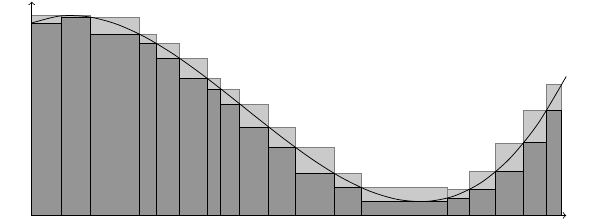
\includegraphics[scale=0.7]{diagrams/riemann}
	\caption[Riemann Integral] {
		A Riemann sum corresponds with the area of a sequence of rectangles.
		Here, the upper and lower Riemann sums for the same partition are shown 
		with light and dark rectangles respectively. 
		A function over an oriented interval is Riemann integrable if the two sums converge.
	\label{fig:riemann}}
\end{figure}


\begin{definition}
The Riemann integral of a function $f:\mathbb{R}^n \to \mathbb{R}$ over a $k$-rectangle 
$[\![\boldsymbol{a}, \boldsymbol{b}]\!]$ as $\max( | \vol( I_{p_1,\ldots, p_n}) | : p_i \in P_i )$ goes to zero.
	\begin{equation}
		\Rie \Big( f,P,\min \big( f(x) \big) \Big) 
		\;\leq\; \int_{[\![a,b]\!]} f(x) \diff x 
		\;\leq\; \Rie \Big( f,P,\max \big( f(x) \big) \Big) 
	\end{equation} 
	If these bounds (upper and lower Riemann sums) converge, we say that a function is \textbf{Riemann integrable} and
	define the Riemann integral as the limit.
\end{definition}





%%%%%%%%%%%%%%%%%%%%%%%%%%%%%%%%%%%%%%%%%
% LEBESGUE INTEGRAL
%%%%%%%%%%%%%%%%%%%%%%%%%%%%%%%%%%%%%%%%%
\section{The Lebesgue Integral on Hybrid Domains}

Another common approach to integration is the Lebesgue integral which approaches integration from a measure theoretic
perspective.
We begin our construction with a $\sigma$-algebra (read sigma-algebra) over a set $X$.
By this we mean a collection of subsets of $X$ which are closed under countable complement, union and intersection.
The important part here is that we have a closed universe of sets on which we can perform 
\emph{nearly} arbitrary set operations but remain within said universe.
Next we can attach to a $\sigma$-algebra a measure to form a \textbf{measure space} $(X, \Sigma, \mu)$ 
where $X$ is a set $\Sigma$ is a $\sigma$-algebra  over subsets of $X$ and $\mu$ is a measure defined on the sets in
 $\Sigma$.
This measure $\mu$ is a function $\mu: \Sigma \to \extendedreal$ with the following properties:
\begin{description}
	\item[Non-negative:] For all $E \in \Sigma$, $\mu(E) \geq 0$
	\item[Empty set has measure 0:] $\mu(\emptyset) = 0$
	\item[Countably Additive:] For $\{E_i\}_i$, a countable set of disjoint sets in $\Sigma$,
		$\mu \left( \bigcup_i E_i \right) = \sum_i \mu(E_i)$
\end{description}
Within the context of integration, the Borel and Lebesgue measure spaces are notable constructions.
Both of which give a suitably large universe of sets for which to integrate over.
Certainly much more than the set of Riemann integrable domains.
Finally, given a measure space $(X, \Sigma, \mu)$, we say that $f : X \to \mathbb{R}$ is a \textbf{measurable function}
if  $\{ x \; | \; f(x) > t\}$ is a measurable set for all $t$.



If $\ind[S]$ is indicator function $\ind[S] : X \to \{ 0, 1 \}$ given by 
$\ind[S] (x) = 1$ if $x \in S$ and $\ind[S] (x) = 0$ otherwise.
Clearly if $S$ is a measurable set, then $\ind[S]$ is a measurable function.
We will use this as a base case.
Given a measure space $(X, \Sigma, \mu)$ and $S \in \Sigma$, we define the integral:
\begin{equation}
	\int \! \ind[S] \diff \mu = \mu ( S )
\end{equation}


From this, we consider functions which are the sum of indicator functions.
We say that $s$ is a \textbf{simple function} if there are finite sets of measurable sets and $\{ A_k \}_{k=0}^n$
and matching real coefficients $\{ a_k \}_{k=0}^n$ such that:
\begin{equation*}
	s = \sum_{k=0}^n a_k \ind[A_k]
\end{equation*}
The integral of a simple function is then easily defined linearly in terms of integrals of indicator functions:
\begin{equation}
	\int \! s \diff \mu 
		= \int \left(\sum_{k=0}^n a_k \ind[A_k] \right) \diff \mu 
		= \sum_{k=0}^n a_k  \int \! \ind[A_k] \diff \mu
		= \sum_{k=0}^n a_k \cdot \mu(A_k)
\end{equation}


But we don't always wish to integrate over the entire measure space but rather some measurable subset of $X$.
This would be done with the notation $\int_B$ instead of $\int$ and replacing $\mu(A_k)$ with $\mu(A_k \cap B)$.
If $A_k$ and $B$ are both measurable sets in $\Sigma$ then their intersection is also a measurable set in $\Sigma$.
But as already mentioned, integrating over sets is a misnomer; we should be integrating over oriented sets.
To do this, we will need to extend $\mu$.


The typical approach would be to construct a \textbf{signed measure} over $\Sigma$.
As a signed measure we lift the non-negative condition and allow for negative values or \emph{charge}.
In one dimension, this is analogous to considering $q-p$ (signed measure) as opposed to Euclidean distance: $||q-p||$ 
(unsigned measure).
But this does not allow us to integrate sets, rather it allows us to integrate sets \emph{with orientation}.
Consider $\int_{[0,1]} \diff\mu$, with no extra information regarding the set $[0,1]$.
This integral is either $1$ or $-1$ we must supply additional information in order to distinguish between 
$\int_0^1 \diff\mu$ and $\int_1^0\diff\mu$.


Instead, both orientation and set are contained within our measurable hybrid sets so we will use this instead.
Rather than a signed measure over the $\sigma$-algebra $\Sigma$ itself, 
we will instead use a signed measure over $\hsetover[\Sigma]$, the space of hybrid sets over $\Sigma$.
Assuming an existing measure $\mu$ on $\Sigma$, this construction comes for free by extending linearly.
Thus, to integrate over a hybrid set $H \in \hsetover[\Sigma]$:
\begin{equation}
	\int_H s \diff \mu = \int H \cdot s \diff \mu = \sum_k a_k \cdot \mu(A_k \otimes H)
\end{equation}


We then use simple functions to approximate general measurable functions.
For a non-negative function $f$, we say this is the largest simple function that is everywhere less than $f$:
\begin{equation}
	\int_H \! f \diff\mu = 
		\text{sup} \left\{ 
			\int_H s \diff \mu \;\middle|\; s \text{ simple, and } 0 \leq \varphi \leq f 
		\right\}
\end{equation}
But even if $f$ takes negative values, we can split it into positive and negative parts by:
\begin{align*}
f^+(x) &:= \mathrm{max}( 0, f(x)) \\
f^-(x) &:= \mathrm{max}(0, -f(x)) 
\end{align*}
Both $f^+$ and $f^-$ are clearly non-negative but also, observe that $f=f^+ - f^-$.
Linearly, this allows us to define for any measurable $f$:
\begin{equation}
\int_H f \diff \mu = \int_H f^+ \diff \mu - \int_H f^- \diff \mu
\end{equation}


The last issue that remains to be settled is whether such a limit of simple functions even exists.
For this we can use the sequence of simple functions $\psi_n$ defined by:
\begin{equation}
	\psi_n = \sum_{k=0}^{n2^n -1} 
		\left[ \left(\frac{k}{2^n}\right)^{\left[ \frac{k}{2^n}, \frac{k+1}{2^n} \right)} \right] 
		+ n^{[n,\infty]}
\end{equation}
Notationally, this definition is rather heavy but is easily understood geometrically as seen below in
Figure~\ref{fig:simplefunc}.
In turn this allows us to define for any non-negative $f$ the sequence of functions:  
\begin{equation}
	\varphi_n = \psi_n \circ f
\end{equation}
We know that $\varphi_n$ is simple since $\psi_n$ is simple.
And since $\psi_n(x) \leq x$ for all $x$ then we also have $0 \leq \varphi_n \leq f$.
But, most importantly we have $0 \leq f(x) - \varphi_n(x) \leq 2^{-n}$ and 
so $\varphi_n$, uniformly approaches $f$ as $n$ approaches infinity. 


\begin{figure}[ht] 
	\centering
	\begin{tikzpicture}[y=1cm, x=2.5cm]
		%psi 4
		\foreach \x in {0,0.0625,...,3.99}
			\draw[fill, color=black!10] (\x,0) rectangle ++ (0.0625, \x);
		\draw[fill, color=black!10] (4,0) rectangle (5,4);
		%psi 3
		\foreach \x in {0,0.125,...,2.9}
			\draw[fill, color=black!20] (\x,0) rectangle ++ (0.125, \x);
		\draw[fill, color=black!20] (3,0) rectangle (5,3);
		%psi 2
		\foreach \x in {0,0.25,...,1.9}
			\draw[fill, color=black!40] (\x,0) rectangle ++ (0.25, \x);
		\draw[fill, color=black!40] (2,0) rectangle (5,2);
		%psi 1
		\foreach \x in {0,0.5,...,0.9}
			\draw[fill, color=black!60] (\x,0) rectangle ++ (0.5, \x);
		\draw[fill, color=black!60] (1,0) rectangle (5,1);
	 	%axis
		\draw(0,0) -- coordinate (x axis mid) (5,0);
	    	\draw (0,0) -- coordinate (y axis mid) (0,5);
	    	%ticks
	    	\foreach \x in {0,1,...,5}
	     		\draw (\x,1pt) -- (\x,-3pt)
				node[anchor=north] {\x};
	    	\foreach \y in {0,1,...,5}
	     		\draw (1pt,\y) -- (-3pt,\y) 
	     			node[anchor=east] {\y}; 
	     	% y= x		
		\draw (0,0) -- (5,5);
		%legend
		\begin{scope}[shift={(5.25,2.5)}] 
			\draw[yshift=4\baselineskip, fill, color=black!60] (0,0) rectangle (0.5,0.2) --++ (0,-0.1)
				node[right, color=black]{$\psi_1$};
			\draw[yshift=3\baselineskip, fill, color=black!40] (0,0) rectangle (0.5,0.2) --++ (0,-0.1) 
				node[right, color=black]{$\psi_2$};	
			\draw[yshift=2\baselineskip, fill, color=black!20] (0,0) rectangle (0.5,0.2) --++ (0,-0.1) 
				node[right, color=black]{$\psi_3$};
			\draw[yshift=\baselineskip, fill, color=black!10] (0,0) rectangle (0.5,0.2) --++ (0,-0.1) 
				node[right, color=black]{$\psi_4$};
			\draw (0,0) -- (0.5,0) node[right] {$id$};
		\end{scope}
	\end{tikzpicture}
	\caption[Approximations using simple functions] {
		The simple functions $\psi_n$ for $n$ from $1$ to $4$.
		As $n$ goes to infinity, $\psi_n$ comes arbitrarily close to $x$ over the range 0 to $n$.
	\label{fig:simplefunc}}
\end{figure}




\pagebreak



%%%%%%%%%%%%%%%%%%%%%%%%%%%%%%%%%%%%%%%%%
% ''HAVING YOUR CAKE AND EATING IT TOO'' EXAMPLE
%%%%%%%%%%%%%%%%%%%%%%%%%%%%%%%%%%%%%%%%%
\subsection{Example: \emph{Integrating the Irrationals}}

A Lebesgue measurable hybrid set can now have an orientation like Riemann integral intervals 
and the power of Lebesgue integration.
Consider the indicator function for the set of rational numbers, $1_\mathbb{Q}$ which evaluates to 
1 for rational numbers and 0 for irrational numbers.
Over the interval $[0,1]$ on the real line, this is not Riemann-integrable.


Suppose we have some generalized partition of $[0,1]$ made up of intervals.
Then for any of these sub-intervals, there will be at least one rational and one irrational number.
Hence the upper Riemann sum will be 1 and the lower Riemann sum will be 0.
No matter how small we make our intervals, there will always be a rational and irrational number in each.
The two sums will never converge and so there is no well-defined Riemann integral.


On the other hand, it is Lebesgue integrable:
\begin{equation*}
	\int_{[0,1]} 1_\mathbb{Q} \diff\mu \;=\; \mu \Big( \mathbb{Q} \cap [0,1] \Big)
\end{equation*}
But since $\mathbb{Q}$ is countable, it has measure 0 and so $1_\mathbb{Q}$ \emph{is} Lebesgue integrable on $[0,1]$.
Similarly, we could also find that:
\begin{equation*}
	\int_0^1 1_{\mathbb{R}\setminus \mathbb{Q}} \diff \mu
		\;=\; \int_{[0,1]} 1_{\mathbb{R}\setminus \mathbb{Q}} \diff \mu
		\;=\; \mu \Big( (\mathbb{R}\setminus\mathbb{Q}) \cap [0,1] \Big)
		\;=\; \mu \Big( (\mathbb{R}\setminus\mathbb{Q}) \cap [0,1] \Big)
		\;=\; 1
\end{equation*}

One would expect the same process to hold for when integrating from 0 to 1 but restricted to sets, this is not possible.
The statement $[1,0] = -[0,1]$ is nonsense.
But if we instead take integrating from $a$ to $b$ to mean the Lebesgue integral over the oriented $[\![a,b]\!]$,
we can get a result of $-1$ as we would expect:
\begin{equation*}
	\int_1^0 1_{\mathbb{R}\setminus \mathbb{Q}} \diff \mu
		\;=\; \int_{[\![1,0]\!]} 1_{\mathbb{R}\setminus \mathbb{Q}} \diff \mu
		\;=\; \mu \big( (\mathbb{R}\setminus\mathbb{Q} ) \otimes [\![1,0]\!] \big)
		\;=\; -\mu \big( (\mathbb{R}\setminus\mathbb{Q} ) \otimes [\![0,1]\!] \big)
		\;=\; -1
\end{equation*}





%%%%%%%%%%%%%%%%%%%%%%%%%%%%%%%%%%%%%%%%%
% DIFFERENTIAL FORMS
%%%%%%%%%%%%%%%%%%%%%%%%%%%%%%%%%%%%%%%%%
\section{Differential Forms}


Rather than thinking of integrals as functions over $n$-rectangles, an often more useful language is to use 
\emph{differential forms}.
We define a \textbf{(differential) 0-form} $\beta$ on $\mathbb{R}^n$ as any function 
$\beta : \mathbb{R}^n \to \mathbb{R}$.
And there is very little else to say as they are just functions on $\mathbb{R}^n$.


A \textbf{(differental) 1-form} $\omega$ on $\mathbb{R}^n$ is an expression of the form:
\begin{equation*}
	\omega = f_1(\text{x}) \diff x_1 + f_2(\text{x}) \diff x_2 + \ldots + f_n(\text{x}) \diff x_n
\end{equation*}
Now this looks very much like something we're used to integrating.
Specifically it is something that be used as an integrand over a 1 dimensional domain.
For example, Green's theorem is often introduced using differential forms 
without even mentioning them as such:
\begin{equation}
	\tag{Green's Theorem}
	\textcolor{black!40}{
		\iint_D \left( \frac{\partial f_2}{\partial x} - \frac{\partial f_1}{\partial y}  \right) \diff x \diff y 
		=\int_{C}
	} \Big( f_1(x,y) \diff x \;+\; f_2(x,y) \diff y \Big)
\end{equation}


Here $C$ is a closed curve that encloses $D$ a region in the $(x,y)$ plane; hence the right-hand side is an integral of
a 1-form over a 1-dimensional curve.
Having multiple $\diff x_i$ appearing in a single integrand may initially seem unusual when first presented, 
but is quite intuitively handled.
Integration is linear so just as we can separate $\int \Big( f(x) + g(x) \Big)\diff x$ into ${\int f(x) \diff x + \int g(x) \diff x}$, 
we can similarly breakup an integral of a 1-form into the sum of integrals over \emph{basic} 1-forms 
(i.e. 1-forms involving only a single term):
\begin{equation*}
	\int \Big( 
			f_1(\text{x}) \diff x_1 
			+ f_2(\text{x}) \diff x_2 
			+ \ldots 
			+ f_n(\text{x}) \diff x_n
		\Big)
	\;=\;	
		\sum_{i=1}^n \left( \int f_i \diff x_i \right)
\end{equation*}


Adding two 1-forms then is quite straight-forward; simply collect terms with matching $\diff x_i$.
So if we can add differential forms but what about multiplication?
For a 0-form $\beta$ and 1-form $\omega$ as defined above, the answer the answer is a simple yes:
\begin{equation*}
	(\beta \cdot \omega)(\text{x}) 
		= \Big( \beta(\text{x})f_1(\text{x}) \Big) \diff x_1
		+ \ldots  
		+ \Big( \beta(\text{x})f_n(\text{x}) \Big) \diff x_n
\end{equation*}
The result is a 1-form where each basic 1-form term is the product of $f_i$ and $\beta$ in $\mathbb{R}$.
To ``multiply'' two 1-forms together however we must turn instead to the wedge product $\wedge$.


First of all, the wedge product is primarily defined by being \emph{anti-commutative} or \emph{skew-symmetric}.
That is, $\diff x \wedge \diff y = -\diff y \wedge \diff x$ and several results will immediately follow.
When applied to two identical $\diff x$, we have $\diff x \wedge \diff x = - \diff x \wedge \diff x$ 
and so $\diff x \wedge \diff x = 0$.
Additionally, for any permutation $\sigma$ of $[p]$:
\begin{equation*}
	\diff x_1 \wedge ... \wedge \diff x_p 
	= \text{sgn}(\sigma) \diff x_{\sigma(1)} \wedge ... \wedge \diff x_{\sigma(p)}
\end{equation*}
The wedge product of two 1-forms moves us out of the realm of 1-forms which have basis $\diff x_i$ and into the 
realm of 2-forms with basis $\diff x_i \wedge \diff x_j$.


\begin{definition}
	Given a $k$-rectangle $\Omega \in \mathbb{R}^n$ with coordinates $\text{x} = (x_1, x_2, \ldots, x_n)$
	A \textbf{differential $p$-form} $\beta$ over $\Omega$ has the form:
	\begin{equation}
		\beta = \sum_{j_1 \in [n]} \ldots \sum_{j_p \in [n]} 
			\Big( 
				b_{(j_1, \ldots, j_p)}(\text{x})
				\diff x_{j_1} \wedge \ldots \wedge \diff x_{j_p}
			\Big)
	\end{equation}
	Typically, we will take $j$ to be the vector $(j_1, \ldots, j_p)$ 
	and express $\beta$ instead as a single sum multi-indexed
	by $j$.
	We denote the \textbf{space of all $\boldsymbol{p}$-forms on $\boldsymbol{\Omega}$} as $\Lambda^p(\Omega)$.
\end{definition}

\begin{definition}
	Let $\alpha = \sum_i a_i(x) \diff x_{i_1} \wedge \ldots \wedge \diff x_{i_p} \in \Lambda^p(\Omega)$ 
	and $\beta = \sum_j b_j(x) \diff x_{j_1} \wedge \ldots \wedge \diff x_{j_q} \in \Lambda^q(\Omega)$. 
	We extend the wedge product to 
	$\wedge : \Lambda^p(\Omega) \times \Lambda^q(\Omega) \to \Lambda^{p+q}(\Omega)$ by:
	\begin{equation}
		\alpha \wedge \beta  = \sum_{i,j}  \Big( a_i(x) b_j(x) \;
			\diff x_{i_1} \wedge \ldots \wedge \diff x_{i_p} \wedge 
			\diff x_{j_1} \wedge \ldots \wedge \diff x_{j_q}
			\Big)
	\end{equation}
\end{definition}


Although we take all possible $\binom{n}{q} \cdot \binom{n}{p}$ pairs of 
$a_i (x) \diff x_{i_1} \wedge \ldots \wedge \diff x_{i_p}$ and $b_i (x) \diff x_{i_1} \wedge \ldots \wedge \diff x_{i_p}$,
most of the possible terms will end up being zero.
If \emph{any} of the terms in $\diff x_{i}$ appears in $\diff x_{j}$, then the wedge product will be zero 
and no term will be contributed.
As such, if $q+p > n$, there will be a duplicate in every term and so the entire sum will be zero.
When all is said and done, at most we will have $\binom{n}{p+q}$ terms.
Rather than the skew-symmetry we had when commuting $\diff x \wedge \diff y$, 
in higher dimensions the sign depends on $p \cdot q$ of the $p$-form and $q$-form we are commuting.
Specifically, 
\begin{equation} 
	\label{eqn:wedgetranspose}
	\alpha \wedge \beta = (-1)^{pq} \beta \wedge \alpha
\end{equation}
This can be easily seen by commuting each of $\diff x_{j_1}, \ldots \diff x_{j_q}$ terms each past 
$\diff x_{i_1}\wedge \ldots \wedge \diff x_{i_p}$. 
So we are commuting $q$ terms each past $p$ terms, reversing the sign each time for a net $(-1)^{pq}$.
This result generalizes the earlier skew-symmetry of transposing $\diff x \wedge \diff y$.
When $\alpha$ and $\beta$ are both 1-forms then clearly $-1^{pq} = -1^{1\cdot1}= -1$.


The wedge product is only one part of our algebra of differential forms.
We have several other nice identities for its behaviour with addition and multiplication.
For the following, we consider $f$ to be a function on $\mathbb{R}^n$.
Additionally we consider the differential forms $\omega_1$ and $\omega_2$ to be $k$-forms, 
$\alpha$ to be a $p$-form and $\beta$ to be an $q$-form.
Then we have the following:
\begin{align}
	(\omega_1 + \omega_2) \wedge \alpha  & \;=\; \omega_1 \wedge \alpha + \omega_2 \wedge \alpha \\
	(\omega_1 \wedge \alpha) \wedge \beta & \;=\; \omega_1 \wedge ( \alpha \wedge \beta ) \\
	(f \cdot \omega_1) \wedge \alpha & \;=\;  f \cdot (\omega_1 \wedge \alpha) \;=\; \omega_1 \wedge (f \cdot \alpha)
\end{align}
These should all be quite obvious from definitions. 
We should also note the identities which are \emph{not} present.
We have defined the sum of $\omega_1$ and $\omega_2$: two differential forms which are the same dimension but not
the sum of $\alpha$ and $\beta$: differential forms with different dimension.
It is clear how one would add two differential forms of the same dimension as both were defined as sums to begin with.
We also do not define the multiplication of $\cdot$ two differential forms but we multiplying a form by a function is simply:
\begin{equation*}
	(f \cdot \alpha) (x) = \sum_i f(x)\cdot a_i(x) \diff x_{i_1} \wedge \ldots \wedge \diff x_{i_p}
\end{equation*}


Integrating over a $k$-form is quite simple.
First, consider integrating a $k$-form over a $k$-rectangle in $\mathbb{R}^k$.
Such a $k$-form is also known as a \emph{top-dimensional form}.
As we saw previously, any form of higher degree must be zero.
If $\omega$ is such a top form then we can always write
\begin{equation*}
	\omega = f \; \diff x_1 \wedge \ldots \wedge \diff x_k
\end{equation*}
for some function $f$.
Other presentations of $\omega$ exist, but we can always achieve such a presentation by commuting over $\wedge$ 
to the canonical ordering $x_1, \ldots, x_n$.
Once a $k$-form in this presentation, remove the wedges and evaluate the integral using the
integrand $f \diff x_1 \diff x_2 \ldots \diff x_k$.


\begin{definition}
	Let $\alpha$ be a $k$-form on $\Omega \subset \mathbb{R}^n$ of the form 
	$\alpha = A(x) \diff x_1 \wedge ... \wedge \diff x_n$.
	If $A \in \mathcal{L}^1 (\Omega , \diff x)$ then we define:
	\begin{equation}
		\int_\Omega \alpha = \int_\Omega A(x) \; \diff x
	\end{equation}
	Where the left-hand side is the integral of a $k$-form and the right-hand side is a Lebesgue integral.
	For any $\beta \in \Lambda^k (\Omega)$ we extend this definition linearly as the sum of integrals.
\end{definition}


Finally, we extend the differential operator $\diff$ to act on forms known as the \textbf{exterior derivative}.
For a function (0-form), it is the 1-form:
\begin{equation}
	\diff f = \sum_i \frac{\partial f}{\partial x_i} \diff x_i
\end{equation}
This will result in equivalent 1-forms regardless of the choice of coordinates $\text{x} = (x_1, \ldots, x_n)$.
For higher dimension forms it will similarly map a $k$-form to a $k+1$-form.
This is done by recursively using the identities for $p$-form $\alpha$ and $q$-form $\beta$.
\begin{align}
	\diff (\alpha \wedge \beta) &= (\diff \alpha) \wedge \beta + (-1)^p \alpha \wedge ( \diff \beta) \\
	\diff (\;\diff ( \alpha )\; ) &= 0
\end{align}
and extending linearly for all $k$-forms.





%%%%%%%%%%%%%%%%%%%%%%%%%%%%%%%%%%%%%%%%%
% SINGULAR CUBE
%%%%%%%%%%%%%%%%%%%%%%%%%%%%%%%%%%%%%%%%%
\section{Singular Cubes}


Up until now we have been dealing with the very small set of axis aligned $k$-rectangles 
which is a very limiting class to be restricted to.
Instead we would like to be able to integrate over $k$-rectangles that are deformed by some smooth function.
So assume that we have $X \subset \mathbb{R}^m$ and $Y \subset \mathbb{R}^n$ and a smooth map 
 $\varPhi : X \to Y$.
Not only can we map points from $X$ to points in $Y$ but we can \emph{push foward} vectors from $X$ to vectors in $Y$
and with them, push forward tangent spaces as well.


\begin{definition}
	We denote the \textbf{standard $\boldsymbol{k}$-cube} as the specific $k$-rectangle $[\![0,1]\!]^k$ in 	
	$\mathbb{R}^n$ which is the Cartesian product of $k$ copies of $[\![0,1]\!]$.
	We also consider $[\![0,1]\!]^0 = \{0\}$.
	Given an $k$-dimensional manifold $M$, a \textbf{singular $\boldsymbol{k}$-cube in $\boldsymbol{M}$} is a 
	smooth differentiable map $c$ from the standard $k$-cube to $M$, $c:[\![0,1]\!]^k \to M$.
	We will abuse this notation somewhat by also using $c \subseteq M$ to refer to the image of $[\![0,1]\!]^k$ under $c$.
\end{definition}


For example, the hemisphere $H = \{ (x,y) \; | \: x \geq 0, y\geq 0, x^2+y^2 \leq 1 \}$
is a singular 2-cube under the transformation $c: (r, \varphi) \mapsto r \cos(\pi \varphi) x+ r \sin(\pi \varphi) y$.
Depending on the context we might refer to either $H$ or $c$ as a singular cube.
Also, the choice of using specifically the standard $k$-cube is arbitrary.
A differentiable map $f$ from $[\![a,b]\!]$ can always be composed with $g:t \mapsto ta +(1-t)b$ 
to construct the singular cube $c=f \circ g$.


However if we have a valid integral $\int_{\Omega} \omega$ with $\Omega$ in some space $X$, 
if we push forward $\Omega$ by some function $c$ to another space $Y$, 
then the integral $\int_{c(\Omega)} \omega$ is no longer valid.
The differential form $\omega$ was expressed in coordinates for $X$ but now that the domain of the integral is in $Y$,
we must perform a change of coordinates.
The true reason why we use differential forms is how cleanly they handle this change in coordinates 
through the use of pull-backs.


Informally, a pullback is a \emph{reversed} function composition.
In typical function composition $(f \circ g)(x) = f(g(x))$, for input $x$ one first evaluates the second function $g$ at $x$
before feeding the result of $g(x)$ into the first function $f$.
The pre-composition or pullback would be $f^*g = g(f(x))$. 
One first evaluates the first function and feeds the result into the second.
Gets its name from pulling $f$ back through $g$.
Using the following identities:
\begin{align}
	F^* (\alpha \wedge \beta ) &= (F^* \alpha) \wedge (F^* \beta) \\
	F^* (\diff \beta ) &= \diff F^* \beta
\end{align}
one finds a very convenient way to express change of basis inside an integral.


\begin{theorem}
Let $F : X  \to \Omega$ be an (orientation-preserving diffeomorphism) and $\alpha$ an integrable $n$-form on $\Omega$ then
\begin{equation}
\int_{F(X)} \alpha = \int_X F^* \alpha
\end{equation}
\end{theorem}


To integrate over a manifold $M$, we first observe that each local chart $U_i$ in the manifold is essentially a singular cube.
If the chart is not a map over the standard cube, then there exists a diffeomorphism 
that can be composed with the local map to transform it into a singular cube.
It is then a matter of stitching together these local charts so that points in the manifold are not ``double-counted''.
To do this we use a \textbf{partition of unity} on $M$.
That is, a collection of functions $\{ \psi_i \}_i$, $\psi_i: U_i \to \mathbb{R}$ which is:
\begin{description}
	\item[Non-negative:] For each $\psi_i$ and for all $x \in \text{supp}(\psi_i)$, $\psi_i \geq 0$ .
	\item[Sums to one(unity):] For all $x \in M$, $\sum_i \psi_i(x) = 1$
	\item[Locally finite:] for any point in $M$ there are only a finite number of non-zero $\psi_i$
\end{description}
Given such a parititon of unity for the manifold, we define the integral over all of $M$ as:
\begin{equation}
\int_M \alpha = \sum_i \int_{U_i} \psi_i \alpha
\end{equation}









\chapter{Convolution of Piecewise-defined Functions}

Convolution is an operation which takes two functions and produces a third.
It takes one of the two input functions, and modifies one by mirroring and translating.
The resulting function is then the overlap between one of these functions as a function of the translation.
Visually, this can be seen below in Figure~\ref{fig:ConvolutionExample}.

\begin{figure}[ht]
	\caption[Convolution of box signal with itself]{The convolution of the box signal 
	$f(t)=g(t)=\left( 0^\oiOpOp{-\infty,-0.5} \oplus 1^\oiClCl{-0.5,0.5} \oplus 0^\oiOpOp{0.5,\infty} \right)$ with itself.
	\label{fig:ConvolutionExample}}
	\centering
	\begin{tikzpicture}[scale=3.8]
		\draw[fill, color=black!10] (-1.75,1.5) rectangle (-1.4,2);	
		\draw[fill, color=black!10] (-0.25,1.5) rectangle (0.25,2);	
		\draw[fill, color=black!10] (1.75,1.5) rectangle (1.7,2);	
	
		\draw[<->] (-2,0) -- (2,0);
		\draw[<->] (0,-.1) -- (0,1.1);
		\draw[very thick] (-2,0) -- (-1,0) -- (0,1) -- (1,0) -- (2,0);
			
			
		\draw[<->] (-2,1.5) -- (-1,1.5);
		\draw[<->] (-1.5,1.4) -- (-1.5, 2.1);
		\draw[dashed, <->] (-1.65,1.4) -- (-1.65, 2.1);
		
		\draw[<->] (-.5,1.5) -- (.5,1.5);
		\draw[<->] (0,1.4) -- (0, 2.1);
		\draw[dashed, <->] (-0.01,1.4) -- (-0.01, 2.1);
		
		\draw[<->] (1,1.5) -- (2,1.5);
		\draw[<->] (1.5,1.4) -- (1.5, 2.1);
		\draw[dashed, <->] (1.95,1.4) -- (1.95, 2.1);
		
		
		\draw[thick] (-2,1.5) -- (-1.75,1.5) -- (-1.75,2) -- (-1.25,2) -- (-1.25,1.5) -- (-1,1.5);
		\draw[thick,dashed] (-2,1.5) -- (-1.9,1.5) -- (-1.9,2) -- (-1.4,2) -- (-1.4,1.5) -- (-1,1.5);
		
		\draw[thick] (-.5,1.5) -- (-.25,1.5) -- (-.25,2) -- (.25,2) -- (.25,1.5) -- (.5,1.5);
		\draw[thick,dashed] (-.5,1.51) -- (-.255,1.51) -- (-.255,2.01) -- (.245,2.01) -- (.245,1.51) -- (.5,1.51);
		
		\draw[thick] (2,1.5) -- (1.75,1.5) -- (1.75,2) -- (1.25,2) -- (1.25,1.5) -- (1,1.5);
		\draw[thick,dashed] (2,2) -- (1.7,2) -- (1.7,1.5) -- (1,1.5);


		\draw[dashed] (-0.01,1.3) -- (-0.01,-.1) node [below] {$t=0$};
		\draw[dashed] (-1.65,1.3) -- (-1.65, 1) -- (-0.4, 0.5) -- (-0.4,-.1) node [below] {$t=-0.4$};
		\draw[dashed] (1.95,1.3) -- (1.95, 1) -- (0.9,0.5) -- (0.9,-.1) node [below] {$t=0.9$};
		
	\end{tikzpicture}
\end{figure}

Formally this, equates to the following definition for convolution over continuous domains:
\begin{definition}
	The \textbf{convolution} $*$, of two functions $F$ and $G$ is defined as:
	\begin{equation}
		(F*G)(t) = \int_{-\infty}^\infty F(\tau) \;G(t - \tau) \; d\tau
	\end{equation}
\end{definition}
and in the case of discrete linear convolution, summation would replace integration.
In this equation, $t$ represents the translation of $G$ as well as the input for $(F*G)$
while $\tau$ is internal to the integral and varies over the real line.


\begin{figure}[ht]
	\caption[Gaussian Blurring]{512x512px ``Lena''(a) with a 1px (b) and 5px (c) Gaussian blur applied. 
	Gaussian blurring is accomplished by convolving an image with a Gaussian kernel and is commonly used
	in image processing to reduce noise prior to edge detection.
	\label{fig:LenaBlur}}
	\centering
	\begin{subfigure}[b]{0.3\textwidth}
                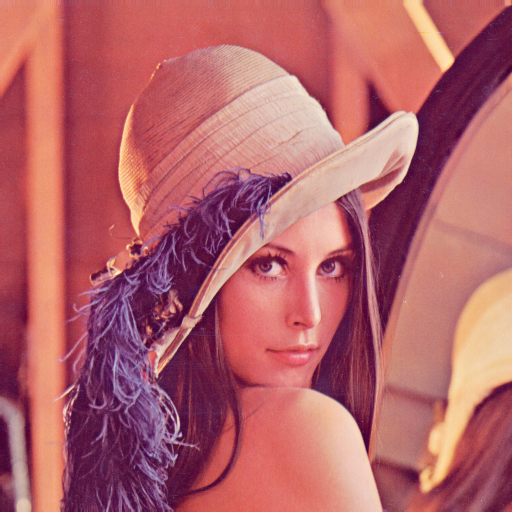
\includegraphics[scale=0.25]{diagrams/Lenna}
                \caption{Original Image}
       \end{subfigure}
       \begin{subfigure}[b]{0.3\textwidth}
                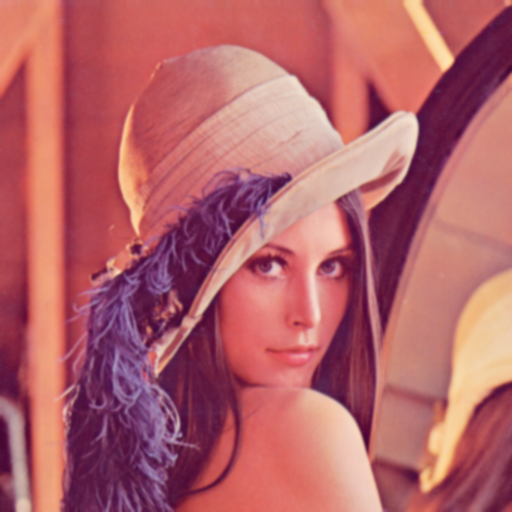
\includegraphics[scale=0.25]{diagrams/Lenna-blur1}
                \caption{1px Gaussian blur}
       \end{subfigure}
       \begin{subfigure}[b]{0.3\textwidth}
                
\includegraphics[scale=0.25]{diagrams/Lenna-blur5}
                \caption{5px Gaussian blur}
       \end{subfigure}
\end{figure}


Convolution has applications in many areas of mathematics and engineering.
One very common use in image processing is in blurring.
\emph{Gaussian blurring} is the result of a convolution in 2-dimensions of an image with the Gaussian distribution function:
\begin{equation}
	\label{eqn:2dGaussian}
	G(x,y) = \frac{1}{2 \pi \sigma^2} \; \text{exp} \left( - \frac{x^2 + y^2}{2\sigma^2} \right)
\end{equation}
Blurring an image in this way reduces noise and greatly increases the efficacy of subsequent edge detection.
In statistics, a (simple) \emph{moving average} can be represented as a convolution by a rectangular pulse while more
generally, weighted moving averages can be made by convolving with other functions.





%%%%%%%%%%%%%%%%%%%%%%%%%%%%%%%%%%%%%%%%%
%
% CONVOLUTION OF PIECEWISE
%
%%%%%%%%%%%%%%%%%%%%%%%%%%%%%%%%%%%%%%%%%
\section{Convolution of Piecewise Functions}\label{sec:PWConvolution}


CAS such as Maple and Mathematica are quite adept at solving integrals.
Convolution of elementary functions generally poses no problem.
When convolving two piecewise continuous functions, many possible intervals arise and the conditionals that arise
can quickly overwhelm them unaided.


We are interested in \emph{Symbolic Linear Convolution} (of piecewise continuous functions).
The typical approach is to first consider for convolution of ``one piece'' functions 
\cite{evans1994algorithms, west1993symbolic}.
By ``one-piece'' functions we mean functions which are restricted to a single interval and zero everywhere else.
We will consider two functions, $F$ and $G$ defined as:


\begin{equation}
	\label{eqn:fOnePiece}
	F(x)=f^{[a_f,b_f)}(x) = 
		\begin{cases}
			f(x) & a_f \leq x < b_f \\
			0 & \text{otherwise}
		\end{cases}
\end{equation}
\begin{equation}
	\label{eqn:gOnePiece}
	G(x)=g^{[a_g,b_g)}(x) = 
		\begin{cases}
			g(x) & a_g \leq x < b_g \\
			0 & \text{otherwise}
		\end{cases}
\end{equation}
for which we would like to compute the convolution $(F*G)$.
To reduce the total number of cases generated, it is generally also assumed that $b_f - a_f \leq b_g - a_g$.
Assuming that $F$ is non-zero over a shorter interval is not that strong an assumption as convolution is commutative;
if it is not the case we can rearrange $F*G$ to $G*F$.
To see this, simply apply the substitute $\tau' = t-\tau$ in equation (7.1):
\begin{align}
	\label{eqn:ConvCommutative}
	(F*G)(t) 
		&= \int_{-\infty}^\infty F(\tau) G(t-\tau) \;d \tau 
		\notag\\&= \int_{\infty}^{-\infty} F(t-\tau')G(\tau')\; (-1) d\tau' 
		\notag\\&= \int_{-\infty}^\infty G(\tau') F(t-\tau') \; d\tau'
		\notag\\&= (G*F)(t)
\end{align}


Thus we can assume that our static function is also the function with the shorter interval.
Since $F$ and $G$ are zero outside of their respective intervals, we do not need to integrate over the entire real line. 
$F$ is our static function, so $[a_f, b_f)$ would be sufficient.
For a tight boundary, we have the following:
\begin{align}
	\label{eqn:ConvNaiveOnePiece}
	(F*G)(t) 
	&= \int_{-\infty}^\infty F(\tau)\; G(t-\tau) \; d\tau \notag \\
	&= \int_{a_f}^{b_f} f(\tau) \; G(t-\tau) \; d\tau \notag \\
	&= 	\begin{cases}
			\int_{a_f}^{t-a_g} f(\tau) \; g(t-\tau) \; d\tau 	& (a_f+a_g) \leq t < (b_f+a_g) \\
			\int_{a_f}^{b_f} f(\tau) \; g(t-\tau) \; d\tau		& (b_f+a_g) \leq t < (a_f+b_g) \\
			\int_{t-b_g}^{b_f} f(\tau) \; g(t-\tau) \; d\tau	& (a_f+b_g) \leq t < (b_f+b_g) \\
			0										& \text{otherwise}
		\end{cases}
\end{align}


\begin{figure}[ht]
	\caption[Convolution of ``one-piece'' functions]{Convolution of length 1 and 2 rectangular pulses. 
	Given the functions $F=1^{[-1,1)}$ and $G=1^{[-2,2)}$, there are three non-zero regions in $(F*G)$.
	\label{fig:OnePiece}}
	\centering
	\begin{tikzpicture}
		\begin{axis}[
			x=1.5cm,
			y=1.5cm,
			xstep=1,
			ystep=1,
			xmin=-3.9,xmax=3.9,
			ymin=-0.4,ymax=2.4,
			axis x line=middle,
			axis y line=middle,
			axis line style=<->,
			xlabel={$x$},
			ylabel={$y$},
	        ]
		\addplot[no marks,black,very thick,<-] expression[domain=-3.9:-3,samples=100]{0};
		\addplot[no marks,black,very thick,-] expression[domain=-1:1,samples=100]{2};
		\addplot[no marks,black,very thick,-] expression[domain=-3:-1,samples=100]{x+3};
		\addplot[no marks,black,very thick,-] expression[domain=1:3,samples=100]{3-x};
		\addplot[no marks,black,very thick,->] expression[domain=3:3.9,samples=100]{0};
		\node(afag) at (axis cs:-3,2.25) {$a_f+a_g$};
		\node(bfag) at (axis cs:-1,2.25) {$b_f+a_g$};
		\node(afbg) at (axis cs:1,2.25) {$a_f+b_g$};
		\node(bfbg) at (axis cs:3,2.25) {$b_f+b_g$};
	        \end{axis}
		%\draw[thick,<->] (-4,0) -- (4,0);
		%\draw[thick,<->] (0,-.5) -- (0,1.5);
		
	\end{tikzpicture}
\end{figure}


These regions can be visualized as above in Figure~\ref{fig:OnePiece} where two rectangular pulses are convolved. 
If both functions had equal length non-zero intervals (i.e. $b_f-a_f = b_g-a_g$), then the central plateau would be empty
(as in Figure~\ref{fig:ConvolutionExample}).
Another formulation presented by C\^{i}rnu \cite{cirnu2012calculation} and Cavicchi \cite{cavicchi2002simplified} is to use:
\begin{equation}
	\label{eqn:ConvCirnu}
	(F*G)(t)=
	\begin{cases}
		\int_{\max(a_f, \; t-b_g)}^{\min(b_f, t-a_g)} f(\tau)\cdot g(t-\tau)\; d\tau & (a_f+a_g) \leq t < (b_f+b_g) \\
		0 & \text{otherwise}
	\end{cases}
\end{equation}
Although this may appear to reduce the number of cases, expanding the $\min$ and $\max$ will cause just as many 
cases to return.


To extend this to piecewise continuous function, 
we simply treat each piecewise function as the sum of ``one-piece'' functions.
Given functions, $F= \sum_i f_i^{P_i}$ and $G= \sum_j g_j^{Q_j}$ 
where $\{P_i\}$, $\{Q_j\}$ are each sets of disjoint intervals, and $f_i^{P_i}$, $g_j^{Q_j}$ are all ``one-piece'' functions.
The convolution of $F*G$ is the sum of pairwise convolution:

\begin{align}
	\label{eqn:ConvPiecewise}
	\left(\left(\sum_i f_i^{P_i}\right) * \left(\sum_j g_j^{Q_j}\right)\right) (t)
	&= \int_{-\infty}^\infty \left(\sum_i f_i^{P_i}\right)(\tau)\cdot \left(\sum_j g_j^{Q_j}\right)(t-\tau) \;d\tau
	\notag\\&= \sum_i \sum_j \int_{-\infty}^\infty f_i^{P_i}(\tau) \cdot g_j^{Q_j}(t-\tau) \;d\tau 
	\notag\\&= \sum_i \sum_j \left(f_i^{P_i} * g_j^{P_j}\right)
\end{align}

To summarize, the algorithm for convolution of two piecewise functions is as follows:
\begin{enumerate*}
	\item Each function is converted into a sum of disjoint function intervals.
	\item Each function interval in one function is convolved with each function interval in the other.
	\item The final result is the sum of all function interval convolutions.
\end{enumerate*}


This is the typical approach to convolution of piece-wise functions as presented by West and McClellan  
\cite{west1993symbolic}.
When the boundaries between regions is symbolic, then we may not be able to determine which interval is longer.
Another approach involving hybrid functions will be presented in Section~\ref{sec:HFConvolution}. 
Concerns with intervals where one boundary point is at infinity have also been raised \cite{evans1994algorithms}.
Techniques to handle this will be investigated in Section~\ref{sec:ConvInfty}.








%%%%%%%%%%%%%%%%%%%%%%%%%%%%%%%%%%%%%%%%%
%
% HYBRID CONVOLUTION
%
%%%%%%%%%%%%%%%%%%%%%%%%%%%%%%%%%%%%%%%%%
\section{Hybrid Function Convolution}
\label{sec:HFConvolution}

Our exposition for hybrid set convolution will appear very similar to that from the previous section and can be seen as a
 replacement for step 2 in the algorithm.
Again we will be interested in the convolution of ``one-piece'' functions which we will use to build up piece-wise
continuous functions.
Assuming two hybrid one-piece functions $f^{[a_f, b_f)}$ and $g^{[a_g,b_g)}$ which are 0 outside of the intervals
 $[a_f,b_f)$ and $[a_g, b_g)$ respectively.
Then the \textbf{hybrid convolution of $\boldsymbol{f^{[a_f,b_f)}}$ and $\boldsymbol{g^{[a_g,b_g)}}$} is:
	\begin{align}
		\label{eqn:defHConvolution}
		(f^{[a_f,b_f)} \;*\; g^{[a_g,b_g)}) (t) = 
			\R[+] &\left( \; \left( 
				\int_{[\![a_f,\;t-a_g)\!)} f(\tau) \; g(t-\tau) \; d\tau \right)^{[\![a_f+a_g,\; b_f+a_g)\!)} 
					\right. \notag \\ &\oplus \left( 
				\int_{[\![a_f,\;b_f)\!)} f(\tau) \; g(t-\tau) \; d\tau \right)^{[\![b_f+a_g,\; a_f+b_g)\!)} 
					\notag \\ &\oplus \left. \left( 
				\int_{[\![t-b_g,\;b_f)\!)} f(\tau) \; g(t-\tau) \; d\tau \right)^{[\![a_f+b_g,\; b_f+b_g)\!)} 
					\; \right)(t)
	\end{align}

The first thing one should note is the similarity between this expression and (\ref{eqn:ConvNaiveOnePiece}).
But, \emph{we do not enforce} $b_f - a_f \leq b_g - a_g$ as we did in Section~\ref{sec:PWConvolution}.
Instead both cases will be handled by our generalized partition structure.
If the integral $f(t)g(t-\tau)$ is is easier to compute than $g(t)f(t-\tau)$ then the convolution can, of course, 
still be commuted.
This could be due to the nature of functions for $f$ and $g$ or if $f$ and $g$ are a part of a larger sum with identical 
sub-functions on different regions.
Then these integrals could potentially be combined, provided they have the same integrand, resulting in fewer overall 
integrals to compute.
The ordering of $f$ and $g$ is no longer dictated by the relative length of their respective intervals.


When $b_f - a_f \leq b_g - a_g$ then the three oriented intervals will be disjoint and the two equations are identical.
Otherwise, if $b_f - a_f > b_g - a_g$, then the interval $[\![b_f +a_g, \; a_f + b_g)\!)$ will have a negative orientation.
The intervals $[\![a_f+a_g, \; b_f+a_g)\!)$, $[\![b_f+a_g, \; a_f+b_g)\!)$ and $[\![a_f+b_g, \; b_f+b_g)\!)$ still forms
a reducible (i.e. everywhere multiplicity one) generalized partition over $[a_f+a_g, \; b_f+b_g)$.
Outside this region the function is zero as expected. 

\pagebreak

Suppose we are in this second case and we wish to evaluate the convolution at a point $t$ which is in all three intervals.
This occurs when $(a_f+b_g) \leq t < (b_f+a_g)$ and we have:
\begin{align*}
	[\![a_f+a_g, \; b_f+a_g)\!)(t) &= 1 \\
	[\![b_f+a_g, \; a_f+b_g)\!)(t) &= -1 \\
	[\![a_f+b_g,\; b_f+b_g)\!)(t) &= 1
\end{align*}
Simplifying the $+$-reduction we then get:
\begin{align}
	(f^{[a_f,b_f)} \;*\; g^{[a_g,b_g)}) (t) = 
		& \; \left( 
			\int_{[\![a_f,\;t-a_g)\!)} f(\tau) \; g(t-\tau) \; d\tau \right) 
				\notag \\ &- \left( 
			\int_{[\![a_f,\;b_f)\!)} f(\tau) \; g(t-\tau) \; d\tau \right)
				\notag \\ &+ \left( 
			\int_{[\![t-b_g,\;b_f)\!)} f(\tau) \; g(t-\tau) \; d\tau \right) 
\end{align}
All three of these integrals have the same integrand so we can use bi-linearity to move the sum to be over the domains
of integration.
These domains then cancel nicely to leave us with:
\begin{align}
	\label{eqn:HybridConvMidFinal}
	(f^{[a_f,b_f)} \;*\; g^{[a_g,b_g)}) (t) = &
		\int_{[\![a_f,\;t-a_g)\!) \;\ominus\; [\![a_f,\;b_f)\!) \;\oplus\; [\![t-b_g,\;b_f)\!)} f(\tau) \; g(t-\tau) \; d\tau \notag\\
		= & \int_{[\![t-b_g,\;t-a_g)\!)} f(\tau) \; g(t-\tau) \; d\tau
\end{align}
Let us now look at a concrete example with some actual numbers.





%%%%%%%%%%%%%%%%%%%%%%%%%%%%%%%%%%%%%%%%%
% HYBRID EXAMPLE
%%%%%%%%%%%%%%%%%%%%%%%%%%%%%%%%%%%%%%%%%
\subsection{Example: \emph{Hybrid Convolution}}


In Figure~\ref{fig:OnePiece} we saw the convolution of $1^{[-1,1)}$ with $1^{[-2,2)}$.
We know that convolution is commutative so computing $1^{[-2,2)} * 1^{[-1,1)}$ we already know what to expect.
We will label these as $1_f$ and $1_g$ to differentiate and to prevent confusion by reminding us that the object we are 
dealing with is $x \mapsto 1$ rather than the number 1 itself.

\begin{align}
	\label{HCExample}
	(1_f^{[-2,2)} \;*\; 1_g^{[-1,1)}) (t) = 
		\R[+] &\left( \; \left( 
			\int_{[\![-2,\;t-1)\!)} f(\tau) \; g(t-\tau) \; d\tau \right)^{[\![-3,\; 1)\!)} 
				\right. \notag \\ &\oplus \left( 
			\int_{[\![-2,\;1)\!)} f(\tau) \; g(t-\tau) \; d\tau \right)^{[\![1,\; -1)\!)} 
				\notag \\ &\oplus \left. \left( 
			\int_{[\![t-1,\;2)\!)} f(\tau) \; g(t-\tau) \; d\tau \right)^{[\![-1,\; 3)\!)} 
				\; \right)(t)
\end{align}


Already this is promising as we can see the set of end-points: $\{-3, -1, 1, 3\}$ agrees with our previous example.
Let us consider three points $t_1 \in [-3, -1)$, $t_2 \in [-1, 1)$ and $t_3 \in [1,3)$.
We omit the derivations but encourage the reader to convince themselves that each is correct.
\begin{equation*}
	(1_f^{[-2,2)} \;*\; 1_g^{[-1,1)}) (t_1) 
		\;=\; \int_{[\![-2,\;t_1-(-1))\!)} 1_f(\tau) \; 1_g(t_1-\tau) \; d\tau
		\;=\; t_1 + 3
\end{equation*}
First we should note that at no point in the integral do we attempt to evaluate $1_f$ or $1_g$ outside of their original 
domains $[-2,2]$ and $[-1,1]$ respectively. 
Thus it is safe to replace $1_f(\tau)\cdot 1_g(t-\tau)$ with 1  inside the integral.
From here, the integral is trivially evaluated and is as expected.


For $t_3$, only the third term has non-zero multiplicity and by an identical argument as for $t_1$ we have:
\begin{equation*}
	(1_f^{[-2,2)} \;*\; 1_g^{[-1,1)}) (t_3) 
		\;=\; \int_{[\![t-1,2)\!)} 1_f(\tau) \; 1_g(t_3-\tau) \; d\tau
		\;=\; 3 - t_3
\end{equation*}
Finally, $t_2$ deviates from this pattern slightly as $t_2$ is in \emph{all three} oriented intervals.
By the same derivation as we used in the previous section we can use equation~(\ref{eqn:HybridConvMidFinal}):
\begin{equation*}
	\label{eqn:HCExampleT2}
	(1_f^{[a_f,b_f)} \;*\; 1_g^{[a_g,b_g)}) (t_2) 
		\;=\; \int_{[\![t_2-1,\;t_2-(-1))\!)} f(\tau) \; g(t-\tau) \; d\tau
		\;=\; 2
\end{equation*}
For any other point $t$ which is not in $[-3, 3)$, then all three oriented intervals will have multiplicity zero.
Simplifying the $+$-reduction we have, $\R[+](\emptyset) = e_+ = 0$ and so (\ref{HCExample}) evaluates correctly 
everywhere.





%%%%%%%%%%%%%%%%%%%%%%%%%%%%%%%%%%%%%%%%%
%
% INFINITE INTERVALS
%
%%%%%%%%%%%%%%%%%%%%%%%%%%%%%%%%%%%%%%%%%
\section{Infinite Intervals}\label{sec:ConvInfty}


The method presented in Section \ref{sec:PWConvolution} behaves correctly assuming that all the end points are finite.
But Evans and McClellan \cite{evans1994algorithms} raise two issues that arise when we allow for interval end points at
infinity. Namely,
\begin{enumerate*}
	\item Interval lengths can no longer be compared to ensure the first interval is shorter than the second.
	\item Indeterminant arithmetic may occur in computing new endpoints of the form $+\infty-\infty$
\end{enumerate*}


We have already shown that hybrid function convolution is not concerned with the relative length of functions. 
Clearly, the first point should not be a concern for hybrid convolution.
Less clear is that, invalid arithmetic on interval endpoints can be ignored as well!
Unlike the 16 different cases used by Evans and McClellan, we can extend hybrid convolution from finite-only to mixed
finite and infinite end points with no additional logic.


The first important observation is that indeterminate arithmetic can only occur in \emph{internal} end-points.
By this we mean that of the four end-points: $\{ a_f+a_g, \; b_f+a_g, \; a_f+b_g, \; b_f+b_g \}$, the points $a_f+a_g$
and $b_f+b_g$ can always safely be evaluated.
If $b_f$ were $-\infty$ or $a_f$ were $\infty$ then the function interval $f^{[a_f,b_f)}$ is actually $f^\emptyset$ and
can be ignored (similarly $b_g \neq -\infty$ and $a_g \neq \infty$).
Now, recall that the three hybrid set intervals that occurred in equation~(\ref{eqn:defHConvolution}) were:
\begin{equation*}
	[\![a_f+a_g, \; b_f+a_g)\!), 
	\;\;\;\;\;\; [\![b_f+a_g, \; a_f+b_g )\!), 
	\;\;\;\;\;\; \text{and} 
	\;\;\;\;\;\; [\![a_f+b_g, b_f+b_g)\!)
\end{equation*}
So if indeterminate arithmetic does occur among end-points it would occur at least twice.
This will prove useful in allowing us to have these points cancel each other out.
For example, suppose $b_f+a_g = \infty+(-\infty) =\bot$ is undefined.
Even though, $[\![a_f+a_g, \; b_f+a_g)\!)$ and ${[\![b_f+a_g, \; a_f+b_g )\!)}$ may separately be undefined, 
their sum is not:
\begin{equation*}
	[\![a_f+a_g, \; b_f+a_g)\!) \oplus [\![b_f+a_g, \; a_f+b_g )\!) = [\![a_f+a_g, \;a_f+b_g)\!)
\end{equation*}


Before we can just add these intervals, each is of course attached to a function so we return to the discussion of compatibility
from section~\ref{sec:HybridFunction}.
After substituting the previously assumed $b_f = \infty$ and $a_g=-\infty$, we can see that both the integrands are
identical and the domains nearly so as well:
\begin{equation*}
	\left( \int_{[\![a_f,\;t+\infty)\!)} f(\tau) \; g(t-\tau) \; d\tau \right)^{[\![-\infty,\; \bot )\!)} 
		\;\;\;\;\;
		\text{and}
		\;\;\;\;\;
	\left( \int_{[\![a_f,\;\infty)\!)} f(\tau) \; g(t-\tau) \; d\tau \right)^{[\![\bot,\; a_f+b_g)\!)} 
\end{equation*}
For $t \neq -\infty$, the domains of integration match as well.
By theorem~\ref{thm:reducible1}, these two terms are compatible.
Putting this all together:
\begin{align}
	(f^{[a_f,\infty)} \;*\; g^{[-\infty,b_g)}) (t) = 
		\R[+] &\left( \; \left( 
			\int_{[\![a_f,\;\infty)\!)} f(\tau) \; g(t-\tau) \; d\tau \right)^{[\![-\infty,\; a_f+b_g)\!)} 
				\right. \notag \\ &\oplus \left. \left( 
			\int_{[\![t-b_g,\;\infty)\!)} f(\tau) \; g(t-\tau) \; d\tau \right)^{[\![a_f+b_g,\; \infty)\!)} 
				\; \right)(t)
\end{align}


Each end-point can be either finite or infinite; left end-points are either finite or $-\infty$ while right end-points are finite
or $+\infty$.
So with 4 end-points and 2 possible cases for each, this leads to 16 possible cases to convolve one-piece functions.
It can be shown that equation~(\ref{eqn:defHConvolution}) without modification is correct in all cases.
A full enumeration of this can be found in Appendix~\ref{chp:16cases}.

%%%%%%%%%%%%%%%%%%%%%%%%%%%%%%%%%%%%%%%%%
%
% Discrete Convolution
%
%%%%%%%%%%%%%%%%%%%%%%%%%%%%%%%%%%%%%%%%%
\section{Discrete Convolution}

Until now we have assumed $F$ and $G$ are continuous functions. 
While the continuous is of more historical interest, the discrete case is more widely used in digital signal processing.
From a theoretical perspective, very little is different between the continuous and discrete case; it is primarily a swap
from integrals $\int$ to sums $\sum$ and evaluating functions at points $f(x)$ to indexing in an array $f[x]$.

\begin{definition}
	The \textbf{discrete convolution} of two sequences $F$ and $G$ defined as:
	\begin{equation}
		(F*G)[t] = \sum_{\tau=-\infty}^\infty F[\tau] \cdot G[t-\tau]
	\end{equation}
	or for sequences with non-negative indexing:
	\begin{equation}
		(F*G)[t] = \sum_{\tau=0}^\infty F[\tau] \cdot G[t-\tau]
	\end{equation}
\end{definition}

When convolving sequences, limiting the boundaries which need to be summed over is just as important as in the
continuous case.
In particular, when working with digital inputs represented by arrays, it is very important to not attempt to index outside of
the bounds of the arrays.
Therefore it is important to get tight bounds on the range of $\tau$.
Again, this is a simple swap as well:
\begin{align}
	(f^{[a_f,b_f]} * g^{[a_g, b_g]})[t] = 
		\R[+] &\left( \; \left( 
			\sum_{\tau \in [\![a_f,\;t-a_g]\!]} f[\tau] \; g[t-\tau] \right)^{[\![a_f+a_g,\; b_f+a_g)\!)} 
				\right. \notag \\ &\oplus \left( 
			\sum_{\tau \in [\![a_f,\;b_f]\!]} f[\tau] \; g[t-\tau] \right)^{[\![b_f+a_g,\; a_f+b_g)\!)} 
				\notag \\ &\oplus \left. \left( 
			\sum_{\tau \in [\![t-b_g,\;b_f]\!]} f[\tau] \; g[t-\tau] \right)^{[\![a_f+b_g,\; b_f+b_g]\!]} 
				\; \right)[t]
\end{align}

One must be even more careful with bounds in the discrete case compared to the continuous.
Excepting the Dirac function and similar functions, generally including or excluding the end-points will not affect the
 evaluation of an integral:
\begin{equation*}
	\int_{(a,b)} f(x)\; dx = \int_{(a,b]}f(x)\; dx = \int_{[a,b)} f(x)\; dx = \int_{[a,b]} f(x)\;dx
\end{equation*}
The difference between each interval is measure 0 and so excepting pathological functions, the integrals should be equal.
The same does not hold for summation; the openness or ``closed-ness'' of an interval matters even in the typical use case.


That being said, the boundary points between intervals are safe to fall in either direction.
For $t=b_f+a_g$, evaluating either the sum
\begin{equation*}
	\sum_{\tau \in [\![a_f,\;t-a_g]\!]} f[\tau] \; g[t-\tau] 
	\;\;\;\;\; \text{or} \;\;\;\;\; 
	\sum_{\tau \in [\![a_f,\;b_f]\!]} f[\tau] \; g[t-\tau]
\end{equation*}
equates to the same thing.
So we can have the intervals $[\![a_f+a_g, b_f+a_g)\!)$ and $[\![b_f+a_g,a_f+b_g)\!)$ or the intervals 
$[\![a_f+a_g, b_f+a_g]\!]$ and $(\!(b_f+a_g,a_f+b_g)\!)$; either would be correct.
Similarly we can also move the point at $a_f+b_g$ from the third term or the second term.


Here we are using closed intervals for $f$ and $g$.
This is at odds with typical array iteration, like Python's \texttt{range(..)} function which tend to use \emph{closed-open} 
intervals.
Unlike the contiuous case, there is no structural difference between an open or closed interval; the choice of using one over 
the other is usually a matter of whichever gives the nicest indices by avoiding $+1$'s or $-1$'s.
So we can handle the difference by converting $[a,b) = [a,b-1]$


\begin{align}
	(f^{[a_f,b_f)} * g^{[a_g, b_g)})[t] = 
		\R[+] &\left( \; \left( 
			\sum_{\tau \in [\![a_f,\;t-a_g]\!]} f[\tau] \; g[t-\tau] \right)^{[\![a_f+a_g,\; b_f+a_g)\!)} 
				\right. \notag \\ &\oplus \left( 
			\sum_{\tau \in [\![a_f,\;b_f)\!)} f[\tau] \; g[t-\tau] \right)^{[\![b_f+a_g,\; a_f+b_g)\!)} 
				\notag \\ &\oplus \left. \left( 
			\sum_{\tau \in (\!(t-b_g,\;b_f)\!)} f[\tau] \; g[t-\tau] \right)^{[\![a_f+b_g,\; b_f+b_g-1)\!)} 
				\; \right)[t]
\end{align}





%%%%%%%%%%%%%%%%%%%%%%%%%%%%%%%%%%%%%%%%%
%
% Implementation
%
%%%%%%%%%%%%%%%%%%%%%%%%%%%%%%%%%%%%%%%%%
\section{Implementation}

Implementation for continuous symbolic convolution was done in \emph{Maple}.
Maple is able to correctly determine many cancellations but requires assistance for a few cases with symbolic and infinite
end-points.
For the most part, the cases enumerated in Appendix~\ref{chp:16cases} follow a few patterns:
\begin{enumerate}
	\item Merging terms with indeterminate end-points. (Cases 6, 7, 9, 11, 13, 14, and 15)
	\item Remove any terms over empty intervals. (Cases 1, 2, 3, 5, 7, 10, 11, 13, and 14)
	\item Manipulate intervals to find a disjoint partition and combine integrals using linearity of domains 
	(Cases 4, 8, and 12)
\end{enumerate}


To merge indeterminate end-points, we use the local variables \texttt{afbg} and \texttt{bfag} to represent the sums
$a_f+b_g$ and $b_f+a_g$ respectively.
If the sums are well defined, then we can apply the substitution, otherwise \texttt{afbg} and \texttt{bfag} are left symbolic.


\begin{lstlisting}[frame=single]
 if(af+bg != undefined) then afbg := af+bg; fi;
 if(bf+ag != undefined) then bfag := bf+ag; fi;
 ...
\end{lstlisting}


In cases where these sums are undefined, these terms will disappear (cancellation shown in Appendix~\ref{chp:16cases}).
However, to assist Maple in finding this cancellation we must leave the sum as a symbolic term.
We can avoid any potentially undefined integrals by delaying the evaluation of the functions inside the integral.
We use the symbolic \texttt{fg(x)} to represent \texttt{f(x)*g(t-x)} to prevent Maple from unwrapping the integrals
until we have determined ranges which the integrals will be evaluated much like pseudo-functions from
 section~\ref{sec:HybridFunction}:


\begin{lstlisting}[frame=single]
 ...
 out:=(int(fg(x),x=af..t-ag))*(OrientedInterval(af+ag,bfag))(t)
   +(int(fg(x),x=af..bf))*(OrientedInterval(bfag,afbg))(t)
   +(int(fg(x),x=t-bg..bf))*(OrientedInterval(afbg,bf+bg))(t);
 ...
\end{lstlisting}


To ensure that future steps function smoothly, we remove any $t-\infty$ or $t+\infty$ terms that can arise in the 
bounds of integration.
This is just a simple substitution:


\begin{lstlisting}[frame=single]
  ...
 out:=subs(t-infinity=-infinity,out);
 out:=subs(t+infinity=infinity,out);
 ...
\end{lstlisting}

If \texttt{afbg} or \texttt{bfag} are symbolic ($a_f+b_g$ or $b_f+a_g$ are undefined respectively) then
these symbolic terms then disappear when the piecewise OrientedIntervals are converted to Heaviside functions:
 \texttt{convert(\%, Heaviside, t)}.
Converting this back to a piecewise function with \texttt{convert(\%, piecewise,t)} results in a more readable expression.


However, since the Heaviside function is undefined at 0, this can lead to point discontinuities in cases where $a_f+b_g$ and
 $b_f+a_g$ \emph{are} perfectly well defined.
To remedy this, before we convert to Heaviside and back, we should first attempt to convert it to a piecewise function.
Converting to piecewise will fail if \texttt{bfag} or \texttt{afbg} are incomparable (undefined):


\begin{lstlisting}[frame=single]
 ...
 try temp := convert(out,piecewise,t);
 catch: 
    try temp:=convert(convert(out,Heaviside),piecewise,t);
    catch: temp := out;
    end try;  
 finally out := temp; 
 end try;
 ...
\end{lstlisting}


By this point, Maple has already removed any terms with empty intervals so all that remains is combining integrals by 
linearity.
In most cases this can be handled by \texttt{Combine} in the \texttt{IntegrationTools} package.
\texttt{Combine} is unable to combine when end-points are infinite so again we will substitute a symbolic term:


\begin{lstlisting}[frame=single]
 ...
 try temp:=Combine(subs(infinity=infty,out));
    catch temp:=out;
 finally out:=subs(infty=infinity,temp); end try;
 ...
\end{lstlisting}


The final step is to replace \texttt{fg(x)} with \texttt{f(x)*g(t-x)}

\begin{lstlisting}[frame=single]
 ...
out:=subs(fg(x)=f(x)*g(t-x), out)
\end{lstlisting}


Hopefully this process strikes the reader as being quite \emph{simple} as most of the functionality to reduce 
the hybrid function equation is already provided by Maple. 
This is intentional, not only is it easier to implement but it illustrates the point that hybrid convolution can in fact be  a
simpler framework with less case-based logic.
Admittedly, some strange looking hacks are required to ``make it work'', such as the conversion to Heaviside and back 
to piecewise.
With the exception of deciding to leave \texttt{afbf} and \texttt{bfag} symbolic, many of these steps are entirely optional.
They result in a simplified, nicer looking expression but the equation can be correctly interpretted without them.


\newpage
\chapter{Conclusions}
\doublespacing

The primary objective of this thesis was to extend \cite{carette2010} by investigating further applications of hybrid sets and functions. 
Although this paper was focused on results for integration and Petri net graphs, this is not to take away from the ``smaller'' results shown along the way.
As a first example, we showed that, (notational choice: $\mathbb{Z}^\mathbb{P}$, $h( \mathbb{P} )$, $\mathcal{H}(\mathbb{P})$?), the hybrid sets over prime numbers is equivalent to $\mathbb{Q}_+$.



Hybrid sets come into their own within the context of hybrid functions as we saw with arithmetic on piecewise functions and symbolic matrices.
Combined with tricks from linear algebra, the usage of hybrid functions allowed for large decreases in both cases.
Hybrid pseudo-functions leave a function associated with an element unevalutated and allow for algebra to be performed on the domains before requesting any functions be evaluated.



Hybrid functions were shown to be a good model for domains of integration.
An atlas can succintly be defined in terms of a set of hybrid relation over a universe of Euclidean rectangles mapping to a common manifold.
Principle of Inclusion-Exclusion was used instead of the typical \emph{partitions of unity} to reduce the atlas to it's support.
Unlike some of the previous examples, any leftover negative terms produced by PIE are completely well-founded and have natural geometric interpretations.
Moreover, $\partial$, the boundary operator on a $k$-chain explicitly constructs them.
The beauty (and usefulness) of $\partial$ was then shown with a proof of the generalized Stokes' theorem.
Which in turn we used in conjunction with generalized partitions to transform an otherwise difficult to compute integral.



Finally, we showed a novel formulation of Petri net graphs. 
Instead of considering transitions as a special type of node, we represented transitions along with corresponding arc weights as a single hybrid set. 
Conditions for liveness and coverability were also discussed.
Relaxing the condition of non-negative markings gives way to \emph{lending Petri nets} \cite{bartolettilending} \cite{bartoletti2013} for which hybrid sets were even better suited. 
Unfortunately, I just discovered the Bartoletti papers and have not had a chance to read more than the abstract.




%% This adds a line for the Bibliography in the Table of Contents.
\addcontentsline{toc}{chapter}{Bibliography}
%% ***   Set the bibliography style.   ***
\bibliographystyle{plain} % (change according to your preference)
%%% ***   Set the bibliography file.   ***
\bibliography{westernthesis}{}
%% ***   NOTE   ***
%% If you don't use bibliography files, comment out the previous line
%% and use \begin{thebibliography}...\end{thebibliography}.  (In that
%% case, you should probably put the bibliography in a separate file
%% and \include or \input it here).

%Appendices.
\begin{appendices}
\chapter{Convolution with Infinite End-Points}
\label{chp:16cases}


\begin{table}[h]
\caption[Possible combinations of finite and infinite end-points]{
	All possible cases of finite and infinite end-points. Finite end-points are denoted with $F$. Infinite left end-points are denoted 	
	$-\infty$ and infinite right end-points are denoted $\infty$.
	\label{fig:16cases}}
\centering
\begin{tabular}{| l || c | c | c | c || r || l ||  c | c | c | c |}
	\hline
		& $a_f$		& $b_f$		& $a_g$		& $b_g$	&$\;\;\;\;$&	& $a_f$		& $b_f$		& $a_g$		& $b_g$	\\
	\hline 
\textit{Case 0:}& $F$	& $F$		& $F$		& $F$	&&	Case 8:	& $-\infty$	& $F$		& $F$		& $F$	\\
Case 1:	& $F$		& $F$		& $F$		& $\infty$&&	Case 9:	& $-\infty$	& $F$		& $F$		& $\infty$ \\
Case 2:	& $F$		& $F$		& $-\infty$	& $F$	&&	Case 10:	& $-\infty$	& $F$		& $-\infty$	& $F$	\\
Case 3:	& $F$		& $F$		& $-\infty$	& $\infty$&&	Case 11:	& $-\infty$	& $F$		& $-\infty$	& $\infty$ \\
Case 4:	& $F$		& $\infty$	& $F$		& $F$	&&	Case 12:	& $-\infty$	& $\infty$	& $F$		& $F$	\\
Case 5:	& $F$		& $\infty$ 	& $F$		& $\infty$&&	Case 13:	& $-\infty$	& $\infty$ 	& $F$		& $\infty$ \\
Case 6:	& $F$		& $\infty$ 	& $-\infty$	& $F$	&&	Case 14:	& $-\infty$	& $\infty$ 	& $-\infty$	& $F$	\\
Case 7:	& $F$		& $\infty$ 	& $-\infty$	& $\infty$&&	Case 15:	& $-\infty$	& $\infty$ 	& $-\infty$	& $\infty$ \\
	\hline
\end{tabular}
\end{table}


When convolving one-piece functions with infinite end-points, there are 4 end-points which can each be either finite or infinite.
As such there are $2^4$ possible combinations of end-point types shown in the table above.
Throughout all calculations in this section, the integrands will not change, only the domains.
So we define the function $\C$ as a sort of restricted convolution:
\begin{equation}
	\C[ [\![x,y)\!) ](t) = \int_{[\![x,y)\!)} f(\tau) g(t-\tau) \; d\tau
\end{equation}
Which can be used to condense equation~(\ref{eqn:defHConvolution}), the definition for hybrid convolution, into:
\begin{align*}
	\label{eqn:defHConvolution2}
	(f^{[a_f,b_f)} \;*\; g^{[a_g,b_g)})
		= \R[+] &\left( \; 
			{\C[ [\![a_f,\;t-a_g)\!) ]}^{[\![a_f+a_g,\; b_f+a_g)\!)} \oplus
			{\C[ [\![a_f,\;b_f)\!) ]}^{[\![b_f+a_g,\; a_f+b_g)\!)} \oplus
			{\C[ [\![t-b_g,\;b_f)\!) ]}^{[\![a_f+b_g,\; b_f+b_g)\!)} 
		\; \right)
\end{align*}


%%%%%%%%%%%%%%%%%%%%%%%%%%%%%%%%%%%%%%%%%
\textbf{Case 0} has all finite points and was already shown to be correct in Section~\ref{sec:HFConvolution} but is listed
for completeness.
The exposition will not be repeated here.


%%%%%%%%%%%%%%%%%%%%%%%%%%%%%%%%%%%%%%%%%
\textbf{Case 1} has one infinite point, $b_g = \infty$ and results in an empty interval for the third term.
Since it is impossible for $t$ to be in $[\![\infty, \infty )\!)$, we can safely remove this term altogether.
\begin{align*}
	(f^{[a_f,b_f)} \;*\; g^{[a_g,\infty)})
	= \R[+] &\left( \;
			{\C[ [\![a_f,\;t-a_g)\!) ]}^{[\![a_f+a_g,\; b_f+a_g)\!)} \oplus
			{\C[ [\![a_f,\;b_f)\!) ]}^{[\![b_f+a_g,\; \infty)\!)} \oplus
			{\C[ [\![-\infty,\;b_f)\!) ]}^{[\![\infty,\; \infty)\!)} 
		\; \right)\\
	= \R[+] &\left( \;
			{\C[ [\![a_f,\;t-a_g)\!) ]}^{[\![a_f+a_g,\; b_f+a_g)\!)} \oplus
			{\C[ [\![a_f,\;b_f)\!) ]}^{[\![b_f+a_g,\; \infty)\!)}
		\; \right)
\end{align*}


Throughout this section we will use sets of diagrams like the one below to verify that our expressions are sensible.
The region where the intervals, $[a_f, b_f)$ and $[t-b_g, t-a_g)$ overlap, (shaded in gray) is where the convolution 
will be non-zero.
The bounds of this intersection may depend on $t$; each case that results in a non-empty intersection will be
shown separately.
To verify an expression, each diagram should correspond to a term in the convolution and the bounds of the shaded 
region should correspond to the domain on that term's integral.
\begin{figure}[h]
	\centering
	\begin{subfigure}[h]{0.4\textwidth}
		\caption{$t \in [\![a_f+a_g, \; b_f+a_g)\!)$} 
		\centering
		\begin{tikzpicture}
			\draw[fill, color=black!20] (0,0) rectangle (1,1);
			\draw[->] 
				(1,0) node[below](ag){$t-a_g$} 
				-- (1,1) 
				-- (-2,1);
			\draw 
				(0,0) node[below](af){$a_f$} 
				-- (0,1.2) 
				-- (2,1.2) 
				-- (2,0) node[below](bf){$b_f$};
		\end{tikzpicture}
	\end{subfigure}
	\begin{subfigure}[h]{0.4\textwidth}
		\caption{$t \in [\![b_f+a_g, \infty)\!)$} 
		\centering
		\begin{tikzpicture}
			\draw[fill, color=black!20] (0,0) rectangle (2,1);
			\draw[->] 
				(3,0) node[below](ag){$t-a_g$} 
				-- (3,1) 
				-- (-1,1);
			\draw 
				(0,0) node[below](af){$a_f$} 
				-- (0,1.2) 
				-- (2,1.2) 
				-- (2,0) node[below](bf){$b_f$};
		\end{tikzpicture}
	\end{subfigure}
\end{figure}


%%%%%%%%%%%%%%%%%%%%%%%%%%%%%%%%%%%%%%%%%
\textbf{Case 2} also has only one infinite point, $a_g=-\infty$ and also yields an empty interval:
\begin{align*}
	(f^{[a_f,b_f)} \;*\; g^{[-\infty,b_g)}) 
	= \R[+] &\left( \; 
			{\C[ [\![a_f,\;\infty)\!) ]}^{[\![-\infty,\; -\infty)\!)} \oplus
			{\C[ [\![a_f,\;b_f)\!) ]}^{[\![-\infty,\; a_f+b_g)\!)} \oplus
			{\C[ [\![t-b_g,\;b_f)\!) ]}^{[\![a_f+b_g,\; b_f+b_g)\!)} 
		\; \right)\\
	= \R[+] &\left( \; 
			{\C[ [\![a_f,\;b_f)\!) ]}^{[\![-\infty,\; a_f+b_g)\!)} \oplus
			{\C[ [\![t-b_g,\;b_f)\!) ]}^{[\![a_f+b_g,\; b_f+b_g)\!)} 
		\; \right)
\end{align*} 
\vspace{-1cm}
\begin{figure}[h]
	\centering
	\begin{subfigure}{0.4\textwidth}
		\caption{$t \in [\![-\infty, \; a_f+b_g)\!)$} 
		\centering
		\begin{tikzpicture}
			\draw[fill, color=black!20] (0,0) rectangle (2,1);
			\draw[->] 
				(-1,0) node[below](ag){$t-b_g$} 
				-- (-1,1) 
				-- (3,1);
			\draw 
				(0,0) node[below](af){$a_f$} 
				-- (0,1.2) 
				-- (2,1.2) 
				-- (2,0) node[below](bf){$b_f$};
		\end{tikzpicture}
	\end{subfigure}
	\begin{subfigure}{0.4\textwidth}
		\caption{$t \in [\![a_f+b_g, b_f+b_g)\!)$} 
		\centering
		\begin{tikzpicture}
			\draw[fill, color=black!20] (1,0) rectangle (2,1);
			\draw[->] 
				(1,0) node[below](ag){$t-b_g$} 
				-- (1,1) 
				-- (4,1);
			\draw 
				(0,0) node[below](af){$a_f$} 
				-- (0,1.2) 
				-- (2,1.2) 
				-- (2,0) node[below](bf){$b_f$};
		\end{tikzpicture}
	\end{subfigure}
\end{figure}

\pagebreak
%%%%%%%%%%%%%%%%%%%%%%%%%%%%%%%%%%%%%%%%%
\textbf{Case 3} is a combination of both case 1 and 2, resulting in only a single term for the entire real line since
both the first and third terms are over empty intervals.
\begin{align*}
	(f^{[a_f,b_f)} \;*\; g^{[-\infty, \infty)})
	= \R[+] &\left( \; 
			{\C[ [\![a_f,\;\infty)\!) ]}^{[\![-\infty,\; -\infty)\!)} \oplus
			{\C[ [\![a_f,\;b_f)\!) ]}^{[\![-\infty,\; \infty)\!)} \oplus
			{\C[ [\![-\infty,\;b_f)\!) ]}^{[\![\infty,\; \infty)\!)} 
		\; \right) \\
	= \R[+] &\left( \; 
			{\C[ [\![a_f,\;b_f)\!) ]}^{[\![-\infty,\; \infty)\!)} 
		\;\right) 
		=\int_{[\![a_f,\;b_f)\!)} f(\tau) \; g(t-\tau) \; d\tau
\end{align*}
\vspace{-1.5cm}
\begin{figure}[h]
	\centering
	\begin{subfigure}[h]{0.4\textwidth}
		\caption{$t \in [\![-\infty, \; \infty)\!)$} 
		\centering
		\begin{tikzpicture}
			\draw[fill, color=black!20] (0,0) rectangle (2,1);
			\draw[<->] 
				(-1,1)
				-- (3,1);
			\draw 
				(0,0) node[below](af){$a_f$} 
				-- (0,1.2) 
				-- (2,1.2) 
				-- (2,0) node[below](bf){$b_f$};
		\end{tikzpicture}
	\end{subfigure}
\end{figure}


%%%%%%%%%%%%%%%%%%%%%%%%%%%%%%%%%%%%%%%%%
\textbf{Case 4} (i.e. $b_f = \infty$) is a bit more involved:
\begin{align*}
	(f^{[a_f,\infty)} \;*\; g^{[-\infty,b_g)}) 
	= \R[+] &\left( \; 
			{\C[ [\![a_f,\;t-a_g)\!) ]}^{[\![a_f+a_g,\; \infty)\!)} \oplus
			{\C[ [\![a_f,\;\infty)\!) ]}^{[\![\infty,\; a_f+b_g)\!)} \oplus
			{\C[ [\![t-b_g,\;\infty)\!) ]}^{[\![a_f+b_g,\; \infty)\!)} 
		\; \right) \\
	= \R[+] &\left( \; 
			{\C[ [\![a_f,\;t-a_g)\!) ]}^{[\![a_f+a_g,\; a_f+b_g)\!) \oplus[\![a_f+b_g,\; \infty)\!)} \ominus
			{\C[ [\![a_f,\;\infty)\!) ]}^{[\![a_f+b_g,\; \infty)\!)} \oplus
			{\C[ [\![t-b_g,\;\infty)\!) ]}^{[\![a_f+b_g,\; \infty)\!)} 
		\; \right) \\
	= \R[+] &\left( \; 
			{\C[ [\![a_f,\;t-a_g)\!) ]}^{[\![a_f+a_g,\; a_f+b_g)\!)} \oplus
			{\C[ [\![a_f,\;t-a_g)\!) \ominus [\![a_f,\;\infty)\!) \oplus [\![t-b_g,\;\infty)\!)  ]}^{[\![a_f+b_g,\; \infty)\!)} 
		\; \right) \\
	= \R[+] &\left( \; 
			{\C[ [\![a_f,\;t-a_g)\!) ]}^{[\![a_f+a_g,\; a_f+b_g)\!)} \oplus
			{\C[ [\![t-b_g,\;t-a_g)\!)  ]}^{[\![a_f+b_g,\; \infty)\!)} 
		\; \right)
\end{align*}
\vspace{-1.5cm}
\begin{figure}[h]
	\centering
	\begin{subfigure}[h]{0.4\textwidth}
		\caption{$t \in [\![a_f+a_g, a_f+b_g)\!)$} 
		\centering
		\begin{tikzpicture}
			\draw[fill, color=black!20] (1,0) rectangle (2,1);
			\draw 
				(0,0) node[below](ag){$t-b_g$} 
				-- (0,1) 
				-- (2,1)
				-- (2,0) node[below](af){$t-a_g$};
			\draw[->] 
				(1,0) node[below](af){$a_f$} 
				-- (1,1.2) 
				-- (4,1.2);
		\end{tikzpicture}
	\end{subfigure}
	\begin{subfigure}[h]{0.4\textwidth}
		\caption{$t \in [\![a_f+b_g, \infty)\!)$} 
		\centering
		\begin{tikzpicture}
			\draw[fill, color=black!20] (0,0) rectangle (2,1);
			\draw
				(0,0) node[below](bg){$t-b_g$} 
				-- (0,1) 
				-- (2,1)
				-- (2,0) node[below](ag){$t-a_g$};
			\draw[->]
				(-1,0) node[below](af){$a_f$} 
				-- (-1,1.2) 
				-- (3,1.2);
		\end{tikzpicture}
	\end{subfigure}
\end{figure}

%%%%%%%%%%%%%%%%%%%%%%%%%%%%%%%%%%%%%%%%%
\textbf{Case 5} $b_f =\infty$, $b_g = \infty$
\begin{align*}
	(f^{[a_f,\infty)} \;*\; g^{[a_g,\infty)})
		= \R[+] &\left( \; 
			{\C[ [\![a_f,\;t-a_g)\!) ]}^{[\![a_f+a_g,\; \infty)\!)} \oplus
			{\C[ [\![a_f,\;\infty)\!) ]}^{[\![\infty,\; \infty)\!)} \oplus
			{\C[ [\![-\infty,\; \infty)\!) ]}^{[\![\infty,\; \infty)\!)} 
		\; \right)\\
		=\R[+] &\left( \; 
			{\C[ [\![a_f,\;t-a_g)\!) ]}^{[\![a_f+a_g,\; \infty)\!)}
		\; \right)
\end{align*}
\vspace{-1.5cm}
\begin{figure}[h]
	\centering
	\begin{subfigure}[h]{0.4\textwidth}
		\caption{$t \in [\![a_f+a_g, \; \infty)\!)$} 
		\centering
		\begin{tikzpicture}
			\draw[fill, color=black!20] (0,0) rectangle (2,1);
			\draw[->] 
				(2,0) node[below](ag){$t-a_g$}
				-- (2,1)
				-- (-1,1);
			\draw[->]
				(0,0) node[below](af){$a_f$} 
				-- (0,1.2) 
				-- (3,1.2);
		\end{tikzpicture}
	\end{subfigure}
\end{figure}

%%%%%%%%%%%%%%%%%%%%%%%%%%%%%%%%%%%%%%%%%
\textbf{Case 6:} $b_f=\infty$, $a_g =-\infty$
\begin{align*}
	(f^{[a_f,\infty)} \;*\; g^{[-\infty,b_g)})
	= \R[+] &\left( \; 
			{\C[ [\![a_f,\;\infty)\!) ]}^{[\![-\infty,\; \bot)\!)} \oplus
			{\C[ [\![a_f,\;\infty)\!) ]}^{[\![\bot,\; a_f+b_g)\!)} \oplus
			{\C[ [\![t-b_g,\;\infty)\!) ]}^{[\![a_f+b_g,\;\infty)\!)} 
		\; \right) \\
	= \R[+] &\left( \; 
			{\C[ [\![a_f,\;\infty)\!) ]}^{[\![-\infty,\; a_f+b_g)\!)} \oplus
			{\C[ [\![t-b_g,\;\infty)\!) ]}^{[\![a_f+b_g,\;\infty)\!)} 
		\; \right)
\end{align*}
\vspace{-1.5cm}
\begin{figure}[h]
	\centering
	\begin{subfigure}[h]{0.4\textwidth}
		\caption{$t \in [\![-\infty, a_f+b_g)\!)$} 
		\centering
		\begin{tikzpicture}
			\draw[fill, color=black!20] (1,0) rectangle (3,1);
			\shade[left color=black!20, right color=white] (3,0) rectangle (4,1);
			\draw[->]
				(0,0) node[below](bg){$t-b_g$} 
				-- (0,1) 
				-- (4,1);
			\draw[->] 
				(1,0) node[below](af){$a_f$} 
				-- (1,1.2) 
				-- (4,1.2);
		\end{tikzpicture}
	\end{subfigure}
	\begin{subfigure}[h]{0.4\textwidth}
		\caption{$t \in [\![a_f+b_g, \infty)\!)$} 
		\centering
		\begin{tikzpicture}
			\draw[fill, color=black!20] (1,0) rectangle (3,1);
			\shade[left color=black!20, right color=white] (3,0) rectangle (4,1);
			\draw[->]
				(1,0) node[below](bg){$t-b_g$} 
				-- (1,1) 
				-- (4,1);
			\draw[->] 
				(0,0) node[below](af){$a_f$} 
				-- (0,1.2) 
				-- (4,1.2);
		\end{tikzpicture}
	\end{subfigure}
\end{figure}

%%%%%%%%%%%%%%%%%%%%%%%%%%%%%%%%%%%%%%%%%
\textbf{Case 7:} $b_f=\infty$, $a_g =-\infty$, $b_g=\infty$
\begin{align*}
	(f^{[a_f,\infty)} \;*\; g^{[-\infty,\infty)})
	= \R[+] &\left( \; 
			{\C[ [\![a_f,\;\infty)\!) ]}^{[\![-\infty,\; \bot)\!)} \oplus
			{\C[ [\![a_f,\;\infty)\!) ]}^{[\![\bot,\; \infty)\!)} \oplus
			{\C[ [\![-\infty,\;\infty)\!) ]}^{[\![\infty,\; \infty)\!)} 
		\; \right) \\
	= \R[+] &\left( \; 
			{\C[ [\![a_f,\;\infty)\!) ]}^{[\![-\infty,\; \infty)\!)}
		\; \right)
\end{align*}
\vspace{-1.5cm}
\begin{figure}[h]
	\centering
	\begin{subfigure}[h]{0.4\textwidth}
		\caption{$t \in [\![-\infty, \; \infty)\!)$} 
		\centering
		\begin{tikzpicture}
			\draw[fill, color=black!20] (0,0) rectangle (2,1);
			\shade[left color=black!20, right color=white] (2,0) rectangle (3,1);
			\draw[<->] 
				(-1,1)
				-- (3,1);
			\draw[->]
				(0,0) node[below](af){$a_f$} 
				-- (0,1.2) 
				-- (3,1.2);
		\end{tikzpicture}
	\end{subfigure}
\end{figure}


%%%%%%%%%%%%%%%%%%%%%%%%%%%%%%%%%%%%%%%%%
\textbf{Case 8:} $a_f=-\infty$
\begin{align*}
	(f^{[-\infty,b_f)} \;*\; g^{[a_g,b_g)})
	= \R[+] &\left( \; 
			{\C[ [\![-\infty,\;t-a_g)\!) ]}^{[\![-\infty,\; b_f+a_g)\!)} \oplus
			{\C[ [\![-\infty,\;b_f)\!) ]}^{[\![b_f+a_g,\; -\infty)\!)} \oplus
			{\C[ [\![t-b_g,\;b_f)\!) ]}^{[\![-\infty,\; b_f+b_g)\!)} 
		\; \right) \\	
	= \R[+] &\left( \; 
			{\C[ [\![-\infty,\;t-a_g)\!) ]}^{[\![-\infty,\; b_f+a_g)\!)} \ominus
			{\C[ [\![-\infty,\;b_f)\!) ]}^{[\![-\infty, \; b_f+a_g)\!)} \oplus
			{\C[ [\![t-b_g,\;b_f)\!) ]}^{[\![-\infty,\; b_f+a_g)\!)\oplus[\![b_f+a_g, b_f+b_g)\!)} 
		\; \right) \\
	= \R[+] &\left( \; 
			{\C[ [\![-\infty,\;t-a_g)\!)
				\ominus[\![-\infty,\;b_f)\!)
				\oplus[\![t-b_g,\;b_f)\!) ]}^{[\![-\infty,\; b_f+a_g)\!)} \oplus
			{\C[ [\![t-b_g,\;b_f)\!) ]}^{[\![b_f+a_g, b_f+b_g)\!)} 
		\; \right) \\
	= \R[+] &\left( \; 
			{\C[ [\![t-b_g,\;t-a_g)\!) ]}^{[\![-\infty,\; b_f+a_g)\!)} \oplus
			{\C[ [\![t-b_g,\;b_f)\!) ]}^{[\![b_f+a_g, b_f+b_g)\!)} 
		\; \right)
\end{align*}
\vspace{-1.5cm}
\begin{figure}[h]
	\centering
	\begin{subfigure}[h]{0.4\textwidth}
		\caption{$t \in [\![-\infty, b_f+a_g)\!)$} 
		\centering
		\begin{tikzpicture}
			\draw[fill, color=black!20] (0,0) rectangle (2,1);
			\draw[->] 
				(3,0) node[below](bf){$b_f$} 
				-- (3,1.2) 
				-- (-1,1.2);
			\draw 
				(0,0) node[below](bg){$t-b_g$} 
				-- (0,1) 
				-- (2,1) 
				-- (2,0) node[below](ag){$t-a_g$};
		\end{tikzpicture}
	\end{subfigure}
	\begin{subfigure}[h]{0.4\textwidth}
		\caption{$t \in [\![b_f+a_g, b_f+b_g)\!)$} 
		\centering
		\begin{tikzpicture}
			\draw[fill, color=black!20] (0,0) rectangle (1,1);
			\draw 
				(0,0) node[below](bg){$t-b_g$} 
				-- (0,1) 
				-- (2,1) 
				-- (2,0) node[below](ag){$t-a_g$};
			\draw[->] 
				(1,0) node[below](bf){$b_f$} 
				-- (1,1.2) 
				-- (-2,1.2);
		\end{tikzpicture}
	\end{subfigure}
\end{figure}


%%%%%%%%%%%%%%%%%%%%%%%%%%%%%%%%%%%%%%%%%
\textbf{Case 9:} $a_f=-\infty$, $b_g=\infty$
\begin{align*}
	(f^{[-\infty,b_f)} \;*\; g^{[a_g,\infty)})
	= \R[+] &\left( \; 
			{\C[ [\![-\infty,\;t-a_g)\!) ]}^{[\![-\infty,\; b_f+a_g)\!)} \oplus
			{\C[ [\![-\infty,\;b_f)\!) ]}^{[\![b_f+a_g,\; \bot)\!)} \oplus
			{\C[ [\![-\infty,\;b_f)\!) ]}^{[\![\bot,\;\infty)\!)} 
		\; \right) \\
	= \R[+] &\left( \; 
			{\C[ [\![-\infty,\;t-a_g)\!) ]}^{[\![-\infty,\; b_f+a_g)\!)} \oplus
			{\C[ [\![-\infty,\;b_f)\!) ]}^{[\![b_f+a_g,\; \infty)\!)}
		\; \right) 
\end{align*}
\vspace{-1.5cm}
\begin{figure}[h]
	\centering
	\begin{subfigure}[h]{0.4\textwidth}
		\caption{$t \in [\![-\infty, b_f+a_g)\!)$} 
		\centering
		\begin{tikzpicture}
			\draw[fill, color=black!20] (0,0) rectangle (2,1);
			\shade[right color=black!20, left color=white] (-1,0) rectangle (0,1);
			\draw[->] 
				(3,0) node[below](bf){$b_f$} 
				-- (3,1.2) 
				-- (-1,1.2);
			\draw[->] 
				(2,0) node[below](ag){$t-a_g$}
				-- (2,1)
				-- (-1,1);
		\end{tikzpicture}
	\end{subfigure}
	\begin{subfigure}[h]{0.4\textwidth}
		\caption{$t \in [\![b_f+a_g, \infty)\!)$} 
		\centering
		\begin{tikzpicture}
			\draw[fill, color=black!20] (0,0) rectangle (2,1);
			\shade[right color=black!20, left color=white] (-1,0) rectangle (0,1);
			\draw[->] 
				(2,0) node[below](bf){$b_f$} 
				-- (2,1.2) 
				-- (-1,1.2);
			\draw[->] 
				(3,0) node[below](ag){$t-a_g$}
				-- (3,1)
				-- (-1,1);
		\end{tikzpicture}
	\end{subfigure}
\end{figure}

%%%%%%%%%%%%%%%%%%%%%%%%%%%%%%%%%%%%%%%%%
\textbf{Case 10:} $a_f=-\infty$, $a_g =-\infty$
\begin{align*}
	(f^{[-\infty,b_f)} \;*\; g^{[-\infty,b_g)})
	= \R[+] &\left( \; 
			{\C[ [\![-\infty,\;\infty)\!) ]}^{[\![-\infty,\; -\infty)\!)} \oplus
			{\C[ [\![-\infty,\;b_f)\!) ]}^{[\![-\infty,\; -\infty)\!)} \oplus
			{\C[ [\![t-b_g,\;b_f)\!) ]}^{[\![-\infty,\; b_f+b_g)\!)} 
		\; \right) \\ 
	= \R[+] &\left( \; 
			{\C[ [\![t-b_g,\;b_f)\!) ]}^{[\![-\infty,\; b_f+b_g)\!)} 
		\; \right)
\end{align*}
\vspace{-1.5cm}
\begin{figure}[h]
	\centering
	\begin{subfigure}[h]{0.4\textwidth}
		\caption{$t \in [\![-\infty, b_f+b_g)\!)$} 
		\centering
		\begin{tikzpicture}
			\draw[fill, color=black!20] (1,0) rectangle (3,1);
			\draw[->] 
				(3,0) node[below](bf){$b_f$} 
				-- (3,1.2) 
				-- (0,1.2);
			\draw[->]
				(1,0) node[below](bg){$t-b_g$} 
				-- (1,1) 
				-- (4,1);
		\end{tikzpicture}
	\end{subfigure}
\end{figure}


%%%%%%%%%%%%%%%%%%%%%%%%%%%%%%%%%%%%%%%%%
\textbf{Case 11:} $a_f=-\infty$, $a_g =-\infty$, $b_g=\infty$
\begin{align*}
	(f^{[-\infty,b_f)} \;*\; g^{[-\infty,\infty)})
	= \R[+] &\left( \; 
			{\C[ [\![-\infty,\;\infty)\!) ]}^{[\![-\infty,\; -\infty)\!)} \oplus
			{\C[ [\![-\infty,\;b_f)\!) ]}^{[\![-\infty,\; \bot)\!)} \oplus
			{\C[ [\![-\infty,\;b_f)\!) ]}^{[\![\bot,\; \infty)\!)} 
		\; \right) \\ 
	= \R[+] &\left( \; 
			{\C[ [\![-\infty,\;b_f)\!) ]}^{[\![-\infty,\; \infty)\!)}
		\; \right)
\end{align*}
\vspace{-1.5cm}
\begin{figure}[h]
	\centering
	\begin{subfigure}[h]{0.4\textwidth}
		\caption{$t \in [\![-\infty, \infty)\!)$} 
		\centering
		\begin{tikzpicture}
			\draw[fill, color=black!20] (0,0) rectangle (2,1);
			\shade[right color=black!20, left color=white] (-1,0) rectangle (0,1);
			\draw[->] 
				(2,0) node[below](bf){$b_f$} 
				-- (2,1.2) 
				-- (-1,1.2);
			\draw[<->] 
				(3,1)
				-- (-1,1);
		\end{tikzpicture}
	\end{subfigure}
\end{figure}


%%%%%%%%%%%%%%%%%%%%%%%%%%%%%%%%%%%%%%%%%
\textbf{Case 12:} $a_f=-\infty$, $b_f=\infty$
\begin{align*}
	(f^{[-\infty,\infty)} \;*\; g^{[a_g,b_g)})
	= \R[+] &\left( \; 
			{\C[ [\![-\infty,\;t-a_g)\!) ]}^{[\![-\infty,\;\infty)\!)} \oplus
			{\C[ [\![-\infty,\;\infty)\!) ]}^{[\![\infty,\; -\infty)\!)} \oplus
			{\C[ [\![t-b_g,\;\infty)\!) ]}^{[\![-\infty,\; \infty)\!)} 
		\; \right) \\
	= \R[+] &\left( \; 
			{\C[ [\![-\infty,\;t-a_g)\!)\ominus[\![-\infty,\;\infty)\!)\oplus[\![t-b_g,\;\infty)\!) ]}^{[\![-\infty,\;\infty)\!)}
		\; \right) \\
	= \R[+] &\left( \; 
			{\C[ [\![[t-b_g,\;t-a_g)\!) ]}^{[\![-\infty,\;\infty)\!)}
		\; \right) \\
\end{align*}
\vspace{-3cm}
\begin{figure}[h]
	\centering
	\begin{subfigure}[h]{0.4\textwidth}
		\caption{$t \in [\![-\infty, \; \infty)\!)$} 
		\centering
		\begin{tikzpicture}
			\draw[fill, color=black!20] (0,0) rectangle (2,1);
			\draw[<->] 
				(-1,1.2)
				-- (3,1.2);
			\draw 
				(0,0) node[below](bg){$t-b_g$} 
				-- (0,1) 
				-- (2,1) 
				-- (2,0) node[below](ag){$t-a_g$};
		\end{tikzpicture}
	\end{subfigure}
\end{figure}



%%%%%%%%%%%%%%%%%%%%%%%%%%%%%%%%%%%%%%%%%
\textbf{Case 13:} $a_f=-\infty$, $b_f=\infty$, $b_g=\infty$
\begin{align*}
	(f^{[-\infty,\infty)} \;*\; g^{[a_g,\infty)})
	= \R[+] &\left( \; 
			{\C[ [\![-\infty,\;t-a_g)\!) ]}^{[\![-\infty,\; \infty)\!)} \oplus
			{\C[ [\![-\infty,\;\infty)\!) ]}^{[\![\infty,\; \bot)\!)} \oplus
			{\C[ [\![-\infty,\;\infty)\!) ]}^{[\![\bot,\; \infty)\!)} 
		\; \right) \\
	= \R[+] &\left( \; 
			{\C[ [\![-\infty,\;t-a_g)\!) ]}^{[\![-\infty,\; \infty)\!)} \oplus
			{\C[ [\![-\infty,\;\infty)\!) ]}^{[\![\infty,\; \infty)\!)} 
		\; \right) \\
	= \R[+] &\left( \; 
			{\C[ [\![-\infty,\;t-a_g)\!) ]}^{[\![-\infty,\; \infty)\!)}
		\; \right)
\end{align*}
\vspace{-1.5cm}
\begin{figure}[h]
	\centering
	\begin{subfigure}[h]{0.4\textwidth}
		\caption{$t \in [\![-\infty, \; \infty)\!)$} 
		\centering
		\begin{tikzpicture}
			\draw[fill, color=black!20] (0,0) rectangle (2,1);
			\shade[left color=white, right color=black!20] (-1,0) rectangle (0,1);
			\draw[<->] 
				(-1,1.2)
				-- (3,1.2);
			\draw[<-] 
				(-1,1) 
				-- (2,1) 
				-- (2,0) node[below](ag){$t-a_g$};
		\end{tikzpicture}
	\end{subfigure}
\end{figure}


%%%%%%%%%%%%%%%%%%%%%%%%%%%%%%%%%%%%%%%%%
\textbf{Case 14:} $a_f=-\infty$, $b_f=\infty$, $a_g =-\infty$
\begin{align*}
	(f^{[-\infty,\infty)} \;*\; g^{[-\infty,b_g)})
	= \R[+] &\left( \; 
			{\C[ [\![-\infty,\;\infty)\!) ]}^{[\![-\infty,\; \bot)\!)} \oplus
			{\C[ [\![-\infty,\;\infty)\!) ]}^{[\![\bot,\; -\infty)\!)} \oplus
			{\C[ [\![t-b_g,\;\infty)\!) ]}^{[\![-\infty,\; \infty)\!)} 
		\; \right) \\
	= \R[+] &\left( \; 
			{\C[ [\![-\infty,\;\infty)\!) ]}^{[\![-\infty,\; -\infty)\!)} \oplus
			{\C[ [\![t-b_g,\;\infty)\!) ]}^{[\![-\infty,\; \infty)\!)} 
		\; \right) \\
	= \R[+] &\left( \; 
			{\C[ [\![t-b_g,\;\infty)\!) ]}^{[\![-\infty,\; \infty)\!)} 
		\; \right) 
\end{align*}
\vspace{-1.5cm}
\begin{figure}[h]
	\centering
	\begin{subfigure}[h]{0.4\textwidth}
		\caption{$t \in [\![-\infty, \; \infty)\!)$} 
		\centering
		\begin{tikzpicture}
			\draw[fill, color=black!20] (0,0) rectangle (2,1);
			\shade[right color=white, left color=black!20] (2,0) rectangle (3,1);
			\draw[<->] 
				(-1,1.2)
				-- (3,1.2);
			\draw[<-] 
				(3,1) 
				-- (0,1) 
				-- (0,0) node[below](ag){$t-a_g$};
		\end{tikzpicture}
	\end{subfigure}
\end{figure}


%%%%%%%%%%%%%%%%%%%%%%%%%%%%%%%%%%%%%%%%%
\textbf{Case 15:} $a_f=-\infty$, $b_f=\infty$, $a_g =-\infty$, $b_g=\infty$
has all infinite points and is not really what one would think of as a one-piece function at all.
The definition of convolution already holds for such functions.
That being said:
\begin{align*}
	(f^{[-\infty,\infty)} \;*\; g^{[-\infty,\infty)})
	= \R[+] &\left( \; 
			{\C[ [\![-\infty,\;\infty)\!) ]}^{[\![-\infty,\; \bot_1)\!)} \oplus
			{\C[ [\![-\infty,\;\infty)\!) ]}^{[\![\bot_1,\;\bot_2)\!)} \oplus
			{\C[ [\![-\infty,\;\infty)\!) ]}^{[\![\bot_2,\; \infty)\!)} 
		\; \right) \\
	= \R[+] &\left( \; 
			{\C[ [\![-\infty,\;\infty)\!) ]}^{[\![-\infty,\; \infty)\!)} 
		\; \right) \\
	= & \int_{[\![ -\infty, \; \infty )\!)} f(\tau)g(t-\tau) \; d\tau
\end{align*}


\begin{lstlisting}[frame=single, mathescape]
Convolve := proc(f,af,bf,g,ag,bg)
 local afbg,bfag,out,temp;
 if(af+bg != undefined) then afbg := af+bg; fi;
 if(bf+ag != undefined) then bfag := bf+ag; fi;
 out:=(int(fg(x),x=af..t-ag))*(OrientedInterval(af+ag,bfag))(t)
    +(int(fg(x),x=af..bf))*(OrientedInterval(bfag,afbg))(t)
    +(int(fg(x),x=t-bg..bf))*(OrientedInterval(afbg,bf+bg))(t);
 out:=subs(t-infinity=-infinity,out);
 out:=subs(t+infinity=infinity,out);
 try temp := convert(out,piecewise,t);
 catch: 
    try temp:=convert(convert(out,Heaviside),piecewise,t);
    catch: temp := out; end try;  
 finally out := temp; end try;
 try temp := Combine(subs(infinity=infty,out));
    catch temp:=out;
 finally out:=subs(infty=infinity,temp); end try;
 out := subs(fg(x)=f(x)*g(t-x), out);
end proc;
\end{lstlisting}

\begin{mdframed}\begin{lstlisting}[mathescape]
> Convolve(sin, 0, Pi, t->exp(-t), 0, 1);

		$\displaystyle \begin{cases}
	0 & t\!\sim\;<0 \\
	\int_{t\sim}^0 \sin(x)e^{-t\sim+x} \; dx & t\!\sim\;<1 \\
	\int_{-1+t\sim}^{t\sim} \sin(x)e^{-t\sim+x} \; dx & t\!\sim\;<\pi \\
	\int_{-1+t\sim}^{t\sim} \sin(x)e^{-t\sim+x} \; dx & t\!\sim\;<\pi+1 \\
	0 & \pi+1 \leq t\!\sim
	\end{cases}$
\end{lstlisting}
\end{mdframed}

\textbf{Case 1:}

\begin{mdframed}\begin{lstlisting}[ mathescape]
> assume(t::real); additionally(af<bf); additionally(ag<bg);
> Convolve(f,af,bf,g,ag,infinity);

		$\displaystyle \begin{cases}
	0 & t\!\sim\;<af\sim+ag\sim \\
	\int_{af\sim}^{t\sim-ag\sim} f(x)g(t\sim-x) \; dx & t\!\sim\;<bf\sim+ag\sim \\
	\int_{af\sim}^{bf\sim} f(x)g(t\sim-x) \; dx & bf\sim+ag\sim \leq t\sim
	\end{cases}$
\end{lstlisting}
\end{mdframed}



\end{appendices}

%CV only relevant stuff... not full CV.
\addcontentsline{toc}{chapter}{Curriculum Vitae}
\chapter*{Curriculum Vitae}
\begin{table}[ht]
\begin{tabular}{ll}
\textbf{Name:} & \firstname{} \lastname\\\\
\textbf{Post-Secondary} & University of Western Ontario\\
\textbf{Education and}& London, ON\\
\textbf{Degrees:}& 2008-2012 B.Sc.\\\\
& University of Western Ontario\\
& London, ON\\
& 2013-2015 M.Sc.\\\\
%\textbf{Honours and}\\
%\textbf{Awards:}\\\\
\textbf{Related Work}& Teaching Assistant\\
\textbf{Experience:}& The University of Western Ontario\\
& 2013 - 2015\\
\end{tabular}
\end{table}
\end{document}

